% RQ2.tex -- Task 2 / RQ2 section, factored out of REPORT.tex.
%
% Intended use: % RQ2.tex -- Task 2 / RQ2 section, factored out of REPORT.tex.
%
% Intended use: % RQ2.tex -- Task 2 / RQ2 section, factored out of REPORT.tex.
%
% Intended use: % RQ2.tex -- Task 2 / RQ2 section, factored out of REPORT.tex.
%
% Intended use: \input{RQ2.tex} into REPORT.tex, after \input{RQ1.tex} (this
% file's cross-references into Task 1 -- table~\ref{tab:deepseek-outcome},
% \ref{tab:tokens-per-example}, \ref{sec:sql-extraction}, etc. -- rely on
% RQ1.tex's labels already being defined earlier in the same document).
%
% Structure: Methodology is organized per-feature (Feature 1: Token Count,
% Feature 2: Information Retention), each with its own Definition / Why it's
% relevant / How we computed it. Results is organized as descriptive
% statistics, differences by correctness, differences by difficulty, and
% relationship with Text-to-SQL correctness (the correlation analysis).

\section{Task 2 -- RQ2: Methodology}
\label{sec:rq2-methodology}

\textbf{RQ2:} How do characteristics of reasoning traces (of reasoning LLM) relate to Text-to-SQL performance?

To answer this question, we examine two features of each reasoning trace: Token Count and Information Retention. We compute both for all 1034 generations in DeepSeek-R1-Distill-Qwen-1.5B's main Task 1 run, then relate each to difficulty and to Text-to-SQL correctness.

\subsection{Feature 1: Token Count}
\label{sec:rq2-feature-tokencount}

\textbf{Definition.} Token Count is the number of tokens in the reasoning segment of a generation, i.e.\ everything the model generates before \texttt{</think>}, excluding the final SQL answer. We split each generation into a reasoning segment and an answer segment using the same \texttt{</think>} split used in Task 1 (\ref{sec:sql-extraction}).

\textbf{Why it's relevant.} We expect Token Count to scale positively with the difficulty of the related Text-to-SQL problem: easy questions should require fewer thinking tokens, while extra-hard questions should require significantly more. Any question that disobeys this relation, or where more tokens associate with worse rather than better answers, is given special attention in Results. Token Count is also the most direct, model-agnostic proxy we have for how much deliberation went into an answer, so it is a natural first feature to test against correctness.

\textbf{How we computed it.} Token Count is the number of tokens in the reasoning segment only, re-tokenized with the model's own tokenizer (not the \texttt{new\_tokens} field logged during generation, which counts the whole generation, reasoning plus SQL). For generations that never emit \texttt{</think>} (truncated at the 4096-token generation limit, see Task 1's table~\ref{tab:deepseek-outcome}), the entire generated text is treated as the reasoning segment, so Token Count for these rows is effectively capped at the generation limit rather than reflecting a completed thought. This is intentional: these cases are exactly the repetition loops Task 1 identified (table~\ref{tab:deepseek-repetition}), and dropping them would hide, rather than explain, the heavy right tail in Token Count. We keep them in the Token Count analysis and flag wherever they drive a result (see finding~\ref{item:rq2-finding-tokencount-difficulty} in Results).

\begin{table}[H]
\centering
\footnotesize
\caption{Token Count: definition and computation summary.}
\label{tab:rq2-feature-tokencount-summary}
\begin{tabular}{p{0.22\textwidth}p{0.7\textwidth}}
\toprule
Property & Detail \\
\midrule
Unit & Tokens (model's own tokenizer) \\
Scope & Reasoning segment only, i.e.\ text before \texttt{</think>} \\
Range & Non-negative integer, long right tail (observed 103--4166) \\
Truncated traces & Treated as reasoning segment in full; capped at the 4096-token generation limit \\
Hypothesis & Increases with difficulty; should not correlate with worse correctness \\
Test & Spearman's rank correlation vs.\ difficulty and vs.\ 32 per-question performance submetrics \\
\bottomrule
\end{tabular}
\end{table}

\subsection{Feature 2: Information Retention}
\label{sec:rq2-feature-retention}

\textbf{Definition.} Information Retention is the share of schema-shaped identifiers mentioned in a reasoning trace that actually exist as a table or column name in that question's schema. Equivalently, $1 - $ Information Retention is the hallucination rate of the trace: the fraction of mentioned identifiers that are not grounded in the prompt.

\textbf{Why it's relevant.} We expect reasoning traces with low Information Retention (frequent hallucination of schema elements) to produce lower-performing answers than traces that stay grounded in the given schema, since inventing a table or column that doesn't exist is very likely to propagate into an incorrect query. We also expect harder problems to not cause lower Information Retention on their own; if they do, this points to the model introducing more assumptions as questions get harder, which is itself worth investigating as a bias rather than attributing the accuracy drop to difficulty alone.

\textbf{How we computed it.} We regex-extract every schema-shaped identifier the trace mentions, either quoted (e.g.\ \texttt{"Singer\_ID"}) or underscore-joined (e.g.\ \texttt{concert\_id}), and take the share of those identifiers that match a table or column name in that question's schema. An identifier that matches neither is treated as a fact the model introduced on its own, i.e., a hallucination. Traces that mention no schema identifiers at all are excluded from Information Retention (but kept for Token Count), since a 0-of-0 ratio is undefined rather than evidence of perfect or zero retention; this drops the usable sample from 1034 to 1017. Truncated traces are scored the same way, over whatever partial text was generated.

\begin{table}[H]
\centering
\footnotesize
\caption{Information Retention: definition and computation summary.}
\label{tab:rq2-feature-retention-summary}
\begin{tabular}{p{0.22\textwidth}p{0.7\textwidth}}
\toprule
Property & Detail \\
\midrule
Unit & Ratio, bounded in $[0,1]$ \\
Numerator & Schema identifiers mentioned in the trace that match a real table/column name \\
Denominator & All schema-shaped identifiers mentioned in the trace (quoted or underscore-joined) \\
Exclusions & Traces mentioning zero schema identifiers (1034 $\rightarrow$ 1017 usable rows) \\
Truncated traces & Scored over the partial text generated before truncation \\
Hypothesis & Higher retention associates with better correctness; should not fall with difficulty \\
Test & Spearman's rank correlation vs.\ difficulty and vs.\ 32 per-question performance submetrics \\
\bottomrule
\end{tabular}
\end{table}

\subsection{Statistical approach}
\label{sec:rq2-statistical-approach}

We relate both Token Count and Information Retention to correctness and difficulty with Spearman's Rank Correlation throughout. Both of our hypotheses are about monotonic relationships, not linear relationships (performance should not decrease as Token Count or Information Retention increase, and Token Count should increase with difficulty), which is exactly what Spearman's Rank Correlation tests for. It also suits the distribution of our two reasoning metrics: Token Count is a non-negative count with a long right tail (DeepSeek alone ranges from 611 tokens on easy problems to 1177 on extra, table~\ref{tab:tokens-per-example}), and Information Retention is a bounded ratio, so neither is likely to be symmetric and unbounded; the $\geq$90\% trace completion rate gives us enough data per stratum to check this on histograms rather than assume it. For correctness, we correlate each reasoning metric against the continuous, per-question component matching accuracy, recall, and F1 for all ten Spider components individually, plus exact matching and execution accuracy, rather than collapsing them into one pass/fail label, which keeps the per-question variance in performance a binary cutoff would discard and sidesteps splitting by correctness directly, which is not viable per difficulty level: DeepSeek's exact matching accuracy falls to at most 0.034 on hard and extra problems, leaving as few as four to six correct traces in those strata. This gives 32 submetrics per reasoning metric per difficulty level. We chose this rank-based, continuous-correlation approach over a parametric correlation or a correct/incorrect group comparison because our data is too skewed for the former and our correct-answer strata too sparse for the latter. With 169 correlation tests run in total, we correct for multiple comparisons with the Benjamini-Hochberg procedure rather than a stricter family-wise correction like Bonferroni: we are screening many related, non-independent submetrics for the strongest associations to report and discuss, not making a small number of pre-registered confirmatory claims, so controlling the expected false-discovery rate is a better fit than controlling the probability of any single false positive at the cost of statistical power.

The Results below report Token Count and Information Retention broken down two ways: by difficulty, since that is the primary hypothesis under test, and by exact-match correctness (correct/incorrect), used for the descriptive statistics and the boxplots (figure~\ref{fig:rq2-boxplots}) because a binary split is easier to read in a table or figure than 32 continuous submetrics. The correlation analysis itself (table~\ref{tab:rq2-correlations}) still uses the continuous submetrics described above, for the statistical-power reasons given there; the binary-correctness view and the continuous-submetric view are two presentations of the same underlying data, not two different analyses.

\textbf{Verification.} To check that the Spearman findings above are not artifacts of one particular rank-based method or of an unmodeled confound, we add two further layers of testing, reported in \ref{sec:rq2-verification} and \ref{sec:rq2-robustness}. First, we run two confirmatory, feature-specific significance tests directly on the binary/ordinal views used for the descriptive statistics: a Mann-Whitney U test for each feature against exact-match correctness (overall and within each difficulty stratum), and Kendall's tau-b for each feature against difficulty (overall and within each correctness stratum). We prefer Kendall's tau-b over a second Spearman run here because it is the standard choice when one variable has many ties (difficulty has only four distinct values, and Information Retention has a large tied mass at 1.0), and it is the ordered-groups analogue of the Jonckheere-Terpstra trend test. Second, because Token Count, Information Retention and difficulty are all correlated with one another, a bivariate relationship between one feature and an outcome could simply be riding on the other two variables rather than reflecting an independent association. We fit two regression models to check this: a logistic regression of exact-match correctness on standardized log Token Count, standardized Information Retention, and standardized difficulty, all entered jointly; and a proportional-odds (ordinal) regression of difficulty on standardized log Token Count and standardized Information Retention, entered jointly. Token Count is log-transformed before standardizing given its heavy right skew (see above); difficulty enters the logistic model as a single linear control on the log-odds scale, which is a simplification rather than a full categorical treatment, and the ordinal model assumes proportional odds across the three difficulty thresholds, which we did not separately test -- both are limitations of this robustness check, not of the primary Spearman analysis. All four verification tests and both regression models are implemented in \texttt{eval/evalpipeline/reasoning\_verification.py}, run on the same per-question table as the Spearman analysis.

\section{Task 2 -- RQ2: Results}
\label{sec:rq2-results}

We compute Token Count and Information Retention for all 1034 generations in DeepSeek-R1-Distill-Qwen-1.5B's main Task 1 run, and correlate each against difficulty and against all 32 per-question performance submetrics as described in the Methodology. Table~\ref{tab:rq2-descriptive-stats-tokencount} and table~\ref{tab:rq2-descriptive-stats-retention} give descriptive statistics for each feature by difficulty and by exact-match correctness; figure~\ref{fig:rq2-boxplots} shows the resulting distributions; table~\ref{tab:rq2-correlations} lists the strongest correlations.

\subsection{Descriptive statistics}
\label{sec:rq2-descriptive-stats}

\begin{table}[H]
\centering
\footnotesize
\caption{Token Count descriptive statistics, by difficulty and by exact-match correctness (1 = exact match, 0 = not). Full results in \texttt{eval/results/task2\_analysis/descriptive\_stats.csv}.}
\label{tab:rq2-descriptive-stats-tokencount}
\begin{tabular}{lcccccc}
\toprule
Group & n & mean & median & std & min & max \\
\midrule
easy & 248 & 542.3 & 329.0 & 845.2 & 103 & 4096 \\
medium & 446 & 648.2 & 374.0 & 925.7 & 191 & 4166 \\
hard & 174 & 939.2 & 425.0 & 1246.2 & 226 & 4096 \\
extra & 166 & 901.6 & 434.5 & 1199.9 & 222 & 4096 \\
\midrule
exact match = 0 & 946 & 748.1 & 394.0 & 1065.6 & 103 & 4166 \\
exact match = 1 & 88 & 329.3 & 314.5 & 97.7 & 195 & 849 \\
\midrule
all & 1034 & 712.4 & 383.0 & 1026.2 & 103 & 4166 \\
\bottomrule
\end{tabular}
\end{table}

\begin{table}[H]
\centering
\footnotesize
\caption{Information Retention descriptive statistics, by difficulty and by exact-match correctness (1 = exact match, 0 = not). Excludes traces that mention no schema identifiers (n drops from 1034 to 1017 overall). Full results in \texttt{eval/results/task2\_analysis/descriptive\_stats.csv}.}
\label{tab:rq2-descriptive-stats-retention}
\begin{tabular}{lcccccc}
\toprule
Group & n & mean & median & std & min & max \\
\midrule
easy & 246 & 0.915 & 1.0 & 0.146 & 0.0 & 1.0 \\
medium & 441 & 0.905 & 1.0 & 0.148 & 0.0 & 1.0 \\
hard & 172 & 0.877 & 1.0 & 0.163 & 0.0 & 1.0 \\
extra & 158 & 0.861 & 1.0 & 0.215 & 0.0 & 1.0 \\
\midrule
exact match = 0 & 931 & 0.893 & 1.0 & 0.166 & 0.0 & 1.0 \\
exact match = 1 & 86 & 0.924 & 1.0 & 0.123 & 0.5 & 1.0 \\
\midrule
all & 1017 & 0.896 & 1.0 & 0.163 & 0.0 & 1.0 \\
\bottomrule
\end{tabular}
\end{table}

\begin{figure}[H]
\centering
\includegraphics[width=0.95\textwidth]{boxplots.png}
\caption{Token Count and Information Retention by difficulty and by exact-match correctness, for DeepSeek-R1-Distill-Qwen-1.5B's 1034 Task 1 generations. Green triangles are means, orange lines are medians. Means sit well above medians throughout, confirming the right-skewed, bounded distributions the Methodology assumes rather than normal ones.}
\label{fig:rq2-boxplots}
\end{figure}

\subsection{Differences by correctness}
\label{sec:rq2-by-correctness}

Correct generations (exact match = 1) have a much lower mean and tighter spread of Token Count (329.3, std 97.7) than incorrect ones (748.1, std 1065.6, table~\ref{tab:rq2-descriptive-stats-tokencount}), and a slightly higher mean Information Retention (0.924 vs.\ 0.893, table~\ref{tab:rq2-descriptive-stats-retention}). Both differences point the same direction as the correlation findings in \ref{sec:rq2-relationship-correctness}: more reasoning tokens and lower retention associate with worse performance. The gap is far larger for Token Count than for Information Retention: incorrect generations' Token Count std (1065.6) is more than ten times that of correct generations (97.7), driven by the truncated, repetition-loop traces described in \ref{sec:rq2-feature-tokencount}, almost none of which are exact matches. Information Retention's median is 1.0 in both correctness groups, so the correctness gap in retention lives entirely in the mean and the lower tail, not in a shift of the typical trace.

\subsection{Differences by difficulty}
\label{sec:rq2-by-difficulty}

\begin{enumerate}
\item \label{item:rq2-finding-tokencount-difficulty} \textbf{Token Count increases with difficulty, as hypothesized, but the increase is driven by a heavy tail.} Median token count rises from 329 (easy) to 374 (medium) to 425 (hard) to 434 (extra), and the correlation with difficulty is positive and significant ($\rho=0.313$, $q<0.001$). The mean rises faster than the median at every level (for example 542 vs.\ 329 on easy), because generations hitting the 4096-token limit occur at every difficulty (figure~\ref{fig:rq2-boxplots}, top row); these are the same repetition loops Task 1 identified, not productive extra reasoning on harder problems.
\item \label{item:rq2-finding-retention-difficulty} \textbf{Information Retention decreases slightly with difficulty.} Median retention is 1.0 at every difficulty level, but the mean falls from 0.915 (easy) to 0.861 (extra), and the correlation with difficulty is negative and significant ($\rho=-0.107$, $q=0.013$). Per the Methodology, this is the case that calls for examining the model's introduced assumptions on harder problems rather than attributing the accuracy drop to difficulty alone.
\end{enumerate}

\subsection{Relationship with Text-to-SQL correctness}
\label{sec:rq2-relationship-correctness}

\begin{enumerate}
\item \label{item:rq2-finding-tokencount-disobey} \textbf{On easy and medium problems, more Token Count tracks worse performance, the ``disobeying'' case flagged in the Methodology.} Token Count correlates negatively with \texttt{keywords} F1 on easy ($\rho=-0.42$, $q<0.001$) and medium ($\rho=-0.19$, $q=0.001$) problems, and with \texttt{where} and \texttt{where(no OP)} F1 on easy problems ($\rho=-0.32$ and $-0.33$, $q<0.001$). Combined with finding~\ref{item:rq2-finding-tokencount-difficulty}, the extra tokens on these problems look like run-away generation rather than helpful deliberation.
\item \label{item:rq2-finding-retention-performance} \textbf{Where Information Retention does relate to performance, it is positive, as hypothesized.} On medium problems, Information Retention correlates positively with \texttt{where} and \texttt{where(no OP)} F1 ($\rho=0.345$, $q<0.001$ for both), consistent with higher-retention traces producing more accurate WHERE clauses. Of the 169 tests run, 26 remain significant after Benjamini-Hochberg correction; the strongest are in table~\ref{tab:rq2-correlations}.
\end{enumerate}

\begin{table}[H]
\centering
\footnotesize
\caption{Strongest Spearman correlations between reasoning metrics and performance submetrics, Benjamini-Hochberg corrected, top 8 of 169 tests by q-value. Full results in \texttt{eval/results/task2\_analysis/spearman\_correlations.csv}.}
\label{tab:rq2-correlations}
\begin{tabular}{llcccc}
\toprule
Metric & Submetric & Difficulty & n & $\rho$ & $q$ \\
\midrule
Token Count & difficulty (overall) & all & 1034 & 0.313 & $<$0.001 \\
Information Retention & where F1 & medium & 441 & 0.345 & $<$0.001 \\
Information Retention & where(no OP) F1 & medium & 441 & 0.345 & $<$0.001 \\
Token Count & keywords F1 & easy & 248 & -0.417 & $<$0.001 \\
Token Count & where(no OP) F1 & easy & 248 & -0.332 & $<$0.001 \\
Token Count & where F1 & easy & 248 & -0.322 & $<$0.001 \\
Token Count & keywords F1 & medium & 446 & -0.194 & $<$0.001 \\
Information Retention & difficulty (overall) & all & 1017 & -0.107 & 0.013 \\
\bottomrule
\end{tabular}
\end{table}

\subsection{Verification: Mann-Whitney U and Kendall's tau-b}
\label{sec:rq2-verification}

\begin{table}[H]
\centering
\footnotesize
\caption{Mann-Whitney U test: Token Count by exact-match correctness, overall and within each difficulty stratum. $r$ is the rank-biserial correlation (negative = higher Token Count associates with incorrect answers). Full results in \texttt{eval/results/task2\_analysis/mann\_whitney\_tokencount.csv}.}
\label{tab:rq2-mw-tokencount}
\begin{tabular}{lccccc}
\toprule
Stratum & n(incorrect) & n(correct) & $U$ & $p$ & $r$ \\
\midrule
all & 946 & 88 & 60406.5 & $<$0.001 & -0.451 \\
easy & 195 & 53 & 6423.0 & 0.007 & -0.243 \\
medium & 411 & 35 & 9644.0 & 0.001 & -0.341 \\
hard & 174 & 0 & --- & --- & --- \\
extra & 166 & 0 & --- & --- & --- \\
\bottomrule
\end{tabular}
\end{table}

\begin{table}[H]
\centering
\footnotesize
\caption{Mann-Whitney U test: Information Retention by exact-match correctness, overall and within each difficulty stratum. Full results in \texttt{eval/results/task2\_analysis/mann\_whitney\_retention.csv}.}
\label{tab:rq2-mw-retention}
\begin{tabular}{lccccc}
\toprule
Stratum & n(incorrect) & n(correct) & $U$ & $p$ & $r$ \\
\midrule
all & 931 & 86 & 36583.5 & 0.136 & 0.086 \\
easy & 194 & 52 & 5245.0 & 0.601 & -0.040 \\
medium & 407 & 34 & 5989.0 & 0.137 & 0.134 \\
hard & 172 & 0 & --- & --- & --- \\
extra & 158 & 0 & --- & --- & --- \\
\bottomrule
\end{tabular}
\end{table}

\begin{table}[H]
\centering
\footnotesize
\caption{Kendall's tau-b: Token Count vs.\ difficulty, overall and within each correctness stratum. Full results in \texttt{eval/results/task2\_analysis/kendall\_tokencount.csv}.}
\label{tab:rq2-kendall-tokencount}
\begin{tabular}{lccc}
\toprule
Group & n & $\tau_b$ & $p$ \\
\midrule
all & 1034 & 0.239 & $<$0.001 \\
incorrect & 946 & 0.207 & $<$0.001 \\
correct & 88 & 0.130 & 0.141 \\
\bottomrule
\end{tabular}
\end{table}

\begin{table}[H]
\centering
\footnotesize
\caption{Kendall's tau-b: Information Retention vs.\ difficulty, overall and within each correctness stratum. Full results in \texttt{eval/results/task2\_analysis/kendall\_retention.csv}.}
\label{tab:rq2-kendall-retention}
\begin{tabular}{lccc}
\toprule
Group & n & $\tau_b$ & $p$ \\
\midrule
all & 1017 & -0.091 & $<$0.001 \\
incorrect & 931 & -0.093 & $<$0.001 \\
correct & 86 & 0.110 & 0.279 \\
\bottomrule
\end{tabular}
\end{table}

Token Count's relationship with correctness is confirmed by the Mann-Whitney test: the overall gap is highly significant ($p<0.001$) with a moderate rank-biserial effect ($r=-0.451$), and it holds up within both the easy ($p=0.007$) and medium ($p=0.001$) strata individually. Hard and extra cannot be tested at all, because this run has zero exact matches in either stratum (table~\ref{tab:rq2-mw-tokencount}) -- a direct, concrete confirmation of the Methodology's reason for using continuous correlation instead of a correctness split per difficulty level. Information Retention's correctness gap, by contrast, is \emph{not} statistically significant overall ($p=0.136$, table~\ref{tab:rq2-mw-retention}): the descriptive mean difference noted in \ref{sec:rq2-by-correctness} (0.924 vs.\ 0.893) is not large enough relative to the within-group spread to rule out chance at this sample size.

Kendall's tau-b replicates the Spearman difficulty trend for both features using a method that does not rely on an equal-interval difficulty scale and is designed for heavily tied data: Token Count's $\tau_b=0.239$ ($p<0.001$) is consistent in sign and significance with its Spearman $\rho=0.313$, and Information Retention's $\tau_b=-0.091$ ($p<0.001$) is consistent with its Spearman $\rho=-0.107$ (tables~\ref{tab:rq2-kendall-tokencount}--\ref{tab:rq2-kendall-retention}). Both trends replicate within the much larger incorrect stratum (931--946 rows) but are not significant within the sparse correct stratum (86--88 rows, $p=0.141$ and $0.279$), which is expected given the large drop in sample size rather than evidence against the trend.

\subsection{Robustness: controlling for confounds}
\label{sec:rq2-robustness}

\begin{table}[H]
\centering
\footnotesize
\caption{Logistic regression: exact match on standardized log Token Count, standardized Information Retention, and standardized difficulty, fit jointly ($n=1017$, pseudo $R^2=0.188$). OR is the odds ratio per one-SD increase in the predictor. Full results in \texttt{eval/results/task2\_analysis/logistic\_regression.csv}.}
\label{tab:rq2-logistic}
\begin{tabular}{lccccc}
\toprule
Predictor & coef & SE & $z$ & $p$ & OR [95\% CI] \\
\midrule
Intercept & -3.351 & 0.227 & -14.76 & $<$0.001 & 0.035 [0.022, 0.055] \\
log Token Count ($z$) & -1.087 & 0.300 & -3.62 & $<$0.001 & 0.337 [0.187, 0.607] \\
Information Retention ($z$) & 0.091 & 0.139 & 0.65 & 0.514 & 1.095 [0.834, 1.437] \\
Difficulty ($z$) & -1.278 & 0.201 & -6.35 & $<$0.001 & 0.279 [0.188, 0.413] \\
\bottomrule
\end{tabular}
\end{table}

\begin{table}[H]
\centering
\footnotesize
\caption{Proportional-odds (ordinal) regression: difficulty on standardized log Token Count and standardized Information Retention, fit jointly ($n=1017$). OR is the odds ratio per one-SD increase in the predictor. Full results in \texttt{eval/results/task2\_analysis/ordinal\_regression.csv}.}
\label{tab:rq2-ordinal}
\begin{tabular}{lccccc}
\toprule
Predictor & coef & SE & $z$ & $p$ & OR [95\% CI] \\
\midrule
log Token Count ($z$) & 0.398 & 0.059 & 6.78 & $<$0.001 & 1.489 [1.327, 1.670] \\
Information Retention ($z$) & -0.177 & 0.059 & -2.99 & 0.003 & 0.837 [0.746, 0.941] \\
\bottomrule
\end{tabular}
\end{table}

Controlling for the other feature and for difficulty changes which bivariate relationship survives. Token Count's association with correctness holds up: each one-SD increase in log Token Count is associated with 66\% lower odds of an exact match (OR$=0.337$, $p<0.001$), holding Information Retention and difficulty fixed (table~\ref{tab:rq2-logistic}) -- consistent with, and strengthening, finding~\ref{item:rq2-finding-tokencount-disobey}. Information Retention's association with correctness does not survive the same control (OR$=1.095$, $p=0.514$): once Token Count and difficulty are accounted for, Retention has no detectable independent effect on correctness, so the positive finding in \ref{item:rq2-finding-retention-performance} should be read as a submetric-specific, not a global, relationship. Both features' difficulty relationships, in contrast, are independent of one another: the ordinal regression finds Token Count still predicts higher difficulty (OR$=1.489$ per SD, $p<0.001$) and Information Retention still predicts lower difficulty (OR$=0.837$ per SD, $p=0.003$) when controlling for each other (table~\ref{tab:rq2-ordinal}), so neither difficulty trend in \ref{sec:rq2-by-difficulty} is simply a byproduct of the other feature's trend.
 into REPORT.tex, after % RQ1.tex -- Task 1 / RQ1 section, factored out of REPORT.tex.
%
% Intended use: \input{RQ1.tex} into REPORT.tex in place of the current inline
% "Task 1 -- RQ1: Methodology & Results" / "Task 1 -- RQ1: Results" content.
% REPORT.tex already loads every package this fragment needs (booktabs, array,
% graphicx, float, caption, hyperref), so no extra preamble is required.
%
% Annotations made while converting this to reference-based numbering:
%  - All \subsection*{N.M ...} / \section*{...} became real, numbered
%    \section/\subsection commands with the leading "N.M" stripped from the
%    title text (LaTeX now generates it), each with a \label. The former
%    \subsection*{3. Interpretation...} is promoted to a top-level \section,
%    since it was already numbered as a peer of Parts 1 and 2, not a child
%    of Part 2.
%  - Every table/figure got a \label right after its \caption, and every
%    in-text "table 1", "tables 2-4", "2.2", "Appendix 2", etc. became a
%    \ref (or \hyperref for Appendix 2/3, which live outside this file --
%    see note below). Because the Models table (1.1) is now counted and the
%    Appendix 2/3 tables are not part of this file's sequential numbering,
%    the printed table numbers shift versus the pasted draft (e.g. "table 1"
%    -> Table 2, "table 8" -> Table 6); every mention uses \ref, so this is
%    self-consistent and will stay correct if tables move again.
%  - Fixed a leftover inconsistency in 1.5: the draft's 1.1 and 2.5 both
%    state batch size 1 (confirmed correct), but 1.5 still said "batch size
%    128" (leftover from an earlier draft) -- corrected to 1.
%  - Both TODOs in the pasted draft are resolved inline: 2.2 now cites
%    Tables 4-5 directly instead of a placeholder, and 2.3 now cites the
%    concrete per-database numbers from Appendix 2 (pulled from REPORT.tex's
%    existing Appendix 2 prose) instead of a placeholder.
%  - The Overall Performance table's caption promises "the note on table 2
%    in 3" (i.e. a note about macro-averaged component matching, to appear
%    in the Interpretation section), but the pasted draft's Limitations list
%    dropped that bullet (it only kept "Truncation" and "Model differences").
%    Restored the "Aggregated component matching" bullet from the prior
%    REPORT.tex draft so the caption's forward reference resolves to real
%    content; this is a content restoration, not just a labeling change,
%    so flagging it here. The other previously-present bullet ("Single run
%    and sample size") was NOT restored, since nothing in the new draft
%    points to it -- worth confirming with the author whether that drop was
%    intentional.
%  - Appendix 1/2/3 and their tables (5, 6, 7) live in REPORT.tex, outside
%    this file. REPORT.tex's appendix tables keep their existing manual
%    "Table 5/6/7:" caption numbering (renumbering them would require
%    restructuring the whole document's table order, which is out of scope
%    here); \label{tab:db-execution}, \label{tab:db-exact} and
%    \label{tab:invalid-outputs} were added to those tables in REPORT.tex
%    (additive only, no visible change) so this file can link to them.
%    Since their printed numbers are not auto-generated, this file links to
%    them with \hyperref[label]{5}-style calls (a real clickable link, with
%    text matching the manual number already in their caption) rather than
%    \ref (which would print whatever their true document-order table
%    number is, not 5/6/7).

\section{Task 1 -- RQ1: Methodology \& Results}
\label{sec:rq1-methods}

\textbf{RQ1:} How do (selected) LLMs perform on cross-domain Text-to-SQL?

In this report we evaluate the performance of decoder-only language models as well as reasoning LLMs on cross-domain SQL.

\subsection{Models}
\label{sec:models}

We compare two decoder-only LLMs from the same model family at different scales (Qwen3-0.6B and Qwen3-4B) against one reasoning LLM, so that the comparison isolates the effect of scale within a fixed family from the effect of an explicit reasoning trace, as much as a 3-model study can. All three are accessed as local inference over their bf16 Huggingface checkpoints on 1x NVIDIA GeForce RTX 4090 GPU (no API-based models), so that inference parameters are fully under our control (see \ref{sec:inference-settings}). We evaluate using batch sizes of 1.

\begin{table}[H]
\centering
\footnotesize
\caption{Models compared in RQ1.}
\label{tab:models}
\resizebox{\textwidth}{!}{%
\begin{tabular}{llllll}
\toprule
Model & Category & Parameters & Quantization & Access & Thinking mode \\
\midrule
Qwen3-0.6B [2] & Decoder-only & 0.6B & bf16 (none beyond release precision) & Local, Huggingface checkpoint & Disabled \\
Qwen3-4B [2] & Decoder-only & 4B & bf16 (none beyond release precision) & Local, Huggingface checkpoint & Disabled \\
DeepSeek-R1-Distill-Qwen-1.5B [4] & Reasoning & 1.5B & bf16 (none beyond release precision) & Local, Huggingface checkpoint & Always on (no disable option) \\
\bottomrule
\end{tabular}}
\end{table}

All three are dense (non-MoE) models, so no distinction between total and active parameters applies.

\subsection{Evaluation Data}
\label{sec:eval-data}

We use all 1034 examples in the Spider [1] development split, with no subsampling and therefore no sampling seed to report; every example is included, so the per-database counts below and the per-database results tables (\hyperref[tab:db-execution]{5} and \hyperref[tab:db-exact]{6}) enumerate exactly which examples are used. To evaluate cross-domain performance, we additionally report results separately for each of the 20 databases in the Spider dev set: world\_1 (120 problems), car\_1 (92), cre\_Doc\_Template\_Mgt (84), dog\_kennels (82), flight\_2 (80), student\_transcripts\_tracking (78), wta\_1 (62), tvshow (62), network\_1 (56), concert\_singer (45), pets\_1 (42), poker\_player (40), orchestra (40), employee\_hire\_evaluation (38), course\_teach (30), singer (30), museum\_visit (18), battle\_death (16), voter\_1 (15), and real\_estate\_properties (4).

We also use the Spider Hardness Criteria, where queries are assigned difficulties based on the number of SQL components, selections, and conditions, so that queries that contain more SQL keywords are considered harder.

\begin{figure}[H]
\centering
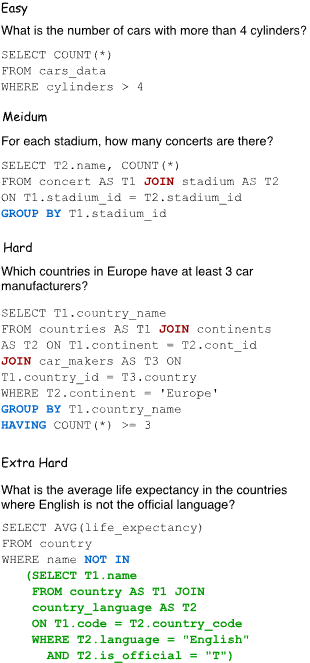
\includegraphics[width=0.35\textwidth]{image.png}
\caption{SQL query examples in 4 hardness levels. Credit: Spider [1]}
\label{fig:hardness-levels}
\end{figure}

\subsection{Prompting and Input}
\label{sec:prompting}

Each model receives three pieces of information in a single zero-shot user turn: a system instruction explaining its role as a Text-to-SQL generator, the database schema (table names, column names, primary keys, and foreign-key relationships, with no example rows), and the natural-language question. No few-shot examples are provided, so that the experiment measures each model's ability to generate SQL from instructions and schema information alone, without the confound of examples steering its output style. The prompt template is identical across all three models, so that differences in performance can be attributed to the models rather than to differences in prompting.

\textbf{Prompt template:}
\begin{verbatim}
Given the following SQLite database schema, write a SQL query that answers
the question.

{schema}

Question: {question}

Respond with only the SQL query in a ```sql code block.
\end{verbatim}

See \hyperref[sec:appendix1]{Appendix 1} for a worked example: a full schema, a question, and the resulting filled prompt.

\subsection{SQL Extraction}
\label{sec:sql-extraction}

For each sample, we decode the model's generated tokens into text using the model-specific tokenizer, and check for the presence of a \texttt{</think>} token. If \texttt{</think>} was generated, we take all text generated before \texttt{</think>} as the reasoning trace and all text to the right as the output SQL; DeepSeek-R1-Distill-Qwen-1.5B is the only model of the three that can emit this token. The SQL is then extracted from the first \texttt{```sql} code block in that remaining text. The extracted SQL is passed to the evaluation script as-is. Outputs that cannot be extracted or parsed are counted as incorrect on every metric rather than excluded from the evaluation, as unusable output is a task failure (see \ref{sec:evaluation-metrics} and \ref{sec:invalid-outputs}).

\subsection{Inference Settings}
\label{sec:inference-settings}

All models are evaluated using the same decoding configuration: greedy decoding (temperature and top-p are not applicable) for consistent, reproducible results between runs. The maximum output length differs by model: 256 tokens for Qwen3-0.6B, and 4096 tokens for both Qwen3-4B and DeepSeek-R1-Distill-Qwen-1.5B. For DeepSeek, the larger budget is needed because its output also has to contain a full reasoning trace rather than only the SQL query; Qwen3-4B is given the same, larger budget as DeepSeek so that a tighter token limit can be ruled out as the reason for any difference between them on invalid-output rate (\ref{sec:invalid-outputs}) or inference time (\ref{sec:efficiency}). Qwen3-0.6B and Qwen3-4B are both run with thinking mode off (both support it). DeepSeek-R1-Distill-Qwen-1.5B always produces a reasoning trace and has no documented way to disable thinking mode, so it is evaluated as the reasoning condition against the two non-reasoning Qwen3 models. All inference runs on the same 1x RTX 4090 GPU described in \ref{sec:models}, with batch size 1.

\subsection{Evaluation}
\label{sec:evaluation-metrics}

We evaluate the output using the same metrics as the Spider paper [1]. These are:

\begin{enumerate}
\item Component Matching
    \begin{itemize}
        \item For each of the following components:
        \begin{itemize}
            \item SELECT
            \item WHERE
            \item GROUP BY
            \item ORDER BY
            \item KEYWORDS (including all SQL keywords without column names and operators)
        \end{itemize}
        \item Decompose each component in the prediction and ground truth as bags of several sub-components and check whether or not these two sets of components match completely.
        \item Checks accuracy, recall, and F1
    \end{itemize}
\item Exact Matching Accuracy
    \begin{itemize}
        \item We measure whether the generated query as a whole is equivalent to the last section
        \item The generated query is correct only if all components are correct
        \item Checks only accuracy
    \end{itemize}
\item Execution Accuracy
    \begin{itemize}
        \item A list of gold values for each question is given
        \item We measure how many gold values the generated query extracts when executed
        \item Checks only accuracy
    \end{itemize}
\end{enumerate}

If output is invalid or unparsable, then it fails all 3 dimensions (component matching, exact matching, execution accuracy), consistent with how \ref{sec:sql-extraction} extracts and passes SQL to this evaluation script. This is reasonable as invalid/unparsable output cannot be applied to SQL and thus must be avoided and penalized heavily; Results~\ref{sec:invalid-outputs} reports how often this happens for each model.

\section{Task 1 -- RQ1: Results}
\label{sec:rq1-results}

\subsection{Overall Model Performance}
\label{sec:overall-performance}

Below we report how Qwen3-0.6B, Qwen3-4B, and Deepseek-R1-Distill-Qwen3-1.5B perform on the Spider benchmark across all 3 metrics (Component Matching, Exact Matching Accuracy, Execution Accuracy). We calculate the values per problem difficulty as well as overall, and display them in the below tables.

\begin{table}[H]
\centering
\footnotesize
\caption{Overall performance summary, aggregated across all difficulties (all 1034 problems). Component matching is accuracy / recall / F1 (macro-averaged, see the note on table~\ref{tab:difficulty-component} in \ref{sec:rq1-interpretation}). Per-difficulty breakdowns are in tables~\ref{tab:difficulty-component}--\ref{tab:difficulty-execution}.}
\label{tab:overall-performance}
\resizebox{\textwidth}{!}{%
\begin{tabular}{lllccc}
\toprule
Model & Parameters & Category & Component matching & Exact matching & Execution accuracy \\
\midrule
Qwen3-0.6B & 0.6B & Decoder-only & 0.628 / 0.209 / 0.314 & 0.099 & 0.209 \\
Qwen3-4B & 4B & Decoder-only & 0.797 / 0.306 / 0.442 & 0.256 & 0.353 \\
DeepSeek-R1-Distill-Qwen-1.5B & 1.5B & Reasoning & 0.661 / 0.174 / 0.275 & 0.085 & 0.121 \\
\bottomrule
\end{tabular}}
\end{table}

All models are evaluated zero-shot with the same prompt on the 20 databases of the Spider dev set. Aggregated across all difficulties and databases, every model is still far from solving the task: execution accuracy ranges from 0.121 (DeepSeek) to 0.353 (Qwen3-4B) and exact matching accuracy from 0.085 (DeepSeek) to 0.256 (Qwen3-4B). Execution accuracy is higher than exact matching accuracy for all three models (for example 0.353 vs.\ 0.256 for Qwen3-4B), which suggests that at least some of the queries that return the correct result are written differently from the gold SQL (see \ref{sec:rq1-interpretation} for more on this relationship). Of the three models, Qwen3-4B is now the best on almost every metric, database, and difficulty level; \ref{sec:by-database} and \ref{sec:rq1-interpretation} quantify how consistently. Table~\ref{tab:inference-time} reports the efficiency side of this comparison: inference time per example.

\subsection{Performance by Query Difficulty}
\label{sec:by-difficulty}

\begin{table}[H]
\centering
\footnotesize
\caption{Component matching (accuracy / recall / F1) by difficulty.}
\label{tab:difficulty-component}
\begin{tabular}{lcc}
\toprule
Model & easy & medium \\
\midrule
Problems (n) & 248 & 446 \\
Qwen3-0.6B & 0.675 / 0.308 / 0.423 & 0.582 / 0.235 / 0.334 \\
Qwen3-4B & 0.838 / 0.574 / 0.681 & 0.670 / 0.306 / 0.420 \\
DeepSeek-R1-Distill-Qwen-1.5B & 0.566 / 0.288 / 0.382 & 0.642 / 0.185 / 0.287 \\
\bottomrule
\end{tabular}

\vspace{0.5em}

\begin{tabular}{lccc}
\toprule
Model & hard & extra & all \\
\midrule
Problems (n) & 174 & 166 & 1034 \\
Qwen3-0.6B & 0.540 / 0.141 / 0.223 & 0.578 / 0.160 / 0.250 & 0.628 / 0.209 / 0.314 \\
Qwen3-4B & 0.796 / 0.262 / 0.394 & 0.485 / 0.150 / 0.229 & 0.797 / 0.306 / 0.442 \\
DeepSeek-R1-Distill-Qwen-1.5B & 0.543 / 0.113 / 0.187 & 0.389 / 0.104 / 0.164 & 0.661 / 0.174 / 0.275 \\
\bottomrule
\end{tabular}
\end{table}

\begin{table}[H]
\centering
\footnotesize
\caption{Exact matching accuracy by difficulty.}
\label{tab:difficulty-exact}
\begin{tabular}{lccccc}
\toprule
Model & easy & medium & hard & extra & all \\
\midrule
Problems (n) & 248 & 446 & 174 & 166 & 1034 \\
Qwen3-0.6B & 0.157 & 0.137 & 0.006 & 0.006 & 0.099 \\
Qwen3-4B & 0.508 & 0.262 & 0.115 & 0.012 & 0.256 \\
DeepSeek-R1-Distill-Qwen-1.5B & 0.214 & 0.078 & 0.000 & 0.000 & 0.085 \\
\bottomrule
\end{tabular}
\end{table}

\begin{table}[H]
\centering
\footnotesize
\caption{Execution accuracy by difficulty.}
\label{tab:difficulty-execution}
\begin{tabular}{lccccc}
\toprule
Model & easy & medium & hard & extra & all \\
\midrule
Problems (n) & 248 & 446 & 174 & 166 & 1034 \\
Qwen3-0.6B & 0.210 & 0.276 & 0.126 & 0.114 & 0.209 \\
Qwen3-4B & 0.565 & 0.345 & 0.276 & 0.139 & 0.353 \\
DeepSeek-R1-Distill-Qwen-1.5B & 0.258 & 0.128 & 0.017 & 0.006 & 0.121 \\
\bottomrule
\end{tabular}
\end{table}

We break every metric down by the Spider Hardness Criteria (\ref{sec:eval-data}) as query difficulty is a first-order driver of Text-to-SQL performance; comparing models only in aggregate would hide whether a model's advantage holds up as queries get harder.

Performance decreases with difficulty for every model, but the decrease is steepest for Qwen3-0.6B and DeepSeek: their exact matching and execution accuracy are both at most 0.034 and 0.126 respectively on hard and extra problems, down from as high as 0.210-0.258 (easy execution) on the easiest problems (table~\ref{tab:difficulty-exact} and table~\ref{tab:difficulty-execution}). Qwen3-4B degrades on the same relative scale but from a much higher starting point, from 0.508 easy exact matching / 0.565 easy execution accuracy down to 0.012 extra exact matching / 0.139 extra execution accuracy. Despite the degredation, it remains the best of the three models at every single difficulty level on both metrics (tables~\ref{tab:difficulty-exact}--\ref{tab:difficulty-execution}).

\subsection{Performance by Database}
\label{sec:by-database}

We also break execution and exact matching accuracy down by each of the 20 Spider dev databases. Qwen3-4B has the highest execution accuracy on 17 of the 20 databases outright (plus a tie on one more) and the highest exact matching accuracy on 18 of 20, while DeepSeek-R1-Distill-Qwen-1.5B is never highest on either metric; Qwen3-0.6B wins outright only on orchestra and battle\_death. Databases with few problems (real\_estate\_properties with n=4, voter\_1 with n=15, battle\_death with n=16, and museum\_visit with n=18) are too small to rank the models reliably, since a single problem changes a score by 6 to 25 percentage points. Execution accuracy ranges from 0.10 (course\_teach) to 0.53 (singer) for Qwen3-0.6B, from 0.19 (battle\_death) to 0.60 (singer) for Qwen3-4B, and from 0.00 (concert\_singer) to 0.27 (singer and voter\_1) for DeepSeek-R1-Distill-Qwen-1.5B (\hyperref[tab:db-execution]{Table 5}). The pattern on exact matching accuracy is just as one-sided (\hyperref[tab:db-exact]{Table 6}): Qwen3-4B is highest on 18 of 20 databases, ties Qwen3-0.6B on orchestra, and loses only on battle\_death; DeepSeek's exact matching accuracy is never the highest of the three, coming closest on flight\_2 (0.200 vs.\ Qwen3-4B's 0.350 and Qwen3-0.6B's 0.075). The full per-database tables and discussion are in \hyperref[sec:appendix2]{Appendix 2}.

\subsection{Invalid and Unparseable Outputs}
\label{sec:invalid-outputs}

We also count how often each model's output cannot be used as SQL at all: it either never produces a usable query within the token budget (\ref{sec:inference-settings}) or is truncated before finishing one. Per \ref{sec:evaluation-metrics}, these count as failures on every metric rather than being excluded, and this is a direct measure of how reliably each model follows the ``respond with only a SQL query'' instruction, independent of whether the SQL it does produce is correct. Qwen3-0.6B's invalid rate is 2.2\%, Qwen3-4B's is 0.0\%, and DeepSeek-R1-Distill-Qwen-1.5B's is 9.7\%, about 4x higher than Qwen3-0.6B's despite having the same 4096-token budget as Qwen3-4B (\ref{sec:inference-settings}), i.e. a larger token budget did not cause Qwen3-4B to run on or produce unusable output the way it does for DeepSeek. \ref{sec:rq1-interpretation} breaks DeepSeek's failures down further by difficulty and by why the generation failed (tables~\ref{tab:deepseek-outcome}--\ref{tab:deepseek-unfinished-by-difficulty}).

\subsection{Efficiency Measures}
\label{sec:efficiency}

\begin{table}[H]
\centering
\footnotesize
\caption{Output tokens per example}
\label{tab:tokens-per-example}
\begin{tabular}{lccccc}
\toprule
Model & easy & medium & hard & extra & all \\
\midrule
Qwen3-0.6B & 27.5 & 44.7 & 53.7 & 69.9 & 46.1 \\
Qwen3-4B & 23.6 & 37.3 & 46.2 & 59.0 & 39.0 \\
DeepSeek-R1-Distill-Qwen-1.5B & 610.8 & 768.4 & 1096.0 & 1176.9 & 851.3 \\
\bottomrule
\end{tabular}
\end{table}

Inference time is measured from the start of generation to the complete batch output, per batch of 1 example, excluding tokenization, model loading, and warm-up.

\begin{table}[H]
\centering
\footnotesize
\caption{Inference time.}
\label{tab:inference-time}
\begin{tabular}{lcc}
\toprule
Model & Total wall time (s) & Avg.\ time per example (s) \\
\midrule
Qwen3-0.6B & 123.9 & 0.120 \\
Qwen3-4B & 109.1 & 0.106 \\
DeepSeek-R1-Distill-Qwen-1.5B & 3059.8 & 2.959 \\
\bottomrule
\end{tabular}
\end{table}

DeepSeek is about 25x slower per example than Qwen3-0.6B and 28x slower than Qwen3-4B, consistent with its much higher average token count (table~\ref{tab:tokens-per-example}). Qwen3-4B, despite having about 7x as many parameters as Qwen3-0.6B, is marginally faster per example (0.106s vs.\ 0.120s), consistent with it generating fewer tokens on average (39.0 vs.\ 46.1, table~\ref{tab:tokens-per-example}) despite having the same 16x larger token budget as DeepSeek (\ref{sec:inference-settings}).

\begin{table}[H]
\centering
\footnotesize
\caption{DeepSeek-R1-Distill-Qwen-1.5B by generation outcome. ``Cut'' means the generation reached the 4096-token limit.}
\label{tab:deepseek-outcome}
\begin{tabular}{lccccc}
\toprule
Outcome & Problems (n) & Share & Avg.\ tokens & Exact match & Component F1 \\
\midrule
Finished with SQL & 934 & 90.3\% & 512 & 0.094 & 0.286 \\
Finished, no usable SQL & 2 & 0.2\% & 284 & 0.000 & 0.100 \\
Cut while answering (after \texttt{</think>}) & 13 & 1.3\% & 4096 & 0.000 & 0.096 \\
Cut while thinking (no \texttt{</think>}) & 85 & 8.2\% & 4096 & 0.000 & 0.093 \\
All & 1034 & 100\% & 851 & 0.085 & 0.275 \\
\bottomrule
\end{tabular}
\end{table}

\begin{table}[H]
\centering
\footnotesize
\caption{The same 934 questions that DeepSeek finished, for all three models.}
\label{tab:deepseek-finished-934}
\begin{tabular}{lcc}
\toprule
Model & Exact match & Component F1 \\
\midrule
DeepSeek-R1-Distill-Qwen-1.5B & 0.094 & 0.286 \\
Qwen3-0.6B & 0.103 & 0.317 \\
Qwen3-4B & 0.257 & 0.440 \\
\bottomrule
\end{tabular}
\end{table}

\begin{table}[H]
\centering
\footnotesize
\caption{Are the cut-off DeepSeek generations infinite self-repetition loops? A text that repeats itself compresses well, so a low compression ratio of the last 3000 characters indicates a loop.}
\label{tab:deepseek-repetition}
\begin{tabular}{lcccc}
\toprule
Generations & n & Median compression ratio & Ratio $<$ 0.15 & Last 150 characters repeat 3 or more times \\
\midrule
Cut off & 98 & 0.095 & 95.9\% & 96.9\% \\
Finished & 936 & 0.418 & 0.0\% & 0.2\% \\
\bottomrule
\end{tabular}
\end{table}

\begin{table}[H]
\centering
\footnotesize
\caption{Share of DeepSeek generations that did not finish with SQL, by difficulty.}
\label{tab:deepseek-unfinished-by-difficulty}
\begin{tabular}{lccccc}
\toprule
 & easy & medium & hard & extra & all \\
\midrule
Problems (n) & 248 & 446 & 174 & 166 & 1034 \\
Not finished with SQL (n) & 15 & 33 & 25 & 27 & 100 \\
Share & 6.0\% & 7.4\% & 14.4\% & 16.3\% & 9.7\% \\
\bottomrule
\end{tabular}
\end{table}

\section{Interpretation and Answer to Research Question (RQ1)}
\label{sec:rq1-interpretation}

\textbf{RQ1:} How do (selected) LLMs perform on cross-domain Text-to-SQL?

\vspace{10px}

All three models are still far from solving the task in this zero-shot setting: exact matching accuracy ranges from 0.085 to 0.256 and execution accuracy from 0.121 to 0.353 (table~\ref{tab:overall-performance}). Difficulty and database effects are discussed in \ref{sec:by-difficulty} and \ref{sec:by-database}; here we interpret the effects of model size and reasoning architecture and the exact-match/execution-accuracy relationship, and state the answer to RQ1 as three findings.

\textbf{First, within the Qwen family, scale is a strong and almost uniform predictor of performance, but an intermediate-size reasoning model from the Deepseek family still loses to the smallest model in the Qwen family.} Aggregated across all difficulties, Qwen3-4B has the best component matching (0.797 / 0.306 / 0.442), exact matching (0.256), and execution accuracy (0.353) of the three (table~\ref{tab:overall-performance}), and it beats Qwen3-0.6B on exact matching and execution accuracy at every individual difficulty level, including hard (0.115 vs.\ 0.006) and extra (0.012 vs.\ 0.006), where the smaller model solves almost nothing (tables~\ref{tab:difficulty-exact}--\ref{tab:difficulty-execution}). This is the largest, most consistent effect in the RQ1 results. The one exception is component matching on extra-hard problems, where Qwen3-0.6B's accuracy, recall, and F1 (0.578 / 0.160 / 0.250) are all slightly higher than Qwen3-4B's (0.485 / 0.150 / 0.229), the only point in the RQ1 results where the smaller Qwen3 model wins outright (table~\ref{tab:difficulty-component}). DeepSeek-R1-Distill-Qwen-1.5B sits between the two Qwen3 models in parameter count (1.5B) and is the only one that reasons, yet it is the lowest of the three on every aggregate metric (0.275 component F1, 0.085 exact matching, 0.121 execution accuracy) except its own component-matching accuracy (0.661 vs.\ 0.628 for Qwen3-0.6B). Thus, scale predicts performance well within a family, but does not transfer across the reasoning/non-reasoning boundary: having more parameters than Qwen3-0.6B did not help DeepSeek catch up to it.

\textbf{Second, the reasoning architecture itself, not parameter count, is the main driver of DeepSeek's low score.} Its invalid-output rate (9.7\%) is markedly higher than Qwen3-0.6B's (2.2\%) and Qwen3-4B's (0.0\% in this run) (\ref{sec:invalid-outputs}). In tables~\ref{tab:deepseek-outcome}--\ref{tab:deepseek-unfinished-by-difficulty}, 100 of 1034 generations (9.7\%) end without usable SQL. 85 never leave the reasoning phase, 13 are cut while writing the answer, and 2 finish without SQL. The number of unusable SQL generations also grows with difficulty, from 6.0\% on easy to 16.3\% on extra problems. These are not cases of long productive reasoning either: 95.9\% of the cut-off generations are highly self-repetitive (compression ratio below 0.15, median compression ratio 0.095, vs.\ 0.418 for finished generations), rewriting the same query and repeating phrases like ``So the final query is:'' without converging. Finishing does not make it better either: on the 934 questions DeepSeek does finish, its exact matching (0.094) and component F1 (0.286) are still below Qwen3-0.6B's on the same questions (0.103 / 0.317) and far below Qwen3-4B's (0.257 / 0.440), despite generating 512 tokens per question on average there, against 46 and 39 tokens overall for Qwen3-0.6B and Qwen3-4B (about 18x and 22x fewer). This extra length also costs time: DeepSeek is 25-28x slower per example than either Qwen3 model (\ref{sec:efficiency}). The reasoning trace mostly lengthens the output and sometimes never terminates, without improving the SQL when it does, and size alone is not the explanation, since Qwen3-4B is both bigger than DeepSeek and the best model in the comparison. Thus, reasoning architecture itself, not the parameter count, is the main driver of DeepSeek's low score.

\textbf{Third, query difficulty has a substantial, consistent effect on every model, including the best one.} Exact matching and execution accuracy both fall sharply from easy to extra-hard problems for all three models (\ref{sec:by-difficulty}). Qwen3-4B's drop is from a much higher base (0.508 to 0.012 exact matching, 0.565 to 0.139 execution accuracy) and it remains the best model at every difficulty level on both metrics, but the drop itself is just as steep in relative terms as for the other two models, and the hardest problems remain largely unsolved even for it.

\textbf{Exact match vs.\ execution accuracy.} For all three models, execution accuracy aggregated across all difficulties exceeds exact matching accuracy (table~\ref{tab:overall-performance}): 0.209 vs.\ 0.099 for Qwen3-0.6B, 0.353 vs.\ 0.256 for Qwen3-4B, and 0.121 vs.\ 0.085 for DeepSeek. Since exact matching requires every SQL component to match the gold query while execution accuracy only requires the same result set, this gap indicates each model writes some queries that are valid and correct but phrased differently from the gold SQL (e.g.\ a different but equivalent join order, or an explicit column list where the gold query uses \texttt{SELECT *}). The gap is widest for Qwen3-0.6B (11.0 points), close behind for Qwen3-4B (9.7 points), and narrowest for DeepSeek (3.6 points); DeepSeek's narrower gap reflects it producing fewer alternative-but-valid queries. Qwen3-4B's gap is almost as wide as Qwen3-0.6B's despite much higher absolute accuracy, so scaling up within the Qwen3 family raises both Exact Match Accuracy and Execution Accuracy together rather than closing the gap between them.

\textbf{Limitations.} Our working hypothesis is that Text-to-SQL at this scale does not benefit from an explicit reasoning trace, and that a non-reasoning model is sufficient, with performance instead scaling with parameter count within a fixed model family. The results are consistent with this hypothesis. However, they do not establish that Text-to-SQL is too simple for reasoning models in general due to several factors:

\begin{itemize}
\item \textbf{Truncation and failed outputs for DeepSeek.} These count as failures on every metric and lower its recall, exact matching, and execution scores, but table~\ref{tab:deepseek-finished-934} shows removing them would not change the ranking (DeepSeek is also lower on the questions it finished), and table~\ref{tab:deepseek-repetition} shows the cut-off generations are repetition loops, so a larger token budget is unlikely to rescue them.
\item \textbf{Model differences beyond reasoning.} Qwen3-0.6B and Qwen3-4B share a model family, isolating the effect of scale between them, but DeepSeek differs from both in family, size, and pretraining/post-training, not only in whether it reasons; it is also a distilled model, so the effect of reasoning cannot be fully separated from distillation quality.
\item \textbf{Aggregated component matching.} The component matching figures in table~\ref{tab:difficulty-component} (and in table~\ref{tab:overall-performance}) are our own macro-average (mean of the 10 per-component accuracy and recall scores, with F1 computed from these two means), not a number reported by Spider.
\end{itemize}

Overall, in this zero-shot, cross-domain setting, a larger non-reasoning decoder-only model (Qwen3-4B, 4B) clearly outperforms both a same-family model at under a sixth its size (Qwen3-0.6B) and a reasoning model of intermediate size from a different family (DeepSeek-R1-Distill-Qwen-1.5B, 1.5B), while also being faster per example than either. None of the three models solve more than half of even the easiest problems or more than a small fraction of hard or extra-hard queries. This answers RQ1 for the three models evaluated.
 (this
% file's cross-references into Task 1 -- table~\ref{tab:deepseek-outcome},
% \ref{tab:tokens-per-example}, \ref{sec:sql-extraction}, etc. -- rely on
% RQ1.tex's labels already being defined earlier in the same document).
%
% Structure: Methodology is organized per-feature (Feature 1: Token Count,
% Feature 2: Information Retention), each with its own Definition / Why it's
% relevant / How we computed it. Results is organized as descriptive
% statistics, differences by correctness, differences by difficulty, and
% relationship with Text-to-SQL correctness (the correlation analysis).

\section{Task 2 -- RQ2: Methodology}
\label{sec:rq2-methodology}

\textbf{RQ2:} How do characteristics of reasoning traces (of reasoning LLM) relate to Text-to-SQL performance?

To answer this question, we examine two features of each reasoning trace: Token Count and Information Retention. We compute both for all 1034 generations in DeepSeek-R1-Distill-Qwen-1.5B's main Task 1 run, then relate each to difficulty and to Text-to-SQL correctness.

\subsection{Feature 1: Token Count}
\label{sec:rq2-feature-tokencount}

\textbf{Definition.} Token Count is the number of tokens in the reasoning segment of a generation, i.e.\ everything the model generates before \texttt{</think>}, excluding the final SQL answer. We split each generation into a reasoning segment and an answer segment using the same \texttt{</think>} split used in Task 1 (\ref{sec:sql-extraction}).

\textbf{Why it's relevant.} We expect Token Count to scale positively with the difficulty of the related Text-to-SQL problem: easy questions should require fewer thinking tokens, while extra-hard questions should require significantly more. Any question that disobeys this relation, or where more tokens associate with worse rather than better answers, is given special attention in Results. Token Count is also the most direct, model-agnostic proxy we have for how much deliberation went into an answer, so it is a natural first feature to test against correctness.

\textbf{How we computed it.} Token Count is the number of tokens in the reasoning segment only, re-tokenized with the model's own tokenizer (not the \texttt{new\_tokens} field logged during generation, which counts the whole generation, reasoning plus SQL). For generations that never emit \texttt{</think>} (truncated at the 4096-token generation limit, see Task 1's table~\ref{tab:deepseek-outcome}), the entire generated text is treated as the reasoning segment, so Token Count for these rows is effectively capped at the generation limit rather than reflecting a completed thought. This is intentional: these cases are exactly the repetition loops Task 1 identified (table~\ref{tab:deepseek-repetition}), and dropping them would hide, rather than explain, the heavy right tail in Token Count. We keep them in the Token Count analysis and flag wherever they drive a result (see finding~\ref{item:rq2-finding-tokencount-difficulty} in Results).

\begin{table}[H]
\centering
\footnotesize
\caption{Token Count: definition and computation summary.}
\label{tab:rq2-feature-tokencount-summary}
\begin{tabular}{p{0.22\textwidth}p{0.7\textwidth}}
\toprule
Property & Detail \\
\midrule
Unit & Tokens (model's own tokenizer) \\
Scope & Reasoning segment only, i.e.\ text before \texttt{</think>} \\
Range & Non-negative integer, long right tail (observed 103--4166) \\
Truncated traces & Treated as reasoning segment in full; capped at the 4096-token generation limit \\
Hypothesis & Increases with difficulty; should not correlate with worse correctness \\
Test & Spearman's rank correlation vs.\ difficulty and vs.\ 32 per-question performance submetrics \\
\bottomrule
\end{tabular}
\end{table}

\subsection{Feature 2: Information Retention}
\label{sec:rq2-feature-retention}

\textbf{Definition.} Information Retention is the share of schema-shaped identifiers mentioned in a reasoning trace that actually exist as a table or column name in that question's schema. Equivalently, $1 - $ Information Retention is the hallucination rate of the trace: the fraction of mentioned identifiers that are not grounded in the prompt.

\textbf{Why it's relevant.} We expect reasoning traces with low Information Retention (frequent hallucination of schema elements) to produce lower-performing answers than traces that stay grounded in the given schema, since inventing a table or column that doesn't exist is very likely to propagate into an incorrect query. We also expect harder problems to not cause lower Information Retention on their own; if they do, this points to the model introducing more assumptions as questions get harder, which is itself worth investigating as a bias rather than attributing the accuracy drop to difficulty alone.

\textbf{How we computed it.} We regex-extract every schema-shaped identifier the trace mentions, either quoted (e.g.\ \texttt{"Singer\_ID"}) or underscore-joined (e.g.\ \texttt{concert\_id}), and take the share of those identifiers that match a table or column name in that question's schema. An identifier that matches neither is treated as a fact the model introduced on its own, i.e., a hallucination. Traces that mention no schema identifiers at all are excluded from Information Retention (but kept for Token Count), since a 0-of-0 ratio is undefined rather than evidence of perfect or zero retention; this drops the usable sample from 1034 to 1017. Truncated traces are scored the same way, over whatever partial text was generated.

\begin{table}[H]
\centering
\footnotesize
\caption{Information Retention: definition and computation summary.}
\label{tab:rq2-feature-retention-summary}
\begin{tabular}{p{0.22\textwidth}p{0.7\textwidth}}
\toprule
Property & Detail \\
\midrule
Unit & Ratio, bounded in $[0,1]$ \\
Numerator & Schema identifiers mentioned in the trace that match a real table/column name \\
Denominator & All schema-shaped identifiers mentioned in the trace (quoted or underscore-joined) \\
Exclusions & Traces mentioning zero schema identifiers (1034 $\rightarrow$ 1017 usable rows) \\
Truncated traces & Scored over the partial text generated before truncation \\
Hypothesis & Higher retention associates with better correctness; should not fall with difficulty \\
Test & Spearman's rank correlation vs.\ difficulty and vs.\ 32 per-question performance submetrics \\
\bottomrule
\end{tabular}
\end{table}

\subsection{Statistical approach}
\label{sec:rq2-statistical-approach}

We relate both Token Count and Information Retention to correctness and difficulty with Spearman's Rank Correlation throughout. Both of our hypotheses are about monotonic relationships, not linear relationships (performance should not decrease as Token Count or Information Retention increase, and Token Count should increase with difficulty), which is exactly what Spearman's Rank Correlation tests for. It also suits the distribution of our two reasoning metrics: Token Count is a non-negative count with a long right tail (DeepSeek alone ranges from 611 tokens on easy problems to 1177 on extra, table~\ref{tab:tokens-per-example}), and Information Retention is a bounded ratio, so neither is likely to be symmetric and unbounded; the $\geq$90\% trace completion rate gives us enough data per stratum to check this on histograms rather than assume it. For correctness, we correlate each reasoning metric against the continuous, per-question component matching accuracy, recall, and F1 for all ten Spider components individually, plus exact matching and execution accuracy, rather than collapsing them into one pass/fail label, which keeps the per-question variance in performance a binary cutoff would discard and sidesteps splitting by correctness directly, which is not viable per difficulty level: DeepSeek's exact matching accuracy falls to at most 0.034 on hard and extra problems, leaving as few as four to six correct traces in those strata. This gives 32 submetrics per reasoning metric per difficulty level. We chose this rank-based, continuous-correlation approach over a parametric correlation or a correct/incorrect group comparison because our data is too skewed for the former and our correct-answer strata too sparse for the latter. With 169 correlation tests run in total, we correct for multiple comparisons with the Benjamini-Hochberg procedure rather than a stricter family-wise correction like Bonferroni: we are screening many related, non-independent submetrics for the strongest associations to report and discuss, not making a small number of pre-registered confirmatory claims, so controlling the expected false-discovery rate is a better fit than controlling the probability of any single false positive at the cost of statistical power.

The Results below report Token Count and Information Retention broken down two ways: by difficulty, since that is the primary hypothesis under test, and by exact-match correctness (correct/incorrect), used for the descriptive statistics and the boxplots (figure~\ref{fig:rq2-boxplots}) because a binary split is easier to read in a table or figure than 32 continuous submetrics. The correlation analysis itself (table~\ref{tab:rq2-correlations}) still uses the continuous submetrics described above, for the statistical-power reasons given there; the binary-correctness view and the continuous-submetric view are two presentations of the same underlying data, not two different analyses.

\textbf{Verification.} To check that the Spearman findings above are not artifacts of one particular rank-based method or of an unmodeled confound, we add two further layers of testing, reported in \ref{sec:rq2-verification} and \ref{sec:rq2-robustness}. First, we run two confirmatory, feature-specific significance tests directly on the binary/ordinal views used for the descriptive statistics: a Mann-Whitney U test for each feature against exact-match correctness (overall and within each difficulty stratum), and Kendall's tau-b for each feature against difficulty (overall and within each correctness stratum). We prefer Kendall's tau-b over a second Spearman run here because it is the standard choice when one variable has many ties (difficulty has only four distinct values, and Information Retention has a large tied mass at 1.0), and it is the ordered-groups analogue of the Jonckheere-Terpstra trend test. Second, because Token Count, Information Retention and difficulty are all correlated with one another, a bivariate relationship between one feature and an outcome could simply be riding on the other two variables rather than reflecting an independent association. We fit two regression models to check this: a logistic regression of exact-match correctness on standardized log Token Count, standardized Information Retention, and standardized difficulty, all entered jointly; and a proportional-odds (ordinal) regression of difficulty on standardized log Token Count and standardized Information Retention, entered jointly. Token Count is log-transformed before standardizing given its heavy right skew (see above); difficulty enters the logistic model as a single linear control on the log-odds scale, which is a simplification rather than a full categorical treatment, and the ordinal model assumes proportional odds across the three difficulty thresholds, which we did not separately test -- both are limitations of this robustness check, not of the primary Spearman analysis. All four verification tests and both regression models are implemented in \texttt{eval/evalpipeline/reasoning\_verification.py}, run on the same per-question table as the Spearman analysis.

\section{Task 2 -- RQ2: Results}
\label{sec:rq2-results}

We compute Token Count and Information Retention for all 1034 generations in DeepSeek-R1-Distill-Qwen-1.5B's main Task 1 run, and correlate each against difficulty and against all 32 per-question performance submetrics as described in the Methodology. Table~\ref{tab:rq2-descriptive-stats-tokencount} and table~\ref{tab:rq2-descriptive-stats-retention} give descriptive statistics for each feature by difficulty and by exact-match correctness; figure~\ref{fig:rq2-boxplots} shows the resulting distributions; table~\ref{tab:rq2-correlations} lists the strongest correlations.

\subsection{Descriptive statistics}
\label{sec:rq2-descriptive-stats}

\begin{table}[H]
\centering
\footnotesize
\caption{Token Count descriptive statistics, by difficulty and by exact-match correctness (1 = exact match, 0 = not). Full results in \texttt{eval/results/task2\_analysis/descriptive\_stats.csv}.}
\label{tab:rq2-descriptive-stats-tokencount}
\begin{tabular}{lcccccc}
\toprule
Group & n & mean & median & std & min & max \\
\midrule
easy & 248 & 542.3 & 329.0 & 845.2 & 103 & 4096 \\
medium & 446 & 648.2 & 374.0 & 925.7 & 191 & 4166 \\
hard & 174 & 939.2 & 425.0 & 1246.2 & 226 & 4096 \\
extra & 166 & 901.6 & 434.5 & 1199.9 & 222 & 4096 \\
\midrule
exact match = 0 & 946 & 748.1 & 394.0 & 1065.6 & 103 & 4166 \\
exact match = 1 & 88 & 329.3 & 314.5 & 97.7 & 195 & 849 \\
\midrule
all & 1034 & 712.4 & 383.0 & 1026.2 & 103 & 4166 \\
\bottomrule
\end{tabular}
\end{table}

\begin{table}[H]
\centering
\footnotesize
\caption{Information Retention descriptive statistics, by difficulty and by exact-match correctness (1 = exact match, 0 = not). Excludes traces that mention no schema identifiers (n drops from 1034 to 1017 overall). Full results in \texttt{eval/results/task2\_analysis/descriptive\_stats.csv}.}
\label{tab:rq2-descriptive-stats-retention}
\begin{tabular}{lcccccc}
\toprule
Group & n & mean & median & std & min & max \\
\midrule
easy & 246 & 0.915 & 1.0 & 0.146 & 0.0 & 1.0 \\
medium & 441 & 0.905 & 1.0 & 0.148 & 0.0 & 1.0 \\
hard & 172 & 0.877 & 1.0 & 0.163 & 0.0 & 1.0 \\
extra & 158 & 0.861 & 1.0 & 0.215 & 0.0 & 1.0 \\
\midrule
exact match = 0 & 931 & 0.893 & 1.0 & 0.166 & 0.0 & 1.0 \\
exact match = 1 & 86 & 0.924 & 1.0 & 0.123 & 0.5 & 1.0 \\
\midrule
all & 1017 & 0.896 & 1.0 & 0.163 & 0.0 & 1.0 \\
\bottomrule
\end{tabular}
\end{table}

\begin{figure}[H]
\centering
\includegraphics[width=0.95\textwidth]{boxplots.png}
\caption{Token Count and Information Retention by difficulty and by exact-match correctness, for DeepSeek-R1-Distill-Qwen-1.5B's 1034 Task 1 generations. Green triangles are means, orange lines are medians. Means sit well above medians throughout, confirming the right-skewed, bounded distributions the Methodology assumes rather than normal ones.}
\label{fig:rq2-boxplots}
\end{figure}

\subsection{Differences by correctness}
\label{sec:rq2-by-correctness}

Correct generations (exact match = 1) have a much lower mean and tighter spread of Token Count (329.3, std 97.7) than incorrect ones (748.1, std 1065.6, table~\ref{tab:rq2-descriptive-stats-tokencount}), and a slightly higher mean Information Retention (0.924 vs.\ 0.893, table~\ref{tab:rq2-descriptive-stats-retention}). Both differences point the same direction as the correlation findings in \ref{sec:rq2-relationship-correctness}: more reasoning tokens and lower retention associate with worse performance. The gap is far larger for Token Count than for Information Retention: incorrect generations' Token Count std (1065.6) is more than ten times that of correct generations (97.7), driven by the truncated, repetition-loop traces described in \ref{sec:rq2-feature-tokencount}, almost none of which are exact matches. Information Retention's median is 1.0 in both correctness groups, so the correctness gap in retention lives entirely in the mean and the lower tail, not in a shift of the typical trace.

\subsection{Differences by difficulty}
\label{sec:rq2-by-difficulty}

\begin{enumerate}
\item \label{item:rq2-finding-tokencount-difficulty} \textbf{Token Count increases with difficulty, as hypothesized, but the increase is driven by a heavy tail.} Median token count rises from 329 (easy) to 374 (medium) to 425 (hard) to 434 (extra), and the correlation with difficulty is positive and significant ($\rho=0.313$, $q<0.001$). The mean rises faster than the median at every level (for example 542 vs.\ 329 on easy), because generations hitting the 4096-token limit occur at every difficulty (figure~\ref{fig:rq2-boxplots}, top row); these are the same repetition loops Task 1 identified, not productive extra reasoning on harder problems.
\item \label{item:rq2-finding-retention-difficulty} \textbf{Information Retention decreases slightly with difficulty.} Median retention is 1.0 at every difficulty level, but the mean falls from 0.915 (easy) to 0.861 (extra), and the correlation with difficulty is negative and significant ($\rho=-0.107$, $q=0.013$). Per the Methodology, this is the case that calls for examining the model's introduced assumptions on harder problems rather than attributing the accuracy drop to difficulty alone.
\end{enumerate}

\subsection{Relationship with Text-to-SQL correctness}
\label{sec:rq2-relationship-correctness}

\begin{enumerate}
\item \label{item:rq2-finding-tokencount-disobey} \textbf{On easy and medium problems, more Token Count tracks worse performance, the ``disobeying'' case flagged in the Methodology.} Token Count correlates negatively with \texttt{keywords} F1 on easy ($\rho=-0.42$, $q<0.001$) and medium ($\rho=-0.19$, $q=0.001$) problems, and with \texttt{where} and \texttt{where(no OP)} F1 on easy problems ($\rho=-0.32$ and $-0.33$, $q<0.001$). Combined with finding~\ref{item:rq2-finding-tokencount-difficulty}, the extra tokens on these problems look like run-away generation rather than helpful deliberation.
\item \label{item:rq2-finding-retention-performance} \textbf{Where Information Retention does relate to performance, it is positive, as hypothesized.} On medium problems, Information Retention correlates positively with \texttt{where} and \texttt{where(no OP)} F1 ($\rho=0.345$, $q<0.001$ for both), consistent with higher-retention traces producing more accurate WHERE clauses. Of the 169 tests run, 26 remain significant after Benjamini-Hochberg correction; the strongest are in table~\ref{tab:rq2-correlations}.
\end{enumerate}

\begin{table}[H]
\centering
\footnotesize
\caption{Strongest Spearman correlations between reasoning metrics and performance submetrics, Benjamini-Hochberg corrected, top 8 of 169 tests by q-value. Full results in \texttt{eval/results/task2\_analysis/spearman\_correlations.csv}.}
\label{tab:rq2-correlations}
\begin{tabular}{llcccc}
\toprule
Metric & Submetric & Difficulty & n & $\rho$ & $q$ \\
\midrule
Token Count & difficulty (overall) & all & 1034 & 0.313 & $<$0.001 \\
Information Retention & where F1 & medium & 441 & 0.345 & $<$0.001 \\
Information Retention & where(no OP) F1 & medium & 441 & 0.345 & $<$0.001 \\
Token Count & keywords F1 & easy & 248 & -0.417 & $<$0.001 \\
Token Count & where(no OP) F1 & easy & 248 & -0.332 & $<$0.001 \\
Token Count & where F1 & easy & 248 & -0.322 & $<$0.001 \\
Token Count & keywords F1 & medium & 446 & -0.194 & $<$0.001 \\
Information Retention & difficulty (overall) & all & 1017 & -0.107 & 0.013 \\
\bottomrule
\end{tabular}
\end{table}

\subsection{Verification: Mann-Whitney U and Kendall's tau-b}
\label{sec:rq2-verification}

\begin{table}[H]
\centering
\footnotesize
\caption{Mann-Whitney U test: Token Count by exact-match correctness, overall and within each difficulty stratum. $r$ is the rank-biserial correlation (negative = higher Token Count associates with incorrect answers). Full results in \texttt{eval/results/task2\_analysis/mann\_whitney\_tokencount.csv}.}
\label{tab:rq2-mw-tokencount}
\begin{tabular}{lccccc}
\toprule
Stratum & n(incorrect) & n(correct) & $U$ & $p$ & $r$ \\
\midrule
all & 946 & 88 & 60406.5 & $<$0.001 & -0.451 \\
easy & 195 & 53 & 6423.0 & 0.007 & -0.243 \\
medium & 411 & 35 & 9644.0 & 0.001 & -0.341 \\
hard & 174 & 0 & --- & --- & --- \\
extra & 166 & 0 & --- & --- & --- \\
\bottomrule
\end{tabular}
\end{table}

\begin{table}[H]
\centering
\footnotesize
\caption{Mann-Whitney U test: Information Retention by exact-match correctness, overall and within each difficulty stratum. Full results in \texttt{eval/results/task2\_analysis/mann\_whitney\_retention.csv}.}
\label{tab:rq2-mw-retention}
\begin{tabular}{lccccc}
\toprule
Stratum & n(incorrect) & n(correct) & $U$ & $p$ & $r$ \\
\midrule
all & 931 & 86 & 36583.5 & 0.136 & 0.086 \\
easy & 194 & 52 & 5245.0 & 0.601 & -0.040 \\
medium & 407 & 34 & 5989.0 & 0.137 & 0.134 \\
hard & 172 & 0 & --- & --- & --- \\
extra & 158 & 0 & --- & --- & --- \\
\bottomrule
\end{tabular}
\end{table}

\begin{table}[H]
\centering
\footnotesize
\caption{Kendall's tau-b: Token Count vs.\ difficulty, overall and within each correctness stratum. Full results in \texttt{eval/results/task2\_analysis/kendall\_tokencount.csv}.}
\label{tab:rq2-kendall-tokencount}
\begin{tabular}{lccc}
\toprule
Group & n & $\tau_b$ & $p$ \\
\midrule
all & 1034 & 0.239 & $<$0.001 \\
incorrect & 946 & 0.207 & $<$0.001 \\
correct & 88 & 0.130 & 0.141 \\
\bottomrule
\end{tabular}
\end{table}

\begin{table}[H]
\centering
\footnotesize
\caption{Kendall's tau-b: Information Retention vs.\ difficulty, overall and within each correctness stratum. Full results in \texttt{eval/results/task2\_analysis/kendall\_retention.csv}.}
\label{tab:rq2-kendall-retention}
\begin{tabular}{lccc}
\toprule
Group & n & $\tau_b$ & $p$ \\
\midrule
all & 1017 & -0.091 & $<$0.001 \\
incorrect & 931 & -0.093 & $<$0.001 \\
correct & 86 & 0.110 & 0.279 \\
\bottomrule
\end{tabular}
\end{table}

Token Count's relationship with correctness is confirmed by the Mann-Whitney test: the overall gap is highly significant ($p<0.001$) with a moderate rank-biserial effect ($r=-0.451$), and it holds up within both the easy ($p=0.007$) and medium ($p=0.001$) strata individually. Hard and extra cannot be tested at all, because this run has zero exact matches in either stratum (table~\ref{tab:rq2-mw-tokencount}) -- a direct, concrete confirmation of the Methodology's reason for using continuous correlation instead of a correctness split per difficulty level. Information Retention's correctness gap, by contrast, is \emph{not} statistically significant overall ($p=0.136$, table~\ref{tab:rq2-mw-retention}): the descriptive mean difference noted in \ref{sec:rq2-by-correctness} (0.924 vs.\ 0.893) is not large enough relative to the within-group spread to rule out chance at this sample size.

Kendall's tau-b replicates the Spearman difficulty trend for both features using a method that does not rely on an equal-interval difficulty scale and is designed for heavily tied data: Token Count's $\tau_b=0.239$ ($p<0.001$) is consistent in sign and significance with its Spearman $\rho=0.313$, and Information Retention's $\tau_b=-0.091$ ($p<0.001$) is consistent with its Spearman $\rho=-0.107$ (tables~\ref{tab:rq2-kendall-tokencount}--\ref{tab:rq2-kendall-retention}). Both trends replicate within the much larger incorrect stratum (931--946 rows) but are not significant within the sparse correct stratum (86--88 rows, $p=0.141$ and $0.279$), which is expected given the large drop in sample size rather than evidence against the trend.

\subsection{Robustness: controlling for confounds}
\label{sec:rq2-robustness}

\begin{table}[H]
\centering
\footnotesize
\caption{Logistic regression: exact match on standardized log Token Count, standardized Information Retention, and standardized difficulty, fit jointly ($n=1017$, pseudo $R^2=0.188$). OR is the odds ratio per one-SD increase in the predictor. Full results in \texttt{eval/results/task2\_analysis/logistic\_regression.csv}.}
\label{tab:rq2-logistic}
\begin{tabular}{lccccc}
\toprule
Predictor & coef & SE & $z$ & $p$ & OR [95\% CI] \\
\midrule
Intercept & -3.351 & 0.227 & -14.76 & $<$0.001 & 0.035 [0.022, 0.055] \\
log Token Count ($z$) & -1.087 & 0.300 & -3.62 & $<$0.001 & 0.337 [0.187, 0.607] \\
Information Retention ($z$) & 0.091 & 0.139 & 0.65 & 0.514 & 1.095 [0.834, 1.437] \\
Difficulty ($z$) & -1.278 & 0.201 & -6.35 & $<$0.001 & 0.279 [0.188, 0.413] \\
\bottomrule
\end{tabular}
\end{table}

\begin{table}[H]
\centering
\footnotesize
\caption{Proportional-odds (ordinal) regression: difficulty on standardized log Token Count and standardized Information Retention, fit jointly ($n=1017$). OR is the odds ratio per one-SD increase in the predictor. Full results in \texttt{eval/results/task2\_analysis/ordinal\_regression.csv}.}
\label{tab:rq2-ordinal}
\begin{tabular}{lccccc}
\toprule
Predictor & coef & SE & $z$ & $p$ & OR [95\% CI] \\
\midrule
log Token Count ($z$) & 0.398 & 0.059 & 6.78 & $<$0.001 & 1.489 [1.327, 1.670] \\
Information Retention ($z$) & -0.177 & 0.059 & -2.99 & 0.003 & 0.837 [0.746, 0.941] \\
\bottomrule
\end{tabular}
\end{table}

Controlling for the other feature and for difficulty changes which bivariate relationship survives. Token Count's association with correctness holds up: each one-SD increase in log Token Count is associated with 66\% lower odds of an exact match (OR$=0.337$, $p<0.001$), holding Information Retention and difficulty fixed (table~\ref{tab:rq2-logistic}) -- consistent with, and strengthening, finding~\ref{item:rq2-finding-tokencount-disobey}. Information Retention's association with correctness does not survive the same control (OR$=1.095$, $p=0.514$): once Token Count and difficulty are accounted for, Retention has no detectable independent effect on correctness, so the positive finding in \ref{item:rq2-finding-retention-performance} should be read as a submetric-specific, not a global, relationship. Both features' difficulty relationships, in contrast, are independent of one another: the ordinal regression finds Token Count still predicts higher difficulty (OR$=1.489$ per SD, $p<0.001$) and Information Retention still predicts lower difficulty (OR$=0.837$ per SD, $p=0.003$) when controlling for each other (table~\ref{tab:rq2-ordinal}), so neither difficulty trend in \ref{sec:rq2-by-difficulty} is simply a byproduct of the other feature's trend.
 into REPORT.tex, after % RQ1.tex -- Task 1 / RQ1 section, factored out of REPORT.tex.
%
% Intended use: % RQ1.tex -- Task 1 / RQ1 section, factored out of REPORT.tex.
%
% Intended use: \input{RQ1.tex} into REPORT.tex in place of the current inline
% "Task 1 -- RQ1: Methodology & Results" / "Task 1 -- RQ1: Results" content.
% REPORT.tex already loads every package this fragment needs (booktabs, array,
% graphicx, float, caption, hyperref), so no extra preamble is required.
%
% Annotations made while converting this to reference-based numbering:
%  - All \subsection*{N.M ...} / \section*{...} became real, numbered
%    \section/\subsection commands with the leading "N.M" stripped from the
%    title text (LaTeX now generates it), each with a \label. The former
%    \subsection*{3. Interpretation...} is promoted to a top-level \section,
%    since it was already numbered as a peer of Parts 1 and 2, not a child
%    of Part 2.
%  - Every table/figure got a \label right after its \caption, and every
%    in-text "table 1", "tables 2-4", "2.2", "Appendix 2", etc. became a
%    \ref (or \hyperref for Appendix 2/3, which live outside this file --
%    see note below). Because the Models table (1.1) is now counted and the
%    Appendix 2/3 tables are not part of this file's sequential numbering,
%    the printed table numbers shift versus the pasted draft (e.g. "table 1"
%    -> Table 2, "table 8" -> Table 6); every mention uses \ref, so this is
%    self-consistent and will stay correct if tables move again.
%  - Fixed a leftover inconsistency in 1.5: the draft's 1.1 and 2.5 both
%    state batch size 1 (confirmed correct), but 1.5 still said "batch size
%    128" (leftover from an earlier draft) -- corrected to 1.
%  - Both TODOs in the pasted draft are resolved inline: 2.2 now cites
%    Tables 4-5 directly instead of a placeholder, and 2.3 now cites the
%    concrete per-database numbers from Appendix 2 (pulled from REPORT.tex's
%    existing Appendix 2 prose) instead of a placeholder.
%  - The Overall Performance table's caption promises "the note on table 2
%    in 3" (i.e. a note about macro-averaged component matching, to appear
%    in the Interpretation section), but the pasted draft's Limitations list
%    dropped that bullet (it only kept "Truncation" and "Model differences").
%    Restored the "Aggregated component matching" bullet from the prior
%    REPORT.tex draft so the caption's forward reference resolves to real
%    content; this is a content restoration, not just a labeling change,
%    so flagging it here. The other previously-present bullet ("Single run
%    and sample size") was NOT restored, since nothing in the new draft
%    points to it -- worth confirming with the author whether that drop was
%    intentional.
%  - Appendix 1/2/3 and their tables (5, 6, 7) live in REPORT.tex, outside
%    this file. REPORT.tex's appendix tables keep their existing manual
%    "Table 5/6/7:" caption numbering (renumbering them would require
%    restructuring the whole document's table order, which is out of scope
%    here); \label{tab:db-execution}, \label{tab:db-exact} and
%    \label{tab:invalid-outputs} were added to those tables in REPORT.tex
%    (additive only, no visible change) so this file can link to them.
%    Since their printed numbers are not auto-generated, this file links to
%    them with \hyperref[label]{5}-style calls (a real clickable link, with
%    text matching the manual number already in their caption) rather than
%    \ref (which would print whatever their true document-order table
%    number is, not 5/6/7).

\section{Task 1 -- RQ1: Methodology \& Results}
\label{sec:rq1-methods}

\textbf{RQ1:} How do (selected) LLMs perform on cross-domain Text-to-SQL?

In this report we evaluate the performance of decoder-only language models as well as reasoning LLMs on cross-domain SQL.

\subsection{Models}
\label{sec:models}

We compare two decoder-only LLMs from the same model family at different scales (Qwen3-0.6B and Qwen3-4B) against one reasoning LLM, so that the comparison isolates the effect of scale within a fixed family from the effect of an explicit reasoning trace, as much as a 3-model study can. All three are accessed as local inference over their bf16 Huggingface checkpoints on 1x NVIDIA GeForce RTX 4090 GPU (no API-based models), so that inference parameters are fully under our control (see \ref{sec:inference-settings}). We evaluate using batch sizes of 1.

\begin{table}[H]
\centering
\footnotesize
\caption{Models compared in RQ1.}
\label{tab:models}
\resizebox{\textwidth}{!}{%
\begin{tabular}{llllll}
\toprule
Model & Category & Parameters & Quantization & Access & Thinking mode \\
\midrule
Qwen3-0.6B [2] & Decoder-only & 0.6B & bf16 (none beyond release precision) & Local, Huggingface checkpoint & Disabled \\
Qwen3-4B [2] & Decoder-only & 4B & bf16 (none beyond release precision) & Local, Huggingface checkpoint & Disabled \\
DeepSeek-R1-Distill-Qwen-1.5B [4] & Reasoning & 1.5B & bf16 (none beyond release precision) & Local, Huggingface checkpoint & Always on (no disable option) \\
\bottomrule
\end{tabular}}
\end{table}

All three are dense (non-MoE) models, so no distinction between total and active parameters applies.

\subsection{Evaluation Data}
\label{sec:eval-data}

We use all 1034 examples in the Spider [1] development split, with no subsampling and therefore no sampling seed to report; every example is included, so the per-database counts below and the per-database results tables (\hyperref[tab:db-execution]{5} and \hyperref[tab:db-exact]{6}) enumerate exactly which examples are used. To evaluate cross-domain performance, we additionally report results separately for each of the 20 databases in the Spider dev set: world\_1 (120 problems), car\_1 (92), cre\_Doc\_Template\_Mgt (84), dog\_kennels (82), flight\_2 (80), student\_transcripts\_tracking (78), wta\_1 (62), tvshow (62), network\_1 (56), concert\_singer (45), pets\_1 (42), poker\_player (40), orchestra (40), employee\_hire\_evaluation (38), course\_teach (30), singer (30), museum\_visit (18), battle\_death (16), voter\_1 (15), and real\_estate\_properties (4).

We also use the Spider Hardness Criteria, where queries are assigned difficulties based on the number of SQL components, selections, and conditions, so that queries that contain more SQL keywords are considered harder.

\begin{figure}[H]
\centering
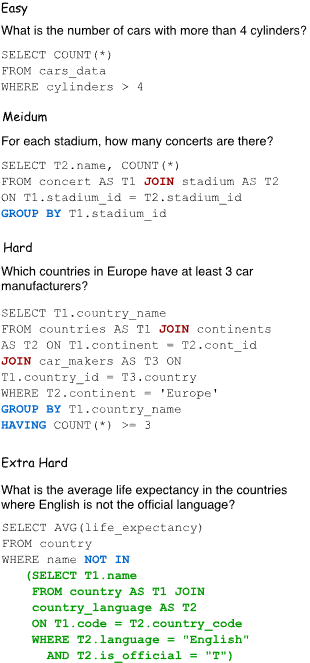
\includegraphics[width=0.35\textwidth]{image.png}
\caption{SQL query examples in 4 hardness levels. Credit: Spider [1]}
\label{fig:hardness-levels}
\end{figure}

\subsection{Prompting and Input}
\label{sec:prompting}

Each model receives three pieces of information in a single zero-shot user turn: a system instruction explaining its role as a Text-to-SQL generator, the database schema (table names, column names, primary keys, and foreign-key relationships, with no example rows), and the natural-language question. No few-shot examples are provided, so that the experiment measures each model's ability to generate SQL from instructions and schema information alone, without the confound of examples steering its output style. The prompt template is identical across all three models, so that differences in performance can be attributed to the models rather than to differences in prompting.

\textbf{Prompt template:}
\begin{verbatim}
Given the following SQLite database schema, write a SQL query that answers
the question.

{schema}

Question: {question}

Respond with only the SQL query in a ```sql code block.
\end{verbatim}

See \hyperref[sec:appendix1]{Appendix 1} for a worked example: a full schema, a question, and the resulting filled prompt.

\subsection{SQL Extraction}
\label{sec:sql-extraction}

For each sample, we decode the model's generated tokens into text using the model-specific tokenizer, and check for the presence of a \texttt{</think>} token. If \texttt{</think>} was generated, we take all text generated before \texttt{</think>} as the reasoning trace and all text to the right as the output SQL; DeepSeek-R1-Distill-Qwen-1.5B is the only model of the three that can emit this token. The SQL is then extracted from the first \texttt{```sql} code block in that remaining text. The extracted SQL is passed to the evaluation script as-is. Outputs that cannot be extracted or parsed are counted as incorrect on every metric rather than excluded from the evaluation, as unusable output is a task failure (see \ref{sec:evaluation-metrics} and \ref{sec:invalid-outputs}).

\subsection{Inference Settings}
\label{sec:inference-settings}

All models are evaluated using the same decoding configuration: greedy decoding (temperature and top-p are not applicable) for consistent, reproducible results between runs. The maximum output length differs by model: 256 tokens for Qwen3-0.6B, and 4096 tokens for both Qwen3-4B and DeepSeek-R1-Distill-Qwen-1.5B. For DeepSeek, the larger budget is needed because its output also has to contain a full reasoning trace rather than only the SQL query; Qwen3-4B is given the same, larger budget as DeepSeek so that a tighter token limit can be ruled out as the reason for any difference between them on invalid-output rate (\ref{sec:invalid-outputs}) or inference time (\ref{sec:efficiency}). Qwen3-0.6B and Qwen3-4B are both run with thinking mode off (both support it). DeepSeek-R1-Distill-Qwen-1.5B always produces a reasoning trace and has no documented way to disable thinking mode, so it is evaluated as the reasoning condition against the two non-reasoning Qwen3 models. All inference runs on the same 1x RTX 4090 GPU described in \ref{sec:models}, with batch size 1.

\subsection{Evaluation}
\label{sec:evaluation-metrics}

We evaluate the output using the same metrics as the Spider paper [1]. These are:

\begin{enumerate}
\item Component Matching
    \begin{itemize}
        \item For each of the following components:
        \begin{itemize}
            \item SELECT
            \item WHERE
            \item GROUP BY
            \item ORDER BY
            \item KEYWORDS (including all SQL keywords without column names and operators)
        \end{itemize}
        \item Decompose each component in the prediction and ground truth as bags of several sub-components and check whether or not these two sets of components match completely.
        \item Checks accuracy, recall, and F1
    \end{itemize}
\item Exact Matching Accuracy
    \begin{itemize}
        \item We measure whether the generated query as a whole is equivalent to the last section
        \item The generated query is correct only if all components are correct
        \item Checks only accuracy
    \end{itemize}
\item Execution Accuracy
    \begin{itemize}
        \item A list of gold values for each question is given
        \item We measure how many gold values the generated query extracts when executed
        \item Checks only accuracy
    \end{itemize}
\end{enumerate}

If output is invalid or unparsable, then it fails all 3 dimensions (component matching, exact matching, execution accuracy), consistent with how \ref{sec:sql-extraction} extracts and passes SQL to this evaluation script. This is reasonable as invalid/unparsable output cannot be applied to SQL and thus must be avoided and penalized heavily; Results~\ref{sec:invalid-outputs} reports how often this happens for each model.

\section{Task 1 -- RQ1: Results}
\label{sec:rq1-results}

\subsection{Overall Model Performance}
\label{sec:overall-performance}

Below we report how Qwen3-0.6B, Qwen3-4B, and Deepseek-R1-Distill-Qwen3-1.5B perform on the Spider benchmark across all 3 metrics (Component Matching, Exact Matching Accuracy, Execution Accuracy). We calculate the values per problem difficulty as well as overall, and display them in the below tables.

\begin{table}[H]
\centering
\footnotesize
\caption{Overall performance summary, aggregated across all difficulties (all 1034 problems). Component matching is accuracy / recall / F1 (macro-averaged, see the note on table~\ref{tab:difficulty-component} in \ref{sec:rq1-interpretation}). Per-difficulty breakdowns are in tables~\ref{tab:difficulty-component}--\ref{tab:difficulty-execution}.}
\label{tab:overall-performance}
\resizebox{\textwidth}{!}{%
\begin{tabular}{lllccc}
\toprule
Model & Parameters & Category & Component matching & Exact matching & Execution accuracy \\
\midrule
Qwen3-0.6B & 0.6B & Decoder-only & 0.628 / 0.209 / 0.314 & 0.099 & 0.209 \\
Qwen3-4B & 4B & Decoder-only & 0.797 / 0.306 / 0.442 & 0.256 & 0.353 \\
DeepSeek-R1-Distill-Qwen-1.5B & 1.5B & Reasoning & 0.661 / 0.174 / 0.275 & 0.085 & 0.121 \\
\bottomrule
\end{tabular}}
\end{table}

All models are evaluated zero-shot with the same prompt on the 20 databases of the Spider dev set. Aggregated across all difficulties and databases, every model is still far from solving the task: execution accuracy ranges from 0.121 (DeepSeek) to 0.353 (Qwen3-4B) and exact matching accuracy from 0.085 (DeepSeek) to 0.256 (Qwen3-4B). Execution accuracy is higher than exact matching accuracy for all three models (for example 0.353 vs.\ 0.256 for Qwen3-4B), which suggests that at least some of the queries that return the correct result are written differently from the gold SQL (see \ref{sec:rq1-interpretation} for more on this relationship). Of the three models, Qwen3-4B is now the best on almost every metric, database, and difficulty level; \ref{sec:by-database} and \ref{sec:rq1-interpretation} quantify how consistently. Table~\ref{tab:inference-time} reports the efficiency side of this comparison: inference time per example.

\subsection{Performance by Query Difficulty}
\label{sec:by-difficulty}

\begin{table}[H]
\centering
\footnotesize
\caption{Component matching (accuracy / recall / F1) by difficulty.}
\label{tab:difficulty-component}
\begin{tabular}{lcc}
\toprule
Model & easy & medium \\
\midrule
Problems (n) & 248 & 446 \\
Qwen3-0.6B & 0.675 / 0.308 / 0.423 & 0.582 / 0.235 / 0.334 \\
Qwen3-4B & 0.838 / 0.574 / 0.681 & 0.670 / 0.306 / 0.420 \\
DeepSeek-R1-Distill-Qwen-1.5B & 0.566 / 0.288 / 0.382 & 0.642 / 0.185 / 0.287 \\
\bottomrule
\end{tabular}

\vspace{0.5em}

\begin{tabular}{lccc}
\toprule
Model & hard & extra & all \\
\midrule
Problems (n) & 174 & 166 & 1034 \\
Qwen3-0.6B & 0.540 / 0.141 / 0.223 & 0.578 / 0.160 / 0.250 & 0.628 / 0.209 / 0.314 \\
Qwen3-4B & 0.796 / 0.262 / 0.394 & 0.485 / 0.150 / 0.229 & 0.797 / 0.306 / 0.442 \\
DeepSeek-R1-Distill-Qwen-1.5B & 0.543 / 0.113 / 0.187 & 0.389 / 0.104 / 0.164 & 0.661 / 0.174 / 0.275 \\
\bottomrule
\end{tabular}
\end{table}

\begin{table}[H]
\centering
\footnotesize
\caption{Exact matching accuracy by difficulty.}
\label{tab:difficulty-exact}
\begin{tabular}{lccccc}
\toprule
Model & easy & medium & hard & extra & all \\
\midrule
Problems (n) & 248 & 446 & 174 & 166 & 1034 \\
Qwen3-0.6B & 0.157 & 0.137 & 0.006 & 0.006 & 0.099 \\
Qwen3-4B & 0.508 & 0.262 & 0.115 & 0.012 & 0.256 \\
DeepSeek-R1-Distill-Qwen-1.5B & 0.214 & 0.078 & 0.000 & 0.000 & 0.085 \\
\bottomrule
\end{tabular}
\end{table}

\begin{table}[H]
\centering
\footnotesize
\caption{Execution accuracy by difficulty.}
\label{tab:difficulty-execution}
\begin{tabular}{lccccc}
\toprule
Model & easy & medium & hard & extra & all \\
\midrule
Problems (n) & 248 & 446 & 174 & 166 & 1034 \\
Qwen3-0.6B & 0.210 & 0.276 & 0.126 & 0.114 & 0.209 \\
Qwen3-4B & 0.565 & 0.345 & 0.276 & 0.139 & 0.353 \\
DeepSeek-R1-Distill-Qwen-1.5B & 0.258 & 0.128 & 0.017 & 0.006 & 0.121 \\
\bottomrule
\end{tabular}
\end{table}

We break every metric down by the Spider Hardness Criteria (\ref{sec:eval-data}) as query difficulty is a first-order driver of Text-to-SQL performance; comparing models only in aggregate would hide whether a model's advantage holds up as queries get harder.

Performance decreases with difficulty for every model, but the decrease is steepest for Qwen3-0.6B and DeepSeek: their exact matching and execution accuracy are both at most 0.034 and 0.126 respectively on hard and extra problems, down from as high as 0.210-0.258 (easy execution) on the easiest problems (table~\ref{tab:difficulty-exact} and table~\ref{tab:difficulty-execution}). Qwen3-4B degrades on the same relative scale but from a much higher starting point, from 0.508 easy exact matching / 0.565 easy execution accuracy down to 0.012 extra exact matching / 0.139 extra execution accuracy. Despite the degredation, it remains the best of the three models at every single difficulty level on both metrics (tables~\ref{tab:difficulty-exact}--\ref{tab:difficulty-execution}).

\subsection{Performance by Database}
\label{sec:by-database}

We also break execution and exact matching accuracy down by each of the 20 Spider dev databases. Qwen3-4B has the highest execution accuracy on 17 of the 20 databases outright (plus a tie on one more) and the highest exact matching accuracy on 18 of 20, while DeepSeek-R1-Distill-Qwen-1.5B is never highest on either metric; Qwen3-0.6B wins outright only on orchestra and battle\_death. Databases with few problems (real\_estate\_properties with n=4, voter\_1 with n=15, battle\_death with n=16, and museum\_visit with n=18) are too small to rank the models reliably, since a single problem changes a score by 6 to 25 percentage points. Execution accuracy ranges from 0.10 (course\_teach) to 0.53 (singer) for Qwen3-0.6B, from 0.19 (battle\_death) to 0.60 (singer) for Qwen3-4B, and from 0.00 (concert\_singer) to 0.27 (singer and voter\_1) for DeepSeek-R1-Distill-Qwen-1.5B (\hyperref[tab:db-execution]{Table 5}). The pattern on exact matching accuracy is just as one-sided (\hyperref[tab:db-exact]{Table 6}): Qwen3-4B is highest on 18 of 20 databases, ties Qwen3-0.6B on orchestra, and loses only on battle\_death; DeepSeek's exact matching accuracy is never the highest of the three, coming closest on flight\_2 (0.200 vs.\ Qwen3-4B's 0.350 and Qwen3-0.6B's 0.075). The full per-database tables and discussion are in \hyperref[sec:appendix2]{Appendix 2}.

\subsection{Invalid and Unparseable Outputs}
\label{sec:invalid-outputs}

We also count how often each model's output cannot be used as SQL at all: it either never produces a usable query within the token budget (\ref{sec:inference-settings}) or is truncated before finishing one. Per \ref{sec:evaluation-metrics}, these count as failures on every metric rather than being excluded, and this is a direct measure of how reliably each model follows the ``respond with only a SQL query'' instruction, independent of whether the SQL it does produce is correct. Qwen3-0.6B's invalid rate is 2.2\%, Qwen3-4B's is 0.0\%, and DeepSeek-R1-Distill-Qwen-1.5B's is 9.7\%, about 4x higher than Qwen3-0.6B's despite having the same 4096-token budget as Qwen3-4B (\ref{sec:inference-settings}), i.e. a larger token budget did not cause Qwen3-4B to run on or produce unusable output the way it does for DeepSeek. \ref{sec:rq1-interpretation} breaks DeepSeek's failures down further by difficulty and by why the generation failed (tables~\ref{tab:deepseek-outcome}--\ref{tab:deepseek-unfinished-by-difficulty}).

\subsection{Efficiency Measures}
\label{sec:efficiency}

\begin{table}[H]
\centering
\footnotesize
\caption{Output tokens per example}
\label{tab:tokens-per-example}
\begin{tabular}{lccccc}
\toprule
Model & easy & medium & hard & extra & all \\
\midrule
Qwen3-0.6B & 27.5 & 44.7 & 53.7 & 69.9 & 46.1 \\
Qwen3-4B & 23.6 & 37.3 & 46.2 & 59.0 & 39.0 \\
DeepSeek-R1-Distill-Qwen-1.5B & 610.8 & 768.4 & 1096.0 & 1176.9 & 851.3 \\
\bottomrule
\end{tabular}
\end{table}

Inference time is measured from the start of generation to the complete batch output, per batch of 1 example, excluding tokenization, model loading, and warm-up.

\begin{table}[H]
\centering
\footnotesize
\caption{Inference time.}
\label{tab:inference-time}
\begin{tabular}{lcc}
\toprule
Model & Total wall time (s) & Avg.\ time per example (s) \\
\midrule
Qwen3-0.6B & 123.9 & 0.120 \\
Qwen3-4B & 109.1 & 0.106 \\
DeepSeek-R1-Distill-Qwen-1.5B & 3059.8 & 2.959 \\
\bottomrule
\end{tabular}
\end{table}

DeepSeek is about 25x slower per example than Qwen3-0.6B and 28x slower than Qwen3-4B, consistent with its much higher average token count (table~\ref{tab:tokens-per-example}). Qwen3-4B, despite having about 7x as many parameters as Qwen3-0.6B, is marginally faster per example (0.106s vs.\ 0.120s), consistent with it generating fewer tokens on average (39.0 vs.\ 46.1, table~\ref{tab:tokens-per-example}) despite having the same 16x larger token budget as DeepSeek (\ref{sec:inference-settings}).

\begin{table}[H]
\centering
\footnotesize
\caption{DeepSeek-R1-Distill-Qwen-1.5B by generation outcome. ``Cut'' means the generation reached the 4096-token limit.}
\label{tab:deepseek-outcome}
\begin{tabular}{lccccc}
\toprule
Outcome & Problems (n) & Share & Avg.\ tokens & Exact match & Component F1 \\
\midrule
Finished with SQL & 934 & 90.3\% & 512 & 0.094 & 0.286 \\
Finished, no usable SQL & 2 & 0.2\% & 284 & 0.000 & 0.100 \\
Cut while answering (after \texttt{</think>}) & 13 & 1.3\% & 4096 & 0.000 & 0.096 \\
Cut while thinking (no \texttt{</think>}) & 85 & 8.2\% & 4096 & 0.000 & 0.093 \\
All & 1034 & 100\% & 851 & 0.085 & 0.275 \\
\bottomrule
\end{tabular}
\end{table}

\begin{table}[H]
\centering
\footnotesize
\caption{The same 934 questions that DeepSeek finished, for all three models.}
\label{tab:deepseek-finished-934}
\begin{tabular}{lcc}
\toprule
Model & Exact match & Component F1 \\
\midrule
DeepSeek-R1-Distill-Qwen-1.5B & 0.094 & 0.286 \\
Qwen3-0.6B & 0.103 & 0.317 \\
Qwen3-4B & 0.257 & 0.440 \\
\bottomrule
\end{tabular}
\end{table}

\begin{table}[H]
\centering
\footnotesize
\caption{Are the cut-off DeepSeek generations infinite self-repetition loops? A text that repeats itself compresses well, so a low compression ratio of the last 3000 characters indicates a loop.}
\label{tab:deepseek-repetition}
\begin{tabular}{lcccc}
\toprule
Generations & n & Median compression ratio & Ratio $<$ 0.15 & Last 150 characters repeat 3 or more times \\
\midrule
Cut off & 98 & 0.095 & 95.9\% & 96.9\% \\
Finished & 936 & 0.418 & 0.0\% & 0.2\% \\
\bottomrule
\end{tabular}
\end{table}

\begin{table}[H]
\centering
\footnotesize
\caption{Share of DeepSeek generations that did not finish with SQL, by difficulty.}
\label{tab:deepseek-unfinished-by-difficulty}
\begin{tabular}{lccccc}
\toprule
 & easy & medium & hard & extra & all \\
\midrule
Problems (n) & 248 & 446 & 174 & 166 & 1034 \\
Not finished with SQL (n) & 15 & 33 & 25 & 27 & 100 \\
Share & 6.0\% & 7.4\% & 14.4\% & 16.3\% & 9.7\% \\
\bottomrule
\end{tabular}
\end{table}

\section{Interpretation and Answer to Research Question (RQ1)}
\label{sec:rq1-interpretation}

\textbf{RQ1:} How do (selected) LLMs perform on cross-domain Text-to-SQL?

\vspace{10px}

All three models are still far from solving the task in this zero-shot setting: exact matching accuracy ranges from 0.085 to 0.256 and execution accuracy from 0.121 to 0.353 (table~\ref{tab:overall-performance}). Difficulty and database effects are discussed in \ref{sec:by-difficulty} and \ref{sec:by-database}; here we interpret the effects of model size and reasoning architecture and the exact-match/execution-accuracy relationship, and state the answer to RQ1 as three findings.

\textbf{First, within the Qwen family, scale is a strong and almost uniform predictor of performance, but an intermediate-size reasoning model from the Deepseek family still loses to the smallest model in the Qwen family.} Aggregated across all difficulties, Qwen3-4B has the best component matching (0.797 / 0.306 / 0.442), exact matching (0.256), and execution accuracy (0.353) of the three (table~\ref{tab:overall-performance}), and it beats Qwen3-0.6B on exact matching and execution accuracy at every individual difficulty level, including hard (0.115 vs.\ 0.006) and extra (0.012 vs.\ 0.006), where the smaller model solves almost nothing (tables~\ref{tab:difficulty-exact}--\ref{tab:difficulty-execution}). This is the largest, most consistent effect in the RQ1 results. The one exception is component matching on extra-hard problems, where Qwen3-0.6B's accuracy, recall, and F1 (0.578 / 0.160 / 0.250) are all slightly higher than Qwen3-4B's (0.485 / 0.150 / 0.229), the only point in the RQ1 results where the smaller Qwen3 model wins outright (table~\ref{tab:difficulty-component}). DeepSeek-R1-Distill-Qwen-1.5B sits between the two Qwen3 models in parameter count (1.5B) and is the only one that reasons, yet it is the lowest of the three on every aggregate metric (0.275 component F1, 0.085 exact matching, 0.121 execution accuracy) except its own component-matching accuracy (0.661 vs.\ 0.628 for Qwen3-0.6B). Thus, scale predicts performance well within a family, but does not transfer across the reasoning/non-reasoning boundary: having more parameters than Qwen3-0.6B did not help DeepSeek catch up to it.

\textbf{Second, the reasoning architecture itself, not parameter count, is the main driver of DeepSeek's low score.} Its invalid-output rate (9.7\%) is markedly higher than Qwen3-0.6B's (2.2\%) and Qwen3-4B's (0.0\% in this run) (\ref{sec:invalid-outputs}). In tables~\ref{tab:deepseek-outcome}--\ref{tab:deepseek-unfinished-by-difficulty}, 100 of 1034 generations (9.7\%) end without usable SQL. 85 never leave the reasoning phase, 13 are cut while writing the answer, and 2 finish without SQL. The number of unusable SQL generations also grows with difficulty, from 6.0\% on easy to 16.3\% on extra problems. These are not cases of long productive reasoning either: 95.9\% of the cut-off generations are highly self-repetitive (compression ratio below 0.15, median compression ratio 0.095, vs.\ 0.418 for finished generations), rewriting the same query and repeating phrases like ``So the final query is:'' without converging. Finishing does not make it better either: on the 934 questions DeepSeek does finish, its exact matching (0.094) and component F1 (0.286) are still below Qwen3-0.6B's on the same questions (0.103 / 0.317) and far below Qwen3-4B's (0.257 / 0.440), despite generating 512 tokens per question on average there, against 46 and 39 tokens overall for Qwen3-0.6B and Qwen3-4B (about 18x and 22x fewer). This extra length also costs time: DeepSeek is 25-28x slower per example than either Qwen3 model (\ref{sec:efficiency}). The reasoning trace mostly lengthens the output and sometimes never terminates, without improving the SQL when it does, and size alone is not the explanation, since Qwen3-4B is both bigger than DeepSeek and the best model in the comparison. Thus, reasoning architecture itself, not the parameter count, is the main driver of DeepSeek's low score.

\textbf{Third, query difficulty has a substantial, consistent effect on every model, including the best one.} Exact matching and execution accuracy both fall sharply from easy to extra-hard problems for all three models (\ref{sec:by-difficulty}). Qwen3-4B's drop is from a much higher base (0.508 to 0.012 exact matching, 0.565 to 0.139 execution accuracy) and it remains the best model at every difficulty level on both metrics, but the drop itself is just as steep in relative terms as for the other two models, and the hardest problems remain largely unsolved even for it.

\textbf{Exact match vs.\ execution accuracy.} For all three models, execution accuracy aggregated across all difficulties exceeds exact matching accuracy (table~\ref{tab:overall-performance}): 0.209 vs.\ 0.099 for Qwen3-0.6B, 0.353 vs.\ 0.256 for Qwen3-4B, and 0.121 vs.\ 0.085 for DeepSeek. Since exact matching requires every SQL component to match the gold query while execution accuracy only requires the same result set, this gap indicates each model writes some queries that are valid and correct but phrased differently from the gold SQL (e.g.\ a different but equivalent join order, or an explicit column list where the gold query uses \texttt{SELECT *}). The gap is widest for Qwen3-0.6B (11.0 points), close behind for Qwen3-4B (9.7 points), and narrowest for DeepSeek (3.6 points); DeepSeek's narrower gap reflects it producing fewer alternative-but-valid queries. Qwen3-4B's gap is almost as wide as Qwen3-0.6B's despite much higher absolute accuracy, so scaling up within the Qwen3 family raises both Exact Match Accuracy and Execution Accuracy together rather than closing the gap between them.

\textbf{Limitations.} Our working hypothesis is that Text-to-SQL at this scale does not benefit from an explicit reasoning trace, and that a non-reasoning model is sufficient, with performance instead scaling with parameter count within a fixed model family. The results are consistent with this hypothesis. However, they do not establish that Text-to-SQL is too simple for reasoning models in general due to several factors:

\begin{itemize}
\item \textbf{Truncation and failed outputs for DeepSeek.} These count as failures on every metric and lower its recall, exact matching, and execution scores, but table~\ref{tab:deepseek-finished-934} shows removing them would not change the ranking (DeepSeek is also lower on the questions it finished), and table~\ref{tab:deepseek-repetition} shows the cut-off generations are repetition loops, so a larger token budget is unlikely to rescue them.
\item \textbf{Model differences beyond reasoning.} Qwen3-0.6B and Qwen3-4B share a model family, isolating the effect of scale between them, but DeepSeek differs from both in family, size, and pretraining/post-training, not only in whether it reasons; it is also a distilled model, so the effect of reasoning cannot be fully separated from distillation quality.
\item \textbf{Aggregated component matching.} The component matching figures in table~\ref{tab:difficulty-component} (and in table~\ref{tab:overall-performance}) are our own macro-average (mean of the 10 per-component accuracy and recall scores, with F1 computed from these two means), not a number reported by Spider.
\end{itemize}

Overall, in this zero-shot, cross-domain setting, a larger non-reasoning decoder-only model (Qwen3-4B, 4B) clearly outperforms both a same-family model at under a sixth its size (Qwen3-0.6B) and a reasoning model of intermediate size from a different family (DeepSeek-R1-Distill-Qwen-1.5B, 1.5B), while also being faster per example than either. None of the three models solve more than half of even the easiest problems or more than a small fraction of hard or extra-hard queries. This answers RQ1 for the three models evaluated.
 into REPORT.tex in place of the current inline
% "Task 1 -- RQ1: Methodology & Results" / "Task 1 -- RQ1: Results" content.
% REPORT.tex already loads every package this fragment needs (booktabs, array,
% graphicx, float, caption, hyperref), so no extra preamble is required.
%
% Annotations made while converting this to reference-based numbering:
%  - All \subsection*{N.M ...} / \section*{...} became real, numbered
%    \section/\subsection commands with the leading "N.M" stripped from the
%    title text (LaTeX now generates it), each with a \label. The former
%    \subsection*{3. Interpretation...} is promoted to a top-level \section,
%    since it was already numbered as a peer of Parts 1 and 2, not a child
%    of Part 2.
%  - Every table/figure got a \label right after its \caption, and every
%    in-text "table 1", "tables 2-4", "2.2", "Appendix 2", etc. became a
%    \ref (or \hyperref for Appendix 2/3, which live outside this file --
%    see note below). Because the Models table (1.1) is now counted and the
%    Appendix 2/3 tables are not part of this file's sequential numbering,
%    the printed table numbers shift versus the pasted draft (e.g. "table 1"
%    -> Table 2, "table 8" -> Table 6); every mention uses \ref, so this is
%    self-consistent and will stay correct if tables move again.
%  - Fixed a leftover inconsistency in 1.5: the draft's 1.1 and 2.5 both
%    state batch size 1 (confirmed correct), but 1.5 still said "batch size
%    128" (leftover from an earlier draft) -- corrected to 1.
%  - Both TODOs in the pasted draft are resolved inline: 2.2 now cites
%    Tables 4-5 directly instead of a placeholder, and 2.3 now cites the
%    concrete per-database numbers from Appendix 2 (pulled from REPORT.tex's
%    existing Appendix 2 prose) instead of a placeholder.
%  - The Overall Performance table's caption promises "the note on table 2
%    in 3" (i.e. a note about macro-averaged component matching, to appear
%    in the Interpretation section), but the pasted draft's Limitations list
%    dropped that bullet (it only kept "Truncation" and "Model differences").
%    Restored the "Aggregated component matching" bullet from the prior
%    REPORT.tex draft so the caption's forward reference resolves to real
%    content; this is a content restoration, not just a labeling change,
%    so flagging it here. The other previously-present bullet ("Single run
%    and sample size") was NOT restored, since nothing in the new draft
%    points to it -- worth confirming with the author whether that drop was
%    intentional.
%  - Appendix 1/2/3 and their tables (5, 6, 7) live in REPORT.tex, outside
%    this file. REPORT.tex's appendix tables keep their existing manual
%    "Table 5/6/7:" caption numbering (renumbering them would require
%    restructuring the whole document's table order, which is out of scope
%    here); \label{tab:db-execution}, \label{tab:db-exact} and
%    \label{tab:invalid-outputs} were added to those tables in REPORT.tex
%    (additive only, no visible change) so this file can link to them.
%    Since their printed numbers are not auto-generated, this file links to
%    them with \hyperref[label]{5}-style calls (a real clickable link, with
%    text matching the manual number already in their caption) rather than
%    \ref (which would print whatever their true document-order table
%    number is, not 5/6/7).

\section{Task 1 -- RQ1: Methodology \& Results}
\label{sec:rq1-methods}

\textbf{RQ1:} How do (selected) LLMs perform on cross-domain Text-to-SQL?

In this report we evaluate the performance of decoder-only language models as well as reasoning LLMs on cross-domain SQL.

\subsection{Models}
\label{sec:models}

We compare two decoder-only LLMs from the same model family at different scales (Qwen3-0.6B and Qwen3-4B) against one reasoning LLM, so that the comparison isolates the effect of scale within a fixed family from the effect of an explicit reasoning trace, as much as a 3-model study can. All three are accessed as local inference over their bf16 Huggingface checkpoints on 1x NVIDIA GeForce RTX 4090 GPU (no API-based models), so that inference parameters are fully under our control (see \ref{sec:inference-settings}). We evaluate using batch sizes of 1.

\begin{table}[H]
\centering
\footnotesize
\caption{Models compared in RQ1.}
\label{tab:models}
\resizebox{\textwidth}{!}{%
\begin{tabular}{llllll}
\toprule
Model & Category & Parameters & Quantization & Access & Thinking mode \\
\midrule
Qwen3-0.6B [2] & Decoder-only & 0.6B & bf16 (none beyond release precision) & Local, Huggingface checkpoint & Disabled \\
Qwen3-4B [2] & Decoder-only & 4B & bf16 (none beyond release precision) & Local, Huggingface checkpoint & Disabled \\
DeepSeek-R1-Distill-Qwen-1.5B [4] & Reasoning & 1.5B & bf16 (none beyond release precision) & Local, Huggingface checkpoint & Always on (no disable option) \\
\bottomrule
\end{tabular}}
\end{table}

All three are dense (non-MoE) models, so no distinction between total and active parameters applies.

\subsection{Evaluation Data}
\label{sec:eval-data}

We use all 1034 examples in the Spider [1] development split, with no subsampling and therefore no sampling seed to report; every example is included, so the per-database counts below and the per-database results tables (\hyperref[tab:db-execution]{5} and \hyperref[tab:db-exact]{6}) enumerate exactly which examples are used. To evaluate cross-domain performance, we additionally report results separately for each of the 20 databases in the Spider dev set: world\_1 (120 problems), car\_1 (92), cre\_Doc\_Template\_Mgt (84), dog\_kennels (82), flight\_2 (80), student\_transcripts\_tracking (78), wta\_1 (62), tvshow (62), network\_1 (56), concert\_singer (45), pets\_1 (42), poker\_player (40), orchestra (40), employee\_hire\_evaluation (38), course\_teach (30), singer (30), museum\_visit (18), battle\_death (16), voter\_1 (15), and real\_estate\_properties (4).

We also use the Spider Hardness Criteria, where queries are assigned difficulties based on the number of SQL components, selections, and conditions, so that queries that contain more SQL keywords are considered harder.

\begin{figure}[H]
\centering
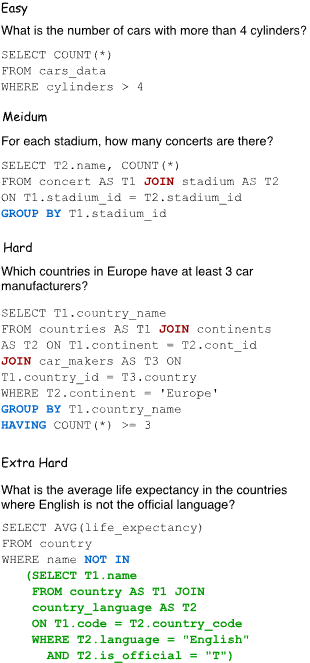
\includegraphics[width=0.35\textwidth]{image.png}
\caption{SQL query examples in 4 hardness levels. Credit: Spider [1]}
\label{fig:hardness-levels}
\end{figure}

\subsection{Prompting and Input}
\label{sec:prompting}

Each model receives three pieces of information in a single zero-shot user turn: a system instruction explaining its role as a Text-to-SQL generator, the database schema (table names, column names, primary keys, and foreign-key relationships, with no example rows), and the natural-language question. No few-shot examples are provided, so that the experiment measures each model's ability to generate SQL from instructions and schema information alone, without the confound of examples steering its output style. The prompt template is identical across all three models, so that differences in performance can be attributed to the models rather than to differences in prompting.

\textbf{Prompt template:}
\begin{verbatim}
Given the following SQLite database schema, write a SQL query that answers
the question.

{schema}

Question: {question}

Respond with only the SQL query in a ```sql code block.
\end{verbatim}

See \hyperref[sec:appendix1]{Appendix 1} for a worked example: a full schema, a question, and the resulting filled prompt.

\subsection{SQL Extraction}
\label{sec:sql-extraction}

For each sample, we decode the model's generated tokens into text using the model-specific tokenizer, and check for the presence of a \texttt{</think>} token. If \texttt{</think>} was generated, we take all text generated before \texttt{</think>} as the reasoning trace and all text to the right as the output SQL; DeepSeek-R1-Distill-Qwen-1.5B is the only model of the three that can emit this token. The SQL is then extracted from the first \texttt{```sql} code block in that remaining text. The extracted SQL is passed to the evaluation script as-is. Outputs that cannot be extracted or parsed are counted as incorrect on every metric rather than excluded from the evaluation, as unusable output is a task failure (see \ref{sec:evaluation-metrics} and \ref{sec:invalid-outputs}).

\subsection{Inference Settings}
\label{sec:inference-settings}

All models are evaluated using the same decoding configuration: greedy decoding (temperature and top-p are not applicable) for consistent, reproducible results between runs. The maximum output length differs by model: 256 tokens for Qwen3-0.6B, and 4096 tokens for both Qwen3-4B and DeepSeek-R1-Distill-Qwen-1.5B. For DeepSeek, the larger budget is needed because its output also has to contain a full reasoning trace rather than only the SQL query; Qwen3-4B is given the same, larger budget as DeepSeek so that a tighter token limit can be ruled out as the reason for any difference between them on invalid-output rate (\ref{sec:invalid-outputs}) or inference time (\ref{sec:efficiency}). Qwen3-0.6B and Qwen3-4B are both run with thinking mode off (both support it). DeepSeek-R1-Distill-Qwen-1.5B always produces a reasoning trace and has no documented way to disable thinking mode, so it is evaluated as the reasoning condition against the two non-reasoning Qwen3 models. All inference runs on the same 1x RTX 4090 GPU described in \ref{sec:models}, with batch size 1.

\subsection{Evaluation}
\label{sec:evaluation-metrics}

We evaluate the output using the same metrics as the Spider paper [1]. These are:

\begin{enumerate}
\item Component Matching
    \begin{itemize}
        \item For each of the following components:
        \begin{itemize}
            \item SELECT
            \item WHERE
            \item GROUP BY
            \item ORDER BY
            \item KEYWORDS (including all SQL keywords without column names and operators)
        \end{itemize}
        \item Decompose each component in the prediction and ground truth as bags of several sub-components and check whether or not these two sets of components match completely.
        \item Checks accuracy, recall, and F1
    \end{itemize}
\item Exact Matching Accuracy
    \begin{itemize}
        \item We measure whether the generated query as a whole is equivalent to the last section
        \item The generated query is correct only if all components are correct
        \item Checks only accuracy
    \end{itemize}
\item Execution Accuracy
    \begin{itemize}
        \item A list of gold values for each question is given
        \item We measure how many gold values the generated query extracts when executed
        \item Checks only accuracy
    \end{itemize}
\end{enumerate}

If output is invalid or unparsable, then it fails all 3 dimensions (component matching, exact matching, execution accuracy), consistent with how \ref{sec:sql-extraction} extracts and passes SQL to this evaluation script. This is reasonable as invalid/unparsable output cannot be applied to SQL and thus must be avoided and penalized heavily; Results~\ref{sec:invalid-outputs} reports how often this happens for each model.

\section{Task 1 -- RQ1: Results}
\label{sec:rq1-results}

\subsection{Overall Model Performance}
\label{sec:overall-performance}

Below we report how Qwen3-0.6B, Qwen3-4B, and Deepseek-R1-Distill-Qwen3-1.5B perform on the Spider benchmark across all 3 metrics (Component Matching, Exact Matching Accuracy, Execution Accuracy). We calculate the values per problem difficulty as well as overall, and display them in the below tables.

\begin{table}[H]
\centering
\footnotesize
\caption{Overall performance summary, aggregated across all difficulties (all 1034 problems). Component matching is accuracy / recall / F1 (macro-averaged, see the note on table~\ref{tab:difficulty-component} in \ref{sec:rq1-interpretation}). Per-difficulty breakdowns are in tables~\ref{tab:difficulty-component}--\ref{tab:difficulty-execution}.}
\label{tab:overall-performance}
\resizebox{\textwidth}{!}{%
\begin{tabular}{lllccc}
\toprule
Model & Parameters & Category & Component matching & Exact matching & Execution accuracy \\
\midrule
Qwen3-0.6B & 0.6B & Decoder-only & 0.628 / 0.209 / 0.314 & 0.099 & 0.209 \\
Qwen3-4B & 4B & Decoder-only & 0.797 / 0.306 / 0.442 & 0.256 & 0.353 \\
DeepSeek-R1-Distill-Qwen-1.5B & 1.5B & Reasoning & 0.661 / 0.174 / 0.275 & 0.085 & 0.121 \\
\bottomrule
\end{tabular}}
\end{table}

All models are evaluated zero-shot with the same prompt on the 20 databases of the Spider dev set. Aggregated across all difficulties and databases, every model is still far from solving the task: execution accuracy ranges from 0.121 (DeepSeek) to 0.353 (Qwen3-4B) and exact matching accuracy from 0.085 (DeepSeek) to 0.256 (Qwen3-4B). Execution accuracy is higher than exact matching accuracy for all three models (for example 0.353 vs.\ 0.256 for Qwen3-4B), which suggests that at least some of the queries that return the correct result are written differently from the gold SQL (see \ref{sec:rq1-interpretation} for more on this relationship). Of the three models, Qwen3-4B is now the best on almost every metric, database, and difficulty level; \ref{sec:by-database} and \ref{sec:rq1-interpretation} quantify how consistently. Table~\ref{tab:inference-time} reports the efficiency side of this comparison: inference time per example.

\subsection{Performance by Query Difficulty}
\label{sec:by-difficulty}

\begin{table}[H]
\centering
\footnotesize
\caption{Component matching (accuracy / recall / F1) by difficulty.}
\label{tab:difficulty-component}
\begin{tabular}{lcc}
\toprule
Model & easy & medium \\
\midrule
Problems (n) & 248 & 446 \\
Qwen3-0.6B & 0.675 / 0.308 / 0.423 & 0.582 / 0.235 / 0.334 \\
Qwen3-4B & 0.838 / 0.574 / 0.681 & 0.670 / 0.306 / 0.420 \\
DeepSeek-R1-Distill-Qwen-1.5B & 0.566 / 0.288 / 0.382 & 0.642 / 0.185 / 0.287 \\
\bottomrule
\end{tabular}

\vspace{0.5em}

\begin{tabular}{lccc}
\toprule
Model & hard & extra & all \\
\midrule
Problems (n) & 174 & 166 & 1034 \\
Qwen3-0.6B & 0.540 / 0.141 / 0.223 & 0.578 / 0.160 / 0.250 & 0.628 / 0.209 / 0.314 \\
Qwen3-4B & 0.796 / 0.262 / 0.394 & 0.485 / 0.150 / 0.229 & 0.797 / 0.306 / 0.442 \\
DeepSeek-R1-Distill-Qwen-1.5B & 0.543 / 0.113 / 0.187 & 0.389 / 0.104 / 0.164 & 0.661 / 0.174 / 0.275 \\
\bottomrule
\end{tabular}
\end{table}

\begin{table}[H]
\centering
\footnotesize
\caption{Exact matching accuracy by difficulty.}
\label{tab:difficulty-exact}
\begin{tabular}{lccccc}
\toprule
Model & easy & medium & hard & extra & all \\
\midrule
Problems (n) & 248 & 446 & 174 & 166 & 1034 \\
Qwen3-0.6B & 0.157 & 0.137 & 0.006 & 0.006 & 0.099 \\
Qwen3-4B & 0.508 & 0.262 & 0.115 & 0.012 & 0.256 \\
DeepSeek-R1-Distill-Qwen-1.5B & 0.214 & 0.078 & 0.000 & 0.000 & 0.085 \\
\bottomrule
\end{tabular}
\end{table}

\begin{table}[H]
\centering
\footnotesize
\caption{Execution accuracy by difficulty.}
\label{tab:difficulty-execution}
\begin{tabular}{lccccc}
\toprule
Model & easy & medium & hard & extra & all \\
\midrule
Problems (n) & 248 & 446 & 174 & 166 & 1034 \\
Qwen3-0.6B & 0.210 & 0.276 & 0.126 & 0.114 & 0.209 \\
Qwen3-4B & 0.565 & 0.345 & 0.276 & 0.139 & 0.353 \\
DeepSeek-R1-Distill-Qwen-1.5B & 0.258 & 0.128 & 0.017 & 0.006 & 0.121 \\
\bottomrule
\end{tabular}
\end{table}

We break every metric down by the Spider Hardness Criteria (\ref{sec:eval-data}) as query difficulty is a first-order driver of Text-to-SQL performance; comparing models only in aggregate would hide whether a model's advantage holds up as queries get harder.

Performance decreases with difficulty for every model, but the decrease is steepest for Qwen3-0.6B and DeepSeek: their exact matching and execution accuracy are both at most 0.034 and 0.126 respectively on hard and extra problems, down from as high as 0.210-0.258 (easy execution) on the easiest problems (table~\ref{tab:difficulty-exact} and table~\ref{tab:difficulty-execution}). Qwen3-4B degrades on the same relative scale but from a much higher starting point, from 0.508 easy exact matching / 0.565 easy execution accuracy down to 0.012 extra exact matching / 0.139 extra execution accuracy. Despite the degredation, it remains the best of the three models at every single difficulty level on both metrics (tables~\ref{tab:difficulty-exact}--\ref{tab:difficulty-execution}).

\subsection{Performance by Database}
\label{sec:by-database}

We also break execution and exact matching accuracy down by each of the 20 Spider dev databases. Qwen3-4B has the highest execution accuracy on 17 of the 20 databases outright (plus a tie on one more) and the highest exact matching accuracy on 18 of 20, while DeepSeek-R1-Distill-Qwen-1.5B is never highest on either metric; Qwen3-0.6B wins outright only on orchestra and battle\_death. Databases with few problems (real\_estate\_properties with n=4, voter\_1 with n=15, battle\_death with n=16, and museum\_visit with n=18) are too small to rank the models reliably, since a single problem changes a score by 6 to 25 percentage points. Execution accuracy ranges from 0.10 (course\_teach) to 0.53 (singer) for Qwen3-0.6B, from 0.19 (battle\_death) to 0.60 (singer) for Qwen3-4B, and from 0.00 (concert\_singer) to 0.27 (singer and voter\_1) for DeepSeek-R1-Distill-Qwen-1.5B (\hyperref[tab:db-execution]{Table 5}). The pattern on exact matching accuracy is just as one-sided (\hyperref[tab:db-exact]{Table 6}): Qwen3-4B is highest on 18 of 20 databases, ties Qwen3-0.6B on orchestra, and loses only on battle\_death; DeepSeek's exact matching accuracy is never the highest of the three, coming closest on flight\_2 (0.200 vs.\ Qwen3-4B's 0.350 and Qwen3-0.6B's 0.075). The full per-database tables and discussion are in \hyperref[sec:appendix2]{Appendix 2}.

\subsection{Invalid and Unparseable Outputs}
\label{sec:invalid-outputs}

We also count how often each model's output cannot be used as SQL at all: it either never produces a usable query within the token budget (\ref{sec:inference-settings}) or is truncated before finishing one. Per \ref{sec:evaluation-metrics}, these count as failures on every metric rather than being excluded, and this is a direct measure of how reliably each model follows the ``respond with only a SQL query'' instruction, independent of whether the SQL it does produce is correct. Qwen3-0.6B's invalid rate is 2.2\%, Qwen3-4B's is 0.0\%, and DeepSeek-R1-Distill-Qwen-1.5B's is 9.7\%, about 4x higher than Qwen3-0.6B's despite having the same 4096-token budget as Qwen3-4B (\ref{sec:inference-settings}), i.e. a larger token budget did not cause Qwen3-4B to run on or produce unusable output the way it does for DeepSeek. \ref{sec:rq1-interpretation} breaks DeepSeek's failures down further by difficulty and by why the generation failed (tables~\ref{tab:deepseek-outcome}--\ref{tab:deepseek-unfinished-by-difficulty}).

\subsection{Efficiency Measures}
\label{sec:efficiency}

\begin{table}[H]
\centering
\footnotesize
\caption{Output tokens per example}
\label{tab:tokens-per-example}
\begin{tabular}{lccccc}
\toprule
Model & easy & medium & hard & extra & all \\
\midrule
Qwen3-0.6B & 27.5 & 44.7 & 53.7 & 69.9 & 46.1 \\
Qwen3-4B & 23.6 & 37.3 & 46.2 & 59.0 & 39.0 \\
DeepSeek-R1-Distill-Qwen-1.5B & 610.8 & 768.4 & 1096.0 & 1176.9 & 851.3 \\
\bottomrule
\end{tabular}
\end{table}

Inference time is measured from the start of generation to the complete batch output, per batch of 1 example, excluding tokenization, model loading, and warm-up.

\begin{table}[H]
\centering
\footnotesize
\caption{Inference time.}
\label{tab:inference-time}
\begin{tabular}{lcc}
\toprule
Model & Total wall time (s) & Avg.\ time per example (s) \\
\midrule
Qwen3-0.6B & 123.9 & 0.120 \\
Qwen3-4B & 109.1 & 0.106 \\
DeepSeek-R1-Distill-Qwen-1.5B & 3059.8 & 2.959 \\
\bottomrule
\end{tabular}
\end{table}

DeepSeek is about 25x slower per example than Qwen3-0.6B and 28x slower than Qwen3-4B, consistent with its much higher average token count (table~\ref{tab:tokens-per-example}). Qwen3-4B, despite having about 7x as many parameters as Qwen3-0.6B, is marginally faster per example (0.106s vs.\ 0.120s), consistent with it generating fewer tokens on average (39.0 vs.\ 46.1, table~\ref{tab:tokens-per-example}) despite having the same 16x larger token budget as DeepSeek (\ref{sec:inference-settings}).

\begin{table}[H]
\centering
\footnotesize
\caption{DeepSeek-R1-Distill-Qwen-1.5B by generation outcome. ``Cut'' means the generation reached the 4096-token limit.}
\label{tab:deepseek-outcome}
\begin{tabular}{lccccc}
\toprule
Outcome & Problems (n) & Share & Avg.\ tokens & Exact match & Component F1 \\
\midrule
Finished with SQL & 934 & 90.3\% & 512 & 0.094 & 0.286 \\
Finished, no usable SQL & 2 & 0.2\% & 284 & 0.000 & 0.100 \\
Cut while answering (after \texttt{</think>}) & 13 & 1.3\% & 4096 & 0.000 & 0.096 \\
Cut while thinking (no \texttt{</think>}) & 85 & 8.2\% & 4096 & 0.000 & 0.093 \\
All & 1034 & 100\% & 851 & 0.085 & 0.275 \\
\bottomrule
\end{tabular}
\end{table}

\begin{table}[H]
\centering
\footnotesize
\caption{The same 934 questions that DeepSeek finished, for all three models.}
\label{tab:deepseek-finished-934}
\begin{tabular}{lcc}
\toprule
Model & Exact match & Component F1 \\
\midrule
DeepSeek-R1-Distill-Qwen-1.5B & 0.094 & 0.286 \\
Qwen3-0.6B & 0.103 & 0.317 \\
Qwen3-4B & 0.257 & 0.440 \\
\bottomrule
\end{tabular}
\end{table}

\begin{table}[H]
\centering
\footnotesize
\caption{Are the cut-off DeepSeek generations infinite self-repetition loops? A text that repeats itself compresses well, so a low compression ratio of the last 3000 characters indicates a loop.}
\label{tab:deepseek-repetition}
\begin{tabular}{lcccc}
\toprule
Generations & n & Median compression ratio & Ratio $<$ 0.15 & Last 150 characters repeat 3 or more times \\
\midrule
Cut off & 98 & 0.095 & 95.9\% & 96.9\% \\
Finished & 936 & 0.418 & 0.0\% & 0.2\% \\
\bottomrule
\end{tabular}
\end{table}

\begin{table}[H]
\centering
\footnotesize
\caption{Share of DeepSeek generations that did not finish with SQL, by difficulty.}
\label{tab:deepseek-unfinished-by-difficulty}
\begin{tabular}{lccccc}
\toprule
 & easy & medium & hard & extra & all \\
\midrule
Problems (n) & 248 & 446 & 174 & 166 & 1034 \\
Not finished with SQL (n) & 15 & 33 & 25 & 27 & 100 \\
Share & 6.0\% & 7.4\% & 14.4\% & 16.3\% & 9.7\% \\
\bottomrule
\end{tabular}
\end{table}

\section{Interpretation and Answer to Research Question (RQ1)}
\label{sec:rq1-interpretation}

\textbf{RQ1:} How do (selected) LLMs perform on cross-domain Text-to-SQL?

\vspace{10px}

All three models are still far from solving the task in this zero-shot setting: exact matching accuracy ranges from 0.085 to 0.256 and execution accuracy from 0.121 to 0.353 (table~\ref{tab:overall-performance}). Difficulty and database effects are discussed in \ref{sec:by-difficulty} and \ref{sec:by-database}; here we interpret the effects of model size and reasoning architecture and the exact-match/execution-accuracy relationship, and state the answer to RQ1 as three findings.

\textbf{First, within the Qwen family, scale is a strong and almost uniform predictor of performance, but an intermediate-size reasoning model from the Deepseek family still loses to the smallest model in the Qwen family.} Aggregated across all difficulties, Qwen3-4B has the best component matching (0.797 / 0.306 / 0.442), exact matching (0.256), and execution accuracy (0.353) of the three (table~\ref{tab:overall-performance}), and it beats Qwen3-0.6B on exact matching and execution accuracy at every individual difficulty level, including hard (0.115 vs.\ 0.006) and extra (0.012 vs.\ 0.006), where the smaller model solves almost nothing (tables~\ref{tab:difficulty-exact}--\ref{tab:difficulty-execution}). This is the largest, most consistent effect in the RQ1 results. The one exception is component matching on extra-hard problems, where Qwen3-0.6B's accuracy, recall, and F1 (0.578 / 0.160 / 0.250) are all slightly higher than Qwen3-4B's (0.485 / 0.150 / 0.229), the only point in the RQ1 results where the smaller Qwen3 model wins outright (table~\ref{tab:difficulty-component}). DeepSeek-R1-Distill-Qwen-1.5B sits between the two Qwen3 models in parameter count (1.5B) and is the only one that reasons, yet it is the lowest of the three on every aggregate metric (0.275 component F1, 0.085 exact matching, 0.121 execution accuracy) except its own component-matching accuracy (0.661 vs.\ 0.628 for Qwen3-0.6B). Thus, scale predicts performance well within a family, but does not transfer across the reasoning/non-reasoning boundary: having more parameters than Qwen3-0.6B did not help DeepSeek catch up to it.

\textbf{Second, the reasoning architecture itself, not parameter count, is the main driver of DeepSeek's low score.} Its invalid-output rate (9.7\%) is markedly higher than Qwen3-0.6B's (2.2\%) and Qwen3-4B's (0.0\% in this run) (\ref{sec:invalid-outputs}). In tables~\ref{tab:deepseek-outcome}--\ref{tab:deepseek-unfinished-by-difficulty}, 100 of 1034 generations (9.7\%) end without usable SQL. 85 never leave the reasoning phase, 13 are cut while writing the answer, and 2 finish without SQL. The number of unusable SQL generations also grows with difficulty, from 6.0\% on easy to 16.3\% on extra problems. These are not cases of long productive reasoning either: 95.9\% of the cut-off generations are highly self-repetitive (compression ratio below 0.15, median compression ratio 0.095, vs.\ 0.418 for finished generations), rewriting the same query and repeating phrases like ``So the final query is:'' without converging. Finishing does not make it better either: on the 934 questions DeepSeek does finish, its exact matching (0.094) and component F1 (0.286) are still below Qwen3-0.6B's on the same questions (0.103 / 0.317) and far below Qwen3-4B's (0.257 / 0.440), despite generating 512 tokens per question on average there, against 46 and 39 tokens overall for Qwen3-0.6B and Qwen3-4B (about 18x and 22x fewer). This extra length also costs time: DeepSeek is 25-28x slower per example than either Qwen3 model (\ref{sec:efficiency}). The reasoning trace mostly lengthens the output and sometimes never terminates, without improving the SQL when it does, and size alone is not the explanation, since Qwen3-4B is both bigger than DeepSeek and the best model in the comparison. Thus, reasoning architecture itself, not the parameter count, is the main driver of DeepSeek's low score.

\textbf{Third, query difficulty has a substantial, consistent effect on every model, including the best one.} Exact matching and execution accuracy both fall sharply from easy to extra-hard problems for all three models (\ref{sec:by-difficulty}). Qwen3-4B's drop is from a much higher base (0.508 to 0.012 exact matching, 0.565 to 0.139 execution accuracy) and it remains the best model at every difficulty level on both metrics, but the drop itself is just as steep in relative terms as for the other two models, and the hardest problems remain largely unsolved even for it.

\textbf{Exact match vs.\ execution accuracy.} For all three models, execution accuracy aggregated across all difficulties exceeds exact matching accuracy (table~\ref{tab:overall-performance}): 0.209 vs.\ 0.099 for Qwen3-0.6B, 0.353 vs.\ 0.256 for Qwen3-4B, and 0.121 vs.\ 0.085 for DeepSeek. Since exact matching requires every SQL component to match the gold query while execution accuracy only requires the same result set, this gap indicates each model writes some queries that are valid and correct but phrased differently from the gold SQL (e.g.\ a different but equivalent join order, or an explicit column list where the gold query uses \texttt{SELECT *}). The gap is widest for Qwen3-0.6B (11.0 points), close behind for Qwen3-4B (9.7 points), and narrowest for DeepSeek (3.6 points); DeepSeek's narrower gap reflects it producing fewer alternative-but-valid queries. Qwen3-4B's gap is almost as wide as Qwen3-0.6B's despite much higher absolute accuracy, so scaling up within the Qwen3 family raises both Exact Match Accuracy and Execution Accuracy together rather than closing the gap between them.

\textbf{Limitations.} Our working hypothesis is that Text-to-SQL at this scale does not benefit from an explicit reasoning trace, and that a non-reasoning model is sufficient, with performance instead scaling with parameter count within a fixed model family. The results are consistent with this hypothesis. However, they do not establish that Text-to-SQL is too simple for reasoning models in general due to several factors:

\begin{itemize}
\item \textbf{Truncation and failed outputs for DeepSeek.} These count as failures on every metric and lower its recall, exact matching, and execution scores, but table~\ref{tab:deepseek-finished-934} shows removing them would not change the ranking (DeepSeek is also lower on the questions it finished), and table~\ref{tab:deepseek-repetition} shows the cut-off generations are repetition loops, so a larger token budget is unlikely to rescue them.
\item \textbf{Model differences beyond reasoning.} Qwen3-0.6B and Qwen3-4B share a model family, isolating the effect of scale between them, but DeepSeek differs from both in family, size, and pretraining/post-training, not only in whether it reasons; it is also a distilled model, so the effect of reasoning cannot be fully separated from distillation quality.
\item \textbf{Aggregated component matching.} The component matching figures in table~\ref{tab:difficulty-component} (and in table~\ref{tab:overall-performance}) are our own macro-average (mean of the 10 per-component accuracy and recall scores, with F1 computed from these two means), not a number reported by Spider.
\end{itemize}

Overall, in this zero-shot, cross-domain setting, a larger non-reasoning decoder-only model (Qwen3-4B, 4B) clearly outperforms both a same-family model at under a sixth its size (Qwen3-0.6B) and a reasoning model of intermediate size from a different family (DeepSeek-R1-Distill-Qwen-1.5B, 1.5B), while also being faster per example than either. None of the three models solve more than half of even the easiest problems or more than a small fraction of hard or extra-hard queries. This answers RQ1 for the three models evaluated.
 (this
% file's cross-references into Task 1 -- table~\ref{tab:deepseek-outcome},
% \ref{tab:tokens-per-example}, \ref{sec:sql-extraction}, etc. -- rely on
% RQ1.tex's labels already being defined earlier in the same document).
%
% Structure: Methodology is organized per-feature (Feature 1: Token Count,
% Feature 2: Information Retention), each with its own Definition / Why it's
% relevant / How we computed it. Results is organized as descriptive
% statistics, differences by correctness, differences by difficulty, and
% relationship with Text-to-SQL correctness (the correlation analysis).

\section{Task 2 -- RQ2: Methodology}
\label{sec:rq2-methodology}

\textbf{RQ2:} How do characteristics of reasoning traces (of reasoning LLM) relate to Text-to-SQL performance?

To answer this question, we examine two features of each reasoning trace: Token Count and Information Retention. We compute both for all 1034 generations in DeepSeek-R1-Distill-Qwen-1.5B's main Task 1 run, then relate each to difficulty and to Text-to-SQL correctness.

\subsection{Feature 1: Token Count}
\label{sec:rq2-feature-tokencount}

\textbf{Definition.} Token Count is the number of tokens in the reasoning segment of a generation, i.e.\ everything the model generates before \texttt{</think>}, excluding the final SQL answer. We split each generation into a reasoning segment and an answer segment using the same \texttt{</think>} split used in Task 1 (\ref{sec:sql-extraction}).

\textbf{Why it's relevant.} We expect Token Count to scale positively with the difficulty of the related Text-to-SQL problem: easy questions should require fewer thinking tokens, while extra-hard questions should require significantly more. Any question that disobeys this relation, or where more tokens associate with worse rather than better answers, is given special attention in Results. Token Count is also the most direct, model-agnostic proxy we have for how much deliberation went into an answer, so it is a natural first feature to test against correctness.

\textbf{How we computed it.} Token Count is the number of tokens in the reasoning segment only, re-tokenized with the model's own tokenizer (not the \texttt{new\_tokens} field logged during generation, which counts the whole generation, reasoning plus SQL). For generations that never emit \texttt{</think>} (truncated at the 4096-token generation limit, see Task 1's table~\ref{tab:deepseek-outcome}), the entire generated text is treated as the reasoning segment, so Token Count for these rows is effectively capped at the generation limit rather than reflecting a completed thought. This is intentional: these cases are exactly the repetition loops Task 1 identified (table~\ref{tab:deepseek-repetition}), and dropping them would hide, rather than explain, the heavy right tail in Token Count. We keep them in the Token Count analysis and flag wherever they drive a result (see finding~\ref{item:rq2-finding-tokencount-difficulty} in Results).

\begin{table}[H]
\centering
\footnotesize
\caption{Token Count: definition and computation summary.}
\label{tab:rq2-feature-tokencount-summary}
\begin{tabular}{p{0.22\textwidth}p{0.7\textwidth}}
\toprule
Property & Detail \\
\midrule
Unit & Tokens (model's own tokenizer) \\
Scope & Reasoning segment only, i.e.\ text before \texttt{</think>} \\
Range & Non-negative integer, long right tail (observed 103--4166) \\
Truncated traces & Treated as reasoning segment in full; capped at the 4096-token generation limit \\
Hypothesis & Increases with difficulty; should not correlate with worse correctness \\
Test & Spearman's rank correlation vs.\ difficulty and vs.\ 32 per-question performance submetrics \\
\bottomrule
\end{tabular}
\end{table}

\subsection{Feature 2: Information Retention}
\label{sec:rq2-feature-retention}

\textbf{Definition.} Information Retention is the share of schema-shaped identifiers mentioned in a reasoning trace that actually exist as a table or column name in that question's schema. Equivalently, $1 - $ Information Retention is the hallucination rate of the trace: the fraction of mentioned identifiers that are not grounded in the prompt.

\textbf{Why it's relevant.} We expect reasoning traces with low Information Retention (frequent hallucination of schema elements) to produce lower-performing answers than traces that stay grounded in the given schema, since inventing a table or column that doesn't exist is very likely to propagate into an incorrect query. We also expect harder problems to not cause lower Information Retention on their own; if they do, this points to the model introducing more assumptions as questions get harder, which is itself worth investigating as a bias rather than attributing the accuracy drop to difficulty alone.

\textbf{How we computed it.} We regex-extract every schema-shaped identifier the trace mentions, either quoted (e.g.\ \texttt{"Singer\_ID"}) or underscore-joined (e.g.\ \texttt{concert\_id}), and take the share of those identifiers that match a table or column name in that question's schema. An identifier that matches neither is treated as a fact the model introduced on its own, i.e., a hallucination. Traces that mention no schema identifiers at all are excluded from Information Retention (but kept for Token Count), since a 0-of-0 ratio is undefined rather than evidence of perfect or zero retention; this drops the usable sample from 1034 to 1017. Truncated traces are scored the same way, over whatever partial text was generated.

\begin{table}[H]
\centering
\footnotesize
\caption{Information Retention: definition and computation summary.}
\label{tab:rq2-feature-retention-summary}
\begin{tabular}{p{0.22\textwidth}p{0.7\textwidth}}
\toprule
Property & Detail \\
\midrule
Unit & Ratio, bounded in $[0,1]$ \\
Numerator & Schema identifiers mentioned in the trace that match a real table/column name \\
Denominator & All schema-shaped identifiers mentioned in the trace (quoted or underscore-joined) \\
Exclusions & Traces mentioning zero schema identifiers (1034 $\rightarrow$ 1017 usable rows) \\
Truncated traces & Scored over the partial text generated before truncation \\
Hypothesis & Higher retention associates with better correctness; should not fall with difficulty \\
Test & Spearman's rank correlation vs.\ difficulty and vs.\ 32 per-question performance submetrics \\
\bottomrule
\end{tabular}
\end{table}

\subsection{Statistical approach}
\label{sec:rq2-statistical-approach}

We relate both Token Count and Information Retention to correctness and difficulty with Spearman's Rank Correlation throughout. Both of our hypotheses are about monotonic relationships, not linear relationships (performance should not decrease as Token Count or Information Retention increase, and Token Count should increase with difficulty), which is exactly what Spearman's Rank Correlation tests for. It also suits the distribution of our two reasoning metrics: Token Count is a non-negative count with a long right tail (DeepSeek alone ranges from 611 tokens on easy problems to 1177 on extra, table~\ref{tab:tokens-per-example}), and Information Retention is a bounded ratio, so neither is likely to be symmetric and unbounded; the $\geq$90\% trace completion rate gives us enough data per stratum to check this on histograms rather than assume it. For correctness, we correlate each reasoning metric against the continuous, per-question component matching accuracy, recall, and F1 for all ten Spider components individually, plus exact matching and execution accuracy, rather than collapsing them into one pass/fail label, which keeps the per-question variance in performance a binary cutoff would discard and sidesteps splitting by correctness directly, which is not viable per difficulty level: DeepSeek's exact matching accuracy falls to at most 0.034 on hard and extra problems, leaving as few as four to six correct traces in those strata. This gives 32 submetrics per reasoning metric per difficulty level. We chose this rank-based, continuous-correlation approach over a parametric correlation or a correct/incorrect group comparison because our data is too skewed for the former and our correct-answer strata too sparse for the latter. With 169 correlation tests run in total, we correct for multiple comparisons with the Benjamini-Hochberg procedure rather than a stricter family-wise correction like Bonferroni: we are screening many related, non-independent submetrics for the strongest associations to report and discuss, not making a small number of pre-registered confirmatory claims, so controlling the expected false-discovery rate is a better fit than controlling the probability of any single false positive at the cost of statistical power.

The Results below report Token Count and Information Retention broken down two ways: by difficulty, since that is the primary hypothesis under test, and by exact-match correctness (correct/incorrect), used for the descriptive statistics and the boxplots (figure~\ref{fig:rq2-boxplots}) because a binary split is easier to read in a table or figure than 32 continuous submetrics. The correlation analysis itself (table~\ref{tab:rq2-correlations}) still uses the continuous submetrics described above, for the statistical-power reasons given there; the binary-correctness view and the continuous-submetric view are two presentations of the same underlying data, not two different analyses.

\textbf{Verification.} To check that the Spearman findings above are not artifacts of one particular rank-based method or of an unmodeled confound, we add two further layers of testing, reported in \ref{sec:rq2-verification} and \ref{sec:rq2-robustness}. First, we run two confirmatory, feature-specific significance tests directly on the binary/ordinal views used for the descriptive statistics: a Mann-Whitney U test for each feature against exact-match correctness (overall and within each difficulty stratum), and Kendall's tau-b for each feature against difficulty (overall and within each correctness stratum). We prefer Kendall's tau-b over a second Spearman run here because it is the standard choice when one variable has many ties (difficulty has only four distinct values, and Information Retention has a large tied mass at 1.0), and it is the ordered-groups analogue of the Jonckheere-Terpstra trend test. Second, because Token Count, Information Retention and difficulty are all correlated with one another, a bivariate relationship between one feature and an outcome could simply be riding on the other two variables rather than reflecting an independent association. We fit two regression models to check this: a logistic regression of exact-match correctness on standardized log Token Count, standardized Information Retention, and standardized difficulty, all entered jointly; and a proportional-odds (ordinal) regression of difficulty on standardized log Token Count and standardized Information Retention, entered jointly. Token Count is log-transformed before standardizing given its heavy right skew (see above); difficulty enters the logistic model as a single linear control on the log-odds scale, which is a simplification rather than a full categorical treatment, and the ordinal model assumes proportional odds across the three difficulty thresholds, which we did not separately test -- both are limitations of this robustness check, not of the primary Spearman analysis. All four verification tests and both regression models are implemented in \texttt{eval/evalpipeline/reasoning\_verification.py}, run on the same per-question table as the Spearman analysis.

\section{Task 2 -- RQ2: Results}
\label{sec:rq2-results}

We compute Token Count and Information Retention for all 1034 generations in DeepSeek-R1-Distill-Qwen-1.5B's main Task 1 run, and correlate each against difficulty and against all 32 per-question performance submetrics as described in the Methodology. Table~\ref{tab:rq2-descriptive-stats-tokencount} and table~\ref{tab:rq2-descriptive-stats-retention} give descriptive statistics for each feature by difficulty and by exact-match correctness; figure~\ref{fig:rq2-boxplots} shows the resulting distributions; table~\ref{tab:rq2-correlations} lists the strongest correlations.

\subsection{Descriptive statistics}
\label{sec:rq2-descriptive-stats}

\begin{table}[H]
\centering
\footnotesize
\caption{Token Count descriptive statistics, by difficulty and by exact-match correctness (1 = exact match, 0 = not). Full results in \texttt{eval/results/task2\_analysis/descriptive\_stats.csv}.}
\label{tab:rq2-descriptive-stats-tokencount}
\begin{tabular}{lcccccc}
\toprule
Group & n & mean & median & std & min & max \\
\midrule
easy & 248 & 542.3 & 329.0 & 845.2 & 103 & 4096 \\
medium & 446 & 648.2 & 374.0 & 925.7 & 191 & 4166 \\
hard & 174 & 939.2 & 425.0 & 1246.2 & 226 & 4096 \\
extra & 166 & 901.6 & 434.5 & 1199.9 & 222 & 4096 \\
\midrule
exact match = 0 & 946 & 748.1 & 394.0 & 1065.6 & 103 & 4166 \\
exact match = 1 & 88 & 329.3 & 314.5 & 97.7 & 195 & 849 \\
\midrule
all & 1034 & 712.4 & 383.0 & 1026.2 & 103 & 4166 \\
\bottomrule
\end{tabular}
\end{table}

\begin{table}[H]
\centering
\footnotesize
\caption{Information Retention descriptive statistics, by difficulty and by exact-match correctness (1 = exact match, 0 = not). Excludes traces that mention no schema identifiers (n drops from 1034 to 1017 overall). Full results in \texttt{eval/results/task2\_analysis/descriptive\_stats.csv}.}
\label{tab:rq2-descriptive-stats-retention}
\begin{tabular}{lcccccc}
\toprule
Group & n & mean & median & std & min & max \\
\midrule
easy & 246 & 0.915 & 1.0 & 0.146 & 0.0 & 1.0 \\
medium & 441 & 0.905 & 1.0 & 0.148 & 0.0 & 1.0 \\
hard & 172 & 0.877 & 1.0 & 0.163 & 0.0 & 1.0 \\
extra & 158 & 0.861 & 1.0 & 0.215 & 0.0 & 1.0 \\
\midrule
exact match = 0 & 931 & 0.893 & 1.0 & 0.166 & 0.0 & 1.0 \\
exact match = 1 & 86 & 0.924 & 1.0 & 0.123 & 0.5 & 1.0 \\
\midrule
all & 1017 & 0.896 & 1.0 & 0.163 & 0.0 & 1.0 \\
\bottomrule
\end{tabular}
\end{table}

\begin{figure}[H]
\centering
\includegraphics[width=0.95\textwidth]{boxplots.png}
\caption{Token Count and Information Retention by difficulty and by exact-match correctness, for DeepSeek-R1-Distill-Qwen-1.5B's 1034 Task 1 generations. Green triangles are means, orange lines are medians. Means sit well above medians throughout, confirming the right-skewed, bounded distributions the Methodology assumes rather than normal ones.}
\label{fig:rq2-boxplots}
\end{figure}

\subsection{Differences by correctness}
\label{sec:rq2-by-correctness}

Correct generations (exact match = 1) have a much lower mean and tighter spread of Token Count (329.3, std 97.7) than incorrect ones (748.1, std 1065.6, table~\ref{tab:rq2-descriptive-stats-tokencount}), and a slightly higher mean Information Retention (0.924 vs.\ 0.893, table~\ref{tab:rq2-descriptive-stats-retention}). Both differences point the same direction as the correlation findings in \ref{sec:rq2-relationship-correctness}: more reasoning tokens and lower retention associate with worse performance. The gap is far larger for Token Count than for Information Retention: incorrect generations' Token Count std (1065.6) is more than ten times that of correct generations (97.7), driven by the truncated, repetition-loop traces described in \ref{sec:rq2-feature-tokencount}, almost none of which are exact matches. Information Retention's median is 1.0 in both correctness groups, so the correctness gap in retention lives entirely in the mean and the lower tail, not in a shift of the typical trace.

\subsection{Differences by difficulty}
\label{sec:rq2-by-difficulty}

\begin{enumerate}
\item \label{item:rq2-finding-tokencount-difficulty} \textbf{Token Count increases with difficulty, as hypothesized, but the increase is driven by a heavy tail.} Median token count rises from 329 (easy) to 374 (medium) to 425 (hard) to 434 (extra), and the correlation with difficulty is positive and significant ($\rho=0.313$, $q<0.001$). The mean rises faster than the median at every level (for example 542 vs.\ 329 on easy), because generations hitting the 4096-token limit occur at every difficulty (figure~\ref{fig:rq2-boxplots}, top row); these are the same repetition loops Task 1 identified, not productive extra reasoning on harder problems.
\item \label{item:rq2-finding-retention-difficulty} \textbf{Information Retention decreases slightly with difficulty.} Median retention is 1.0 at every difficulty level, but the mean falls from 0.915 (easy) to 0.861 (extra), and the correlation with difficulty is negative and significant ($\rho=-0.107$, $q=0.013$). Per the Methodology, this is the case that calls for examining the model's introduced assumptions on harder problems rather than attributing the accuracy drop to difficulty alone.
\end{enumerate}

\subsection{Relationship with Text-to-SQL correctness}
\label{sec:rq2-relationship-correctness}

\begin{enumerate}
\item \label{item:rq2-finding-tokencount-disobey} \textbf{On easy and medium problems, more Token Count tracks worse performance, the ``disobeying'' case flagged in the Methodology.} Token Count correlates negatively with \texttt{keywords} F1 on easy ($\rho=-0.42$, $q<0.001$) and medium ($\rho=-0.19$, $q=0.001$) problems, and with \texttt{where} and \texttt{where(no OP)} F1 on easy problems ($\rho=-0.32$ and $-0.33$, $q<0.001$). Combined with finding~\ref{item:rq2-finding-tokencount-difficulty}, the extra tokens on these problems look like run-away generation rather than helpful deliberation.
\item \label{item:rq2-finding-retention-performance} \textbf{Where Information Retention does relate to performance, it is positive, as hypothesized.} On medium problems, Information Retention correlates positively with \texttt{where} and \texttt{where(no OP)} F1 ($\rho=0.345$, $q<0.001$ for both), consistent with higher-retention traces producing more accurate WHERE clauses. Of the 169 tests run, 26 remain significant after Benjamini-Hochberg correction; the strongest are in table~\ref{tab:rq2-correlations}.
\end{enumerate}

\begin{table}[H]
\centering
\footnotesize
\caption{Strongest Spearman correlations between reasoning metrics and performance submetrics, Benjamini-Hochberg corrected, top 8 of 169 tests by q-value. Full results in \texttt{eval/results/task2\_analysis/spearman\_correlations.csv}.}
\label{tab:rq2-correlations}
\begin{tabular}{llcccc}
\toprule
Metric & Submetric & Difficulty & n & $\rho$ & $q$ \\
\midrule
Token Count & difficulty (overall) & all & 1034 & 0.313 & $<$0.001 \\
Information Retention & where F1 & medium & 441 & 0.345 & $<$0.001 \\
Information Retention & where(no OP) F1 & medium & 441 & 0.345 & $<$0.001 \\
Token Count & keywords F1 & easy & 248 & -0.417 & $<$0.001 \\
Token Count & where(no OP) F1 & easy & 248 & -0.332 & $<$0.001 \\
Token Count & where F1 & easy & 248 & -0.322 & $<$0.001 \\
Token Count & keywords F1 & medium & 446 & -0.194 & $<$0.001 \\
Information Retention & difficulty (overall) & all & 1017 & -0.107 & 0.013 \\
\bottomrule
\end{tabular}
\end{table}

\subsection{Verification: Mann-Whitney U and Kendall's tau-b}
\label{sec:rq2-verification}

\begin{table}[H]
\centering
\footnotesize
\caption{Mann-Whitney U test: Token Count by exact-match correctness, overall and within each difficulty stratum. $r$ is the rank-biserial correlation (negative = higher Token Count associates with incorrect answers). Full results in \texttt{eval/results/task2\_analysis/mann\_whitney\_tokencount.csv}.}
\label{tab:rq2-mw-tokencount}
\begin{tabular}{lccccc}
\toprule
Stratum & n(incorrect) & n(correct) & $U$ & $p$ & $r$ \\
\midrule
all & 946 & 88 & 60406.5 & $<$0.001 & -0.451 \\
easy & 195 & 53 & 6423.0 & 0.007 & -0.243 \\
medium & 411 & 35 & 9644.0 & 0.001 & -0.341 \\
hard & 174 & 0 & --- & --- & --- \\
extra & 166 & 0 & --- & --- & --- \\
\bottomrule
\end{tabular}
\end{table}

\begin{table}[H]
\centering
\footnotesize
\caption{Mann-Whitney U test: Information Retention by exact-match correctness, overall and within each difficulty stratum. Full results in \texttt{eval/results/task2\_analysis/mann\_whitney\_retention.csv}.}
\label{tab:rq2-mw-retention}
\begin{tabular}{lccccc}
\toprule
Stratum & n(incorrect) & n(correct) & $U$ & $p$ & $r$ \\
\midrule
all & 931 & 86 & 36583.5 & 0.136 & 0.086 \\
easy & 194 & 52 & 5245.0 & 0.601 & -0.040 \\
medium & 407 & 34 & 5989.0 & 0.137 & 0.134 \\
hard & 172 & 0 & --- & --- & --- \\
extra & 158 & 0 & --- & --- & --- \\
\bottomrule
\end{tabular}
\end{table}

\begin{table}[H]
\centering
\footnotesize
\caption{Kendall's tau-b: Token Count vs.\ difficulty, overall and within each correctness stratum. Full results in \texttt{eval/results/task2\_analysis/kendall\_tokencount.csv}.}
\label{tab:rq2-kendall-tokencount}
\begin{tabular}{lccc}
\toprule
Group & n & $\tau_b$ & $p$ \\
\midrule
all & 1034 & 0.239 & $<$0.001 \\
incorrect & 946 & 0.207 & $<$0.001 \\
correct & 88 & 0.130 & 0.141 \\
\bottomrule
\end{tabular}
\end{table}

\begin{table}[H]
\centering
\footnotesize
\caption{Kendall's tau-b: Information Retention vs.\ difficulty, overall and within each correctness stratum. Full results in \texttt{eval/results/task2\_analysis/kendall\_retention.csv}.}
\label{tab:rq2-kendall-retention}
\begin{tabular}{lccc}
\toprule
Group & n & $\tau_b$ & $p$ \\
\midrule
all & 1017 & -0.091 & $<$0.001 \\
incorrect & 931 & -0.093 & $<$0.001 \\
correct & 86 & 0.110 & 0.279 \\
\bottomrule
\end{tabular}
\end{table}

Token Count's relationship with correctness is confirmed by the Mann-Whitney test: the overall gap is highly significant ($p<0.001$) with a moderate rank-biserial effect ($r=-0.451$), and it holds up within both the easy ($p=0.007$) and medium ($p=0.001$) strata individually. Hard and extra cannot be tested at all, because this run has zero exact matches in either stratum (table~\ref{tab:rq2-mw-tokencount}) -- a direct, concrete confirmation of the Methodology's reason for using continuous correlation instead of a correctness split per difficulty level. Information Retention's correctness gap, by contrast, is \emph{not} statistically significant overall ($p=0.136$, table~\ref{tab:rq2-mw-retention}): the descriptive mean difference noted in \ref{sec:rq2-by-correctness} (0.924 vs.\ 0.893) is not large enough relative to the within-group spread to rule out chance at this sample size.

Kendall's tau-b replicates the Spearman difficulty trend for both features using a method that does not rely on an equal-interval difficulty scale and is designed for heavily tied data: Token Count's $\tau_b=0.239$ ($p<0.001$) is consistent in sign and significance with its Spearman $\rho=0.313$, and Information Retention's $\tau_b=-0.091$ ($p<0.001$) is consistent with its Spearman $\rho=-0.107$ (tables~\ref{tab:rq2-kendall-tokencount}--\ref{tab:rq2-kendall-retention}). Both trends replicate within the much larger incorrect stratum (931--946 rows) but are not significant within the sparse correct stratum (86--88 rows, $p=0.141$ and $0.279$), which is expected given the large drop in sample size rather than evidence against the trend.

\subsection{Robustness: controlling for confounds}
\label{sec:rq2-robustness}

\begin{table}[H]
\centering
\footnotesize
\caption{Logistic regression: exact match on standardized log Token Count, standardized Information Retention, and standardized difficulty, fit jointly ($n=1017$, pseudo $R^2=0.188$). OR is the odds ratio per one-SD increase in the predictor. Full results in \texttt{eval/results/task2\_analysis/logistic\_regression.csv}.}
\label{tab:rq2-logistic}
\begin{tabular}{lccccc}
\toprule
Predictor & coef & SE & $z$ & $p$ & OR [95\% CI] \\
\midrule
Intercept & -3.351 & 0.227 & -14.76 & $<$0.001 & 0.035 [0.022, 0.055] \\
log Token Count ($z$) & -1.087 & 0.300 & -3.62 & $<$0.001 & 0.337 [0.187, 0.607] \\
Information Retention ($z$) & 0.091 & 0.139 & 0.65 & 0.514 & 1.095 [0.834, 1.437] \\
Difficulty ($z$) & -1.278 & 0.201 & -6.35 & $<$0.001 & 0.279 [0.188, 0.413] \\
\bottomrule
\end{tabular}
\end{table}

\begin{table}[H]
\centering
\footnotesize
\caption{Proportional-odds (ordinal) regression: difficulty on standardized log Token Count and standardized Information Retention, fit jointly ($n=1017$). OR is the odds ratio per one-SD increase in the predictor. Full results in \texttt{eval/results/task2\_analysis/ordinal\_regression.csv}.}
\label{tab:rq2-ordinal}
\begin{tabular}{lccccc}
\toprule
Predictor & coef & SE & $z$ & $p$ & OR [95\% CI] \\
\midrule
log Token Count ($z$) & 0.398 & 0.059 & 6.78 & $<$0.001 & 1.489 [1.327, 1.670] \\
Information Retention ($z$) & -0.177 & 0.059 & -2.99 & 0.003 & 0.837 [0.746, 0.941] \\
\bottomrule
\end{tabular}
\end{table}

Controlling for the other feature and for difficulty changes which bivariate relationship survives. Token Count's association with correctness holds up: each one-SD increase in log Token Count is associated with 66\% lower odds of an exact match (OR$=0.337$, $p<0.001$), holding Information Retention and difficulty fixed (table~\ref{tab:rq2-logistic}) -- consistent with, and strengthening, finding~\ref{item:rq2-finding-tokencount-disobey}. Information Retention's association with correctness does not survive the same control (OR$=1.095$, $p=0.514$): once Token Count and difficulty are accounted for, Retention has no detectable independent effect on correctness, so the positive finding in \ref{item:rq2-finding-retention-performance} should be read as a submetric-specific, not a global, relationship. Both features' difficulty relationships, in contrast, are independent of one another: the ordinal regression finds Token Count still predicts higher difficulty (OR$=1.489$ per SD, $p<0.001$) and Information Retention still predicts lower difficulty (OR$=0.837$ per SD, $p=0.003$) when controlling for each other (table~\ref{tab:rq2-ordinal}), so neither difficulty trend in \ref{sec:rq2-by-difficulty} is simply a byproduct of the other feature's trend.
 into REPORT.tex, after % RQ1.tex -- Task 1 / RQ1 section, factored out of REPORT.tex.
%
% Intended use: % RQ1.tex -- Task 1 / RQ1 section, factored out of REPORT.tex.
%
% Intended use: % RQ1.tex -- Task 1 / RQ1 section, factored out of REPORT.tex.
%
% Intended use: \input{RQ1.tex} into REPORT.tex in place of the current inline
% "Task 1 -- RQ1: Methodology & Results" / "Task 1 -- RQ1: Results" content.
% REPORT.tex already loads every package this fragment needs (booktabs, array,
% graphicx, float, caption, hyperref), so no extra preamble is required.
%
% Annotations made while converting this to reference-based numbering:
%  - All \subsection*{N.M ...} / \section*{...} became real, numbered
%    \section/\subsection commands with the leading "N.M" stripped from the
%    title text (LaTeX now generates it), each with a \label. The former
%    \subsection*{3. Interpretation...} is promoted to a top-level \section,
%    since it was already numbered as a peer of Parts 1 and 2, not a child
%    of Part 2.
%  - Every table/figure got a \label right after its \caption, and every
%    in-text "table 1", "tables 2-4", "2.2", "Appendix 2", etc. became a
%    \ref (or \hyperref for Appendix 2/3, which live outside this file --
%    see note below). Because the Models table (1.1) is now counted and the
%    Appendix 2/3 tables are not part of this file's sequential numbering,
%    the printed table numbers shift versus the pasted draft (e.g. "table 1"
%    -> Table 2, "table 8" -> Table 6); every mention uses \ref, so this is
%    self-consistent and will stay correct if tables move again.
%  - Fixed a leftover inconsistency in 1.5: the draft's 1.1 and 2.5 both
%    state batch size 1 (confirmed correct), but 1.5 still said "batch size
%    128" (leftover from an earlier draft) -- corrected to 1.
%  - Both TODOs in the pasted draft are resolved inline: 2.2 now cites
%    Tables 4-5 directly instead of a placeholder, and 2.3 now cites the
%    concrete per-database numbers from Appendix 2 (pulled from REPORT.tex's
%    existing Appendix 2 prose) instead of a placeholder.
%  - The Overall Performance table's caption promises "the note on table 2
%    in 3" (i.e. a note about macro-averaged component matching, to appear
%    in the Interpretation section), but the pasted draft's Limitations list
%    dropped that bullet (it only kept "Truncation" and "Model differences").
%    Restored the "Aggregated component matching" bullet from the prior
%    REPORT.tex draft so the caption's forward reference resolves to real
%    content; this is a content restoration, not just a labeling change,
%    so flagging it here. The other previously-present bullet ("Single run
%    and sample size") was NOT restored, since nothing in the new draft
%    points to it -- worth confirming with the author whether that drop was
%    intentional.
%  - Appendix 1/2/3 and their tables (5, 6, 7) live in REPORT.tex, outside
%    this file. REPORT.tex's appendix tables keep their existing manual
%    "Table 5/6/7:" caption numbering (renumbering them would require
%    restructuring the whole document's table order, which is out of scope
%    here); \label{tab:db-execution}, \label{tab:db-exact} and
%    \label{tab:invalid-outputs} were added to those tables in REPORT.tex
%    (additive only, no visible change) so this file can link to them.
%    Since their printed numbers are not auto-generated, this file links to
%    them with \hyperref[label]{5}-style calls (a real clickable link, with
%    text matching the manual number already in their caption) rather than
%    \ref (which would print whatever their true document-order table
%    number is, not 5/6/7).

\section{Task 1 -- RQ1: Methodology \& Results}
\label{sec:rq1-methods}

\textbf{RQ1:} How do (selected) LLMs perform on cross-domain Text-to-SQL?

In this report we evaluate the performance of decoder-only language models as well as reasoning LLMs on cross-domain SQL.

\subsection{Models}
\label{sec:models}

We compare two decoder-only LLMs from the same model family at different scales (Qwen3-0.6B and Qwen3-4B) against one reasoning LLM, so that the comparison isolates the effect of scale within a fixed family from the effect of an explicit reasoning trace, as much as a 3-model study can. All three are accessed as local inference over their bf16 Huggingface checkpoints on 1x NVIDIA GeForce RTX 4090 GPU (no API-based models), so that inference parameters are fully under our control (see \ref{sec:inference-settings}). We evaluate using batch sizes of 1.

\begin{table}[H]
\centering
\footnotesize
\caption{Models compared in RQ1.}
\label{tab:models}
\resizebox{\textwidth}{!}{%
\begin{tabular}{llllll}
\toprule
Model & Category & Parameters & Quantization & Access & Thinking mode \\
\midrule
Qwen3-0.6B [2] & Decoder-only & 0.6B & bf16 (none beyond release precision) & Local, Huggingface checkpoint & Disabled \\
Qwen3-4B [2] & Decoder-only & 4B & bf16 (none beyond release precision) & Local, Huggingface checkpoint & Disabled \\
DeepSeek-R1-Distill-Qwen-1.5B [4] & Reasoning & 1.5B & bf16 (none beyond release precision) & Local, Huggingface checkpoint & Always on (no disable option) \\
\bottomrule
\end{tabular}}
\end{table}

All three are dense (non-MoE) models, so no distinction between total and active parameters applies.

\subsection{Evaluation Data}
\label{sec:eval-data}

We use all 1034 examples in the Spider [1] development split, with no subsampling and therefore no sampling seed to report; every example is included, so the per-database counts below and the per-database results tables (\hyperref[tab:db-execution]{5} and \hyperref[tab:db-exact]{6}) enumerate exactly which examples are used. To evaluate cross-domain performance, we additionally report results separately for each of the 20 databases in the Spider dev set: world\_1 (120 problems), car\_1 (92), cre\_Doc\_Template\_Mgt (84), dog\_kennels (82), flight\_2 (80), student\_transcripts\_tracking (78), wta\_1 (62), tvshow (62), network\_1 (56), concert\_singer (45), pets\_1 (42), poker\_player (40), orchestra (40), employee\_hire\_evaluation (38), course\_teach (30), singer (30), museum\_visit (18), battle\_death (16), voter\_1 (15), and real\_estate\_properties (4).

We also use the Spider Hardness Criteria, where queries are assigned difficulties based on the number of SQL components, selections, and conditions, so that queries that contain more SQL keywords are considered harder.

\begin{figure}[H]
\centering
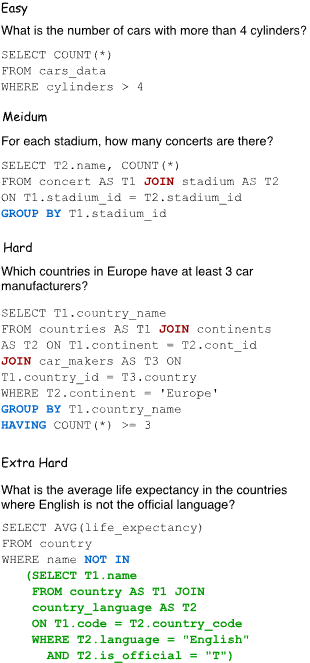
\includegraphics[width=0.35\textwidth]{image.png}
\caption{SQL query examples in 4 hardness levels. Credit: Spider [1]}
\label{fig:hardness-levels}
\end{figure}

\subsection{Prompting and Input}
\label{sec:prompting}

Each model receives three pieces of information in a single zero-shot user turn: a system instruction explaining its role as a Text-to-SQL generator, the database schema (table names, column names, primary keys, and foreign-key relationships, with no example rows), and the natural-language question. No few-shot examples are provided, so that the experiment measures each model's ability to generate SQL from instructions and schema information alone, without the confound of examples steering its output style. The prompt template is identical across all three models, so that differences in performance can be attributed to the models rather than to differences in prompting.

\textbf{Prompt template:}
\begin{verbatim}
Given the following SQLite database schema, write a SQL query that answers
the question.

{schema}

Question: {question}

Respond with only the SQL query in a ```sql code block.
\end{verbatim}

See \hyperref[sec:appendix1]{Appendix 1} for a worked example: a full schema, a question, and the resulting filled prompt.

\subsection{SQL Extraction}
\label{sec:sql-extraction}

For each sample, we decode the model's generated tokens into text using the model-specific tokenizer, and check for the presence of a \texttt{</think>} token. If \texttt{</think>} was generated, we take all text generated before \texttt{</think>} as the reasoning trace and all text to the right as the output SQL; DeepSeek-R1-Distill-Qwen-1.5B is the only model of the three that can emit this token. The SQL is then extracted from the first \texttt{```sql} code block in that remaining text. The extracted SQL is passed to the evaluation script as-is. Outputs that cannot be extracted or parsed are counted as incorrect on every metric rather than excluded from the evaluation, as unusable output is a task failure (see \ref{sec:evaluation-metrics} and \ref{sec:invalid-outputs}).

\subsection{Inference Settings}
\label{sec:inference-settings}

All models are evaluated using the same decoding configuration: greedy decoding (temperature and top-p are not applicable) for consistent, reproducible results between runs. The maximum output length differs by model: 256 tokens for Qwen3-0.6B, and 4096 tokens for both Qwen3-4B and DeepSeek-R1-Distill-Qwen-1.5B. For DeepSeek, the larger budget is needed because its output also has to contain a full reasoning trace rather than only the SQL query; Qwen3-4B is given the same, larger budget as DeepSeek so that a tighter token limit can be ruled out as the reason for any difference between them on invalid-output rate (\ref{sec:invalid-outputs}) or inference time (\ref{sec:efficiency}). Qwen3-0.6B and Qwen3-4B are both run with thinking mode off (both support it). DeepSeek-R1-Distill-Qwen-1.5B always produces a reasoning trace and has no documented way to disable thinking mode, so it is evaluated as the reasoning condition against the two non-reasoning Qwen3 models. All inference runs on the same 1x RTX 4090 GPU described in \ref{sec:models}, with batch size 1.

\subsection{Evaluation}
\label{sec:evaluation-metrics}

We evaluate the output using the same metrics as the Spider paper [1]. These are:

\begin{enumerate}
\item Component Matching
    \begin{itemize}
        \item For each of the following components:
        \begin{itemize}
            \item SELECT
            \item WHERE
            \item GROUP BY
            \item ORDER BY
            \item KEYWORDS (including all SQL keywords without column names and operators)
        \end{itemize}
        \item Decompose each component in the prediction and ground truth as bags of several sub-components and check whether or not these two sets of components match completely.
        \item Checks accuracy, recall, and F1
    \end{itemize}
\item Exact Matching Accuracy
    \begin{itemize}
        \item We measure whether the generated query as a whole is equivalent to the last section
        \item The generated query is correct only if all components are correct
        \item Checks only accuracy
    \end{itemize}
\item Execution Accuracy
    \begin{itemize}
        \item A list of gold values for each question is given
        \item We measure how many gold values the generated query extracts when executed
        \item Checks only accuracy
    \end{itemize}
\end{enumerate}

If output is invalid or unparsable, then it fails all 3 dimensions (component matching, exact matching, execution accuracy), consistent with how \ref{sec:sql-extraction} extracts and passes SQL to this evaluation script. This is reasonable as invalid/unparsable output cannot be applied to SQL and thus must be avoided and penalized heavily; Results~\ref{sec:invalid-outputs} reports how often this happens for each model.

\section{Task 1 -- RQ1: Results}
\label{sec:rq1-results}

\subsection{Overall Model Performance}
\label{sec:overall-performance}

Below we report how Qwen3-0.6B, Qwen3-4B, and Deepseek-R1-Distill-Qwen3-1.5B perform on the Spider benchmark across all 3 metrics (Component Matching, Exact Matching Accuracy, Execution Accuracy). We calculate the values per problem difficulty as well as overall, and display them in the below tables.

\begin{table}[H]
\centering
\footnotesize
\caption{Overall performance summary, aggregated across all difficulties (all 1034 problems). Component matching is accuracy / recall / F1 (macro-averaged, see the note on table~\ref{tab:difficulty-component} in \ref{sec:rq1-interpretation}). Per-difficulty breakdowns are in tables~\ref{tab:difficulty-component}--\ref{tab:difficulty-execution}.}
\label{tab:overall-performance}
\resizebox{\textwidth}{!}{%
\begin{tabular}{lllccc}
\toprule
Model & Parameters & Category & Component matching & Exact matching & Execution accuracy \\
\midrule
Qwen3-0.6B & 0.6B & Decoder-only & 0.628 / 0.209 / 0.314 & 0.099 & 0.209 \\
Qwen3-4B & 4B & Decoder-only & 0.797 / 0.306 / 0.442 & 0.256 & 0.353 \\
DeepSeek-R1-Distill-Qwen-1.5B & 1.5B & Reasoning & 0.661 / 0.174 / 0.275 & 0.085 & 0.121 \\
\bottomrule
\end{tabular}}
\end{table}

All models are evaluated zero-shot with the same prompt on the 20 databases of the Spider dev set. Aggregated across all difficulties and databases, every model is still far from solving the task: execution accuracy ranges from 0.121 (DeepSeek) to 0.353 (Qwen3-4B) and exact matching accuracy from 0.085 (DeepSeek) to 0.256 (Qwen3-4B). Execution accuracy is higher than exact matching accuracy for all three models (for example 0.353 vs.\ 0.256 for Qwen3-4B), which suggests that at least some of the queries that return the correct result are written differently from the gold SQL (see \ref{sec:rq1-interpretation} for more on this relationship). Of the three models, Qwen3-4B is now the best on almost every metric, database, and difficulty level; \ref{sec:by-database} and \ref{sec:rq1-interpretation} quantify how consistently. Table~\ref{tab:inference-time} reports the efficiency side of this comparison: inference time per example.

\subsection{Performance by Query Difficulty}
\label{sec:by-difficulty}

\begin{table}[H]
\centering
\footnotesize
\caption{Component matching (accuracy / recall / F1) by difficulty.}
\label{tab:difficulty-component}
\begin{tabular}{lcc}
\toprule
Model & easy & medium \\
\midrule
Problems (n) & 248 & 446 \\
Qwen3-0.6B & 0.675 / 0.308 / 0.423 & 0.582 / 0.235 / 0.334 \\
Qwen3-4B & 0.838 / 0.574 / 0.681 & 0.670 / 0.306 / 0.420 \\
DeepSeek-R1-Distill-Qwen-1.5B & 0.566 / 0.288 / 0.382 & 0.642 / 0.185 / 0.287 \\
\bottomrule
\end{tabular}

\vspace{0.5em}

\begin{tabular}{lccc}
\toprule
Model & hard & extra & all \\
\midrule
Problems (n) & 174 & 166 & 1034 \\
Qwen3-0.6B & 0.540 / 0.141 / 0.223 & 0.578 / 0.160 / 0.250 & 0.628 / 0.209 / 0.314 \\
Qwen3-4B & 0.796 / 0.262 / 0.394 & 0.485 / 0.150 / 0.229 & 0.797 / 0.306 / 0.442 \\
DeepSeek-R1-Distill-Qwen-1.5B & 0.543 / 0.113 / 0.187 & 0.389 / 0.104 / 0.164 & 0.661 / 0.174 / 0.275 \\
\bottomrule
\end{tabular}
\end{table}

\begin{table}[H]
\centering
\footnotesize
\caption{Exact matching accuracy by difficulty.}
\label{tab:difficulty-exact}
\begin{tabular}{lccccc}
\toprule
Model & easy & medium & hard & extra & all \\
\midrule
Problems (n) & 248 & 446 & 174 & 166 & 1034 \\
Qwen3-0.6B & 0.157 & 0.137 & 0.006 & 0.006 & 0.099 \\
Qwen3-4B & 0.508 & 0.262 & 0.115 & 0.012 & 0.256 \\
DeepSeek-R1-Distill-Qwen-1.5B & 0.214 & 0.078 & 0.000 & 0.000 & 0.085 \\
\bottomrule
\end{tabular}
\end{table}

\begin{table}[H]
\centering
\footnotesize
\caption{Execution accuracy by difficulty.}
\label{tab:difficulty-execution}
\begin{tabular}{lccccc}
\toprule
Model & easy & medium & hard & extra & all \\
\midrule
Problems (n) & 248 & 446 & 174 & 166 & 1034 \\
Qwen3-0.6B & 0.210 & 0.276 & 0.126 & 0.114 & 0.209 \\
Qwen3-4B & 0.565 & 0.345 & 0.276 & 0.139 & 0.353 \\
DeepSeek-R1-Distill-Qwen-1.5B & 0.258 & 0.128 & 0.017 & 0.006 & 0.121 \\
\bottomrule
\end{tabular}
\end{table}

We break every metric down by the Spider Hardness Criteria (\ref{sec:eval-data}) as query difficulty is a first-order driver of Text-to-SQL performance; comparing models only in aggregate would hide whether a model's advantage holds up as queries get harder.

Performance decreases with difficulty for every model, but the decrease is steepest for Qwen3-0.6B and DeepSeek: their exact matching and execution accuracy are both at most 0.034 and 0.126 respectively on hard and extra problems, down from as high as 0.210-0.258 (easy execution) on the easiest problems (table~\ref{tab:difficulty-exact} and table~\ref{tab:difficulty-execution}). Qwen3-4B degrades on the same relative scale but from a much higher starting point, from 0.508 easy exact matching / 0.565 easy execution accuracy down to 0.012 extra exact matching / 0.139 extra execution accuracy. Despite the degredation, it remains the best of the three models at every single difficulty level on both metrics (tables~\ref{tab:difficulty-exact}--\ref{tab:difficulty-execution}).

\subsection{Performance by Database}
\label{sec:by-database}

We also break execution and exact matching accuracy down by each of the 20 Spider dev databases. Qwen3-4B has the highest execution accuracy on 17 of the 20 databases outright (plus a tie on one more) and the highest exact matching accuracy on 18 of 20, while DeepSeek-R1-Distill-Qwen-1.5B is never highest on either metric; Qwen3-0.6B wins outright only on orchestra and battle\_death. Databases with few problems (real\_estate\_properties with n=4, voter\_1 with n=15, battle\_death with n=16, and museum\_visit with n=18) are too small to rank the models reliably, since a single problem changes a score by 6 to 25 percentage points. Execution accuracy ranges from 0.10 (course\_teach) to 0.53 (singer) for Qwen3-0.6B, from 0.19 (battle\_death) to 0.60 (singer) for Qwen3-4B, and from 0.00 (concert\_singer) to 0.27 (singer and voter\_1) for DeepSeek-R1-Distill-Qwen-1.5B (\hyperref[tab:db-execution]{Table 5}). The pattern on exact matching accuracy is just as one-sided (\hyperref[tab:db-exact]{Table 6}): Qwen3-4B is highest on 18 of 20 databases, ties Qwen3-0.6B on orchestra, and loses only on battle\_death; DeepSeek's exact matching accuracy is never the highest of the three, coming closest on flight\_2 (0.200 vs.\ Qwen3-4B's 0.350 and Qwen3-0.6B's 0.075). The full per-database tables and discussion are in \hyperref[sec:appendix2]{Appendix 2}.

\subsection{Invalid and Unparseable Outputs}
\label{sec:invalid-outputs}

We also count how often each model's output cannot be used as SQL at all: it either never produces a usable query within the token budget (\ref{sec:inference-settings}) or is truncated before finishing one. Per \ref{sec:evaluation-metrics}, these count as failures on every metric rather than being excluded, and this is a direct measure of how reliably each model follows the ``respond with only a SQL query'' instruction, independent of whether the SQL it does produce is correct. Qwen3-0.6B's invalid rate is 2.2\%, Qwen3-4B's is 0.0\%, and DeepSeek-R1-Distill-Qwen-1.5B's is 9.7\%, about 4x higher than Qwen3-0.6B's despite having the same 4096-token budget as Qwen3-4B (\ref{sec:inference-settings}), i.e. a larger token budget did not cause Qwen3-4B to run on or produce unusable output the way it does for DeepSeek. \ref{sec:rq1-interpretation} breaks DeepSeek's failures down further by difficulty and by why the generation failed (tables~\ref{tab:deepseek-outcome}--\ref{tab:deepseek-unfinished-by-difficulty}).

\subsection{Efficiency Measures}
\label{sec:efficiency}

\begin{table}[H]
\centering
\footnotesize
\caption{Output tokens per example}
\label{tab:tokens-per-example}
\begin{tabular}{lccccc}
\toprule
Model & easy & medium & hard & extra & all \\
\midrule
Qwen3-0.6B & 27.5 & 44.7 & 53.7 & 69.9 & 46.1 \\
Qwen3-4B & 23.6 & 37.3 & 46.2 & 59.0 & 39.0 \\
DeepSeek-R1-Distill-Qwen-1.5B & 610.8 & 768.4 & 1096.0 & 1176.9 & 851.3 \\
\bottomrule
\end{tabular}
\end{table}

Inference time is measured from the start of generation to the complete batch output, per batch of 1 example, excluding tokenization, model loading, and warm-up.

\begin{table}[H]
\centering
\footnotesize
\caption{Inference time.}
\label{tab:inference-time}
\begin{tabular}{lcc}
\toprule
Model & Total wall time (s) & Avg.\ time per example (s) \\
\midrule
Qwen3-0.6B & 123.9 & 0.120 \\
Qwen3-4B & 109.1 & 0.106 \\
DeepSeek-R1-Distill-Qwen-1.5B & 3059.8 & 2.959 \\
\bottomrule
\end{tabular}
\end{table}

DeepSeek is about 25x slower per example than Qwen3-0.6B and 28x slower than Qwen3-4B, consistent with its much higher average token count (table~\ref{tab:tokens-per-example}). Qwen3-4B, despite having about 7x as many parameters as Qwen3-0.6B, is marginally faster per example (0.106s vs.\ 0.120s), consistent with it generating fewer tokens on average (39.0 vs.\ 46.1, table~\ref{tab:tokens-per-example}) despite having the same 16x larger token budget as DeepSeek (\ref{sec:inference-settings}).

\begin{table}[H]
\centering
\footnotesize
\caption{DeepSeek-R1-Distill-Qwen-1.5B by generation outcome. ``Cut'' means the generation reached the 4096-token limit.}
\label{tab:deepseek-outcome}
\begin{tabular}{lccccc}
\toprule
Outcome & Problems (n) & Share & Avg.\ tokens & Exact match & Component F1 \\
\midrule
Finished with SQL & 934 & 90.3\% & 512 & 0.094 & 0.286 \\
Finished, no usable SQL & 2 & 0.2\% & 284 & 0.000 & 0.100 \\
Cut while answering (after \texttt{</think>}) & 13 & 1.3\% & 4096 & 0.000 & 0.096 \\
Cut while thinking (no \texttt{</think>}) & 85 & 8.2\% & 4096 & 0.000 & 0.093 \\
All & 1034 & 100\% & 851 & 0.085 & 0.275 \\
\bottomrule
\end{tabular}
\end{table}

\begin{table}[H]
\centering
\footnotesize
\caption{The same 934 questions that DeepSeek finished, for all three models.}
\label{tab:deepseek-finished-934}
\begin{tabular}{lcc}
\toprule
Model & Exact match & Component F1 \\
\midrule
DeepSeek-R1-Distill-Qwen-1.5B & 0.094 & 0.286 \\
Qwen3-0.6B & 0.103 & 0.317 \\
Qwen3-4B & 0.257 & 0.440 \\
\bottomrule
\end{tabular}
\end{table}

\begin{table}[H]
\centering
\footnotesize
\caption{Are the cut-off DeepSeek generations infinite self-repetition loops? A text that repeats itself compresses well, so a low compression ratio of the last 3000 characters indicates a loop.}
\label{tab:deepseek-repetition}
\begin{tabular}{lcccc}
\toprule
Generations & n & Median compression ratio & Ratio $<$ 0.15 & Last 150 characters repeat 3 or more times \\
\midrule
Cut off & 98 & 0.095 & 95.9\% & 96.9\% \\
Finished & 936 & 0.418 & 0.0\% & 0.2\% \\
\bottomrule
\end{tabular}
\end{table}

\begin{table}[H]
\centering
\footnotesize
\caption{Share of DeepSeek generations that did not finish with SQL, by difficulty.}
\label{tab:deepseek-unfinished-by-difficulty}
\begin{tabular}{lccccc}
\toprule
 & easy & medium & hard & extra & all \\
\midrule
Problems (n) & 248 & 446 & 174 & 166 & 1034 \\
Not finished with SQL (n) & 15 & 33 & 25 & 27 & 100 \\
Share & 6.0\% & 7.4\% & 14.4\% & 16.3\% & 9.7\% \\
\bottomrule
\end{tabular}
\end{table}

\section{Interpretation and Answer to Research Question (RQ1)}
\label{sec:rq1-interpretation}

\textbf{RQ1:} How do (selected) LLMs perform on cross-domain Text-to-SQL?

\vspace{10px}

All three models are still far from solving the task in this zero-shot setting: exact matching accuracy ranges from 0.085 to 0.256 and execution accuracy from 0.121 to 0.353 (table~\ref{tab:overall-performance}). Difficulty and database effects are discussed in \ref{sec:by-difficulty} and \ref{sec:by-database}; here we interpret the effects of model size and reasoning architecture and the exact-match/execution-accuracy relationship, and state the answer to RQ1 as three findings.

\textbf{First, within the Qwen family, scale is a strong and almost uniform predictor of performance, but an intermediate-size reasoning model from the Deepseek family still loses to the smallest model in the Qwen family.} Aggregated across all difficulties, Qwen3-4B has the best component matching (0.797 / 0.306 / 0.442), exact matching (0.256), and execution accuracy (0.353) of the three (table~\ref{tab:overall-performance}), and it beats Qwen3-0.6B on exact matching and execution accuracy at every individual difficulty level, including hard (0.115 vs.\ 0.006) and extra (0.012 vs.\ 0.006), where the smaller model solves almost nothing (tables~\ref{tab:difficulty-exact}--\ref{tab:difficulty-execution}). This is the largest, most consistent effect in the RQ1 results. The one exception is component matching on extra-hard problems, where Qwen3-0.6B's accuracy, recall, and F1 (0.578 / 0.160 / 0.250) are all slightly higher than Qwen3-4B's (0.485 / 0.150 / 0.229), the only point in the RQ1 results where the smaller Qwen3 model wins outright (table~\ref{tab:difficulty-component}). DeepSeek-R1-Distill-Qwen-1.5B sits between the two Qwen3 models in parameter count (1.5B) and is the only one that reasons, yet it is the lowest of the three on every aggregate metric (0.275 component F1, 0.085 exact matching, 0.121 execution accuracy) except its own component-matching accuracy (0.661 vs.\ 0.628 for Qwen3-0.6B). Thus, scale predicts performance well within a family, but does not transfer across the reasoning/non-reasoning boundary: having more parameters than Qwen3-0.6B did not help DeepSeek catch up to it.

\textbf{Second, the reasoning architecture itself, not parameter count, is the main driver of DeepSeek's low score.} Its invalid-output rate (9.7\%) is markedly higher than Qwen3-0.6B's (2.2\%) and Qwen3-4B's (0.0\% in this run) (\ref{sec:invalid-outputs}). In tables~\ref{tab:deepseek-outcome}--\ref{tab:deepseek-unfinished-by-difficulty}, 100 of 1034 generations (9.7\%) end without usable SQL. 85 never leave the reasoning phase, 13 are cut while writing the answer, and 2 finish without SQL. The number of unusable SQL generations also grows with difficulty, from 6.0\% on easy to 16.3\% on extra problems. These are not cases of long productive reasoning either: 95.9\% of the cut-off generations are highly self-repetitive (compression ratio below 0.15, median compression ratio 0.095, vs.\ 0.418 for finished generations), rewriting the same query and repeating phrases like ``So the final query is:'' without converging. Finishing does not make it better either: on the 934 questions DeepSeek does finish, its exact matching (0.094) and component F1 (0.286) are still below Qwen3-0.6B's on the same questions (0.103 / 0.317) and far below Qwen3-4B's (0.257 / 0.440), despite generating 512 tokens per question on average there, against 46 and 39 tokens overall for Qwen3-0.6B and Qwen3-4B (about 18x and 22x fewer). This extra length also costs time: DeepSeek is 25-28x slower per example than either Qwen3 model (\ref{sec:efficiency}). The reasoning trace mostly lengthens the output and sometimes never terminates, without improving the SQL when it does, and size alone is not the explanation, since Qwen3-4B is both bigger than DeepSeek and the best model in the comparison. Thus, reasoning architecture itself, not the parameter count, is the main driver of DeepSeek's low score.

\textbf{Third, query difficulty has a substantial, consistent effect on every model, including the best one.} Exact matching and execution accuracy both fall sharply from easy to extra-hard problems for all three models (\ref{sec:by-difficulty}). Qwen3-4B's drop is from a much higher base (0.508 to 0.012 exact matching, 0.565 to 0.139 execution accuracy) and it remains the best model at every difficulty level on both metrics, but the drop itself is just as steep in relative terms as for the other two models, and the hardest problems remain largely unsolved even for it.

\textbf{Exact match vs.\ execution accuracy.} For all three models, execution accuracy aggregated across all difficulties exceeds exact matching accuracy (table~\ref{tab:overall-performance}): 0.209 vs.\ 0.099 for Qwen3-0.6B, 0.353 vs.\ 0.256 for Qwen3-4B, and 0.121 vs.\ 0.085 for DeepSeek. Since exact matching requires every SQL component to match the gold query while execution accuracy only requires the same result set, this gap indicates each model writes some queries that are valid and correct but phrased differently from the gold SQL (e.g.\ a different but equivalent join order, or an explicit column list where the gold query uses \texttt{SELECT *}). The gap is widest for Qwen3-0.6B (11.0 points), close behind for Qwen3-4B (9.7 points), and narrowest for DeepSeek (3.6 points); DeepSeek's narrower gap reflects it producing fewer alternative-but-valid queries. Qwen3-4B's gap is almost as wide as Qwen3-0.6B's despite much higher absolute accuracy, so scaling up within the Qwen3 family raises both Exact Match Accuracy and Execution Accuracy together rather than closing the gap between them.

\textbf{Limitations.} Our working hypothesis is that Text-to-SQL at this scale does not benefit from an explicit reasoning trace, and that a non-reasoning model is sufficient, with performance instead scaling with parameter count within a fixed model family. The results are consistent with this hypothesis. However, they do not establish that Text-to-SQL is too simple for reasoning models in general due to several factors:

\begin{itemize}
\item \textbf{Truncation and failed outputs for DeepSeek.} These count as failures on every metric and lower its recall, exact matching, and execution scores, but table~\ref{tab:deepseek-finished-934} shows removing them would not change the ranking (DeepSeek is also lower on the questions it finished), and table~\ref{tab:deepseek-repetition} shows the cut-off generations are repetition loops, so a larger token budget is unlikely to rescue them.
\item \textbf{Model differences beyond reasoning.} Qwen3-0.6B and Qwen3-4B share a model family, isolating the effect of scale between them, but DeepSeek differs from both in family, size, and pretraining/post-training, not only in whether it reasons; it is also a distilled model, so the effect of reasoning cannot be fully separated from distillation quality.
\item \textbf{Aggregated component matching.} The component matching figures in table~\ref{tab:difficulty-component} (and in table~\ref{tab:overall-performance}) are our own macro-average (mean of the 10 per-component accuracy and recall scores, with F1 computed from these two means), not a number reported by Spider.
\end{itemize}

Overall, in this zero-shot, cross-domain setting, a larger non-reasoning decoder-only model (Qwen3-4B, 4B) clearly outperforms both a same-family model at under a sixth its size (Qwen3-0.6B) and a reasoning model of intermediate size from a different family (DeepSeek-R1-Distill-Qwen-1.5B, 1.5B), while also being faster per example than either. None of the three models solve more than half of even the easiest problems or more than a small fraction of hard or extra-hard queries. This answers RQ1 for the three models evaluated.
 into REPORT.tex in place of the current inline
% "Task 1 -- RQ1: Methodology & Results" / "Task 1 -- RQ1: Results" content.
% REPORT.tex already loads every package this fragment needs (booktabs, array,
% graphicx, float, caption, hyperref), so no extra preamble is required.
%
% Annotations made while converting this to reference-based numbering:
%  - All \subsection*{N.M ...} / \section*{...} became real, numbered
%    \section/\subsection commands with the leading "N.M" stripped from the
%    title text (LaTeX now generates it), each with a \label. The former
%    \subsection*{3. Interpretation...} is promoted to a top-level \section,
%    since it was already numbered as a peer of Parts 1 and 2, not a child
%    of Part 2.
%  - Every table/figure got a \label right after its \caption, and every
%    in-text "table 1", "tables 2-4", "2.2", "Appendix 2", etc. became a
%    \ref (or \hyperref for Appendix 2/3, which live outside this file --
%    see note below). Because the Models table (1.1) is now counted and the
%    Appendix 2/3 tables are not part of this file's sequential numbering,
%    the printed table numbers shift versus the pasted draft (e.g. "table 1"
%    -> Table 2, "table 8" -> Table 6); every mention uses \ref, so this is
%    self-consistent and will stay correct if tables move again.
%  - Fixed a leftover inconsistency in 1.5: the draft's 1.1 and 2.5 both
%    state batch size 1 (confirmed correct), but 1.5 still said "batch size
%    128" (leftover from an earlier draft) -- corrected to 1.
%  - Both TODOs in the pasted draft are resolved inline: 2.2 now cites
%    Tables 4-5 directly instead of a placeholder, and 2.3 now cites the
%    concrete per-database numbers from Appendix 2 (pulled from REPORT.tex's
%    existing Appendix 2 prose) instead of a placeholder.
%  - The Overall Performance table's caption promises "the note on table 2
%    in 3" (i.e. a note about macro-averaged component matching, to appear
%    in the Interpretation section), but the pasted draft's Limitations list
%    dropped that bullet (it only kept "Truncation" and "Model differences").
%    Restored the "Aggregated component matching" bullet from the prior
%    REPORT.tex draft so the caption's forward reference resolves to real
%    content; this is a content restoration, not just a labeling change,
%    so flagging it here. The other previously-present bullet ("Single run
%    and sample size") was NOT restored, since nothing in the new draft
%    points to it -- worth confirming with the author whether that drop was
%    intentional.
%  - Appendix 1/2/3 and their tables (5, 6, 7) live in REPORT.tex, outside
%    this file. REPORT.tex's appendix tables keep their existing manual
%    "Table 5/6/7:" caption numbering (renumbering them would require
%    restructuring the whole document's table order, which is out of scope
%    here); \label{tab:db-execution}, \label{tab:db-exact} and
%    \label{tab:invalid-outputs} were added to those tables in REPORT.tex
%    (additive only, no visible change) so this file can link to them.
%    Since their printed numbers are not auto-generated, this file links to
%    them with \hyperref[label]{5}-style calls (a real clickable link, with
%    text matching the manual number already in their caption) rather than
%    \ref (which would print whatever their true document-order table
%    number is, not 5/6/7).

\section{Task 1 -- RQ1: Methodology \& Results}
\label{sec:rq1-methods}

\textbf{RQ1:} How do (selected) LLMs perform on cross-domain Text-to-SQL?

In this report we evaluate the performance of decoder-only language models as well as reasoning LLMs on cross-domain SQL.

\subsection{Models}
\label{sec:models}

We compare two decoder-only LLMs from the same model family at different scales (Qwen3-0.6B and Qwen3-4B) against one reasoning LLM, so that the comparison isolates the effect of scale within a fixed family from the effect of an explicit reasoning trace, as much as a 3-model study can. All three are accessed as local inference over their bf16 Huggingface checkpoints on 1x NVIDIA GeForce RTX 4090 GPU (no API-based models), so that inference parameters are fully under our control (see \ref{sec:inference-settings}). We evaluate using batch sizes of 1.

\begin{table}[H]
\centering
\footnotesize
\caption{Models compared in RQ1.}
\label{tab:models}
\resizebox{\textwidth}{!}{%
\begin{tabular}{llllll}
\toprule
Model & Category & Parameters & Quantization & Access & Thinking mode \\
\midrule
Qwen3-0.6B [2] & Decoder-only & 0.6B & bf16 (none beyond release precision) & Local, Huggingface checkpoint & Disabled \\
Qwen3-4B [2] & Decoder-only & 4B & bf16 (none beyond release precision) & Local, Huggingface checkpoint & Disabled \\
DeepSeek-R1-Distill-Qwen-1.5B [4] & Reasoning & 1.5B & bf16 (none beyond release precision) & Local, Huggingface checkpoint & Always on (no disable option) \\
\bottomrule
\end{tabular}}
\end{table}

All three are dense (non-MoE) models, so no distinction between total and active parameters applies.

\subsection{Evaluation Data}
\label{sec:eval-data}

We use all 1034 examples in the Spider [1] development split, with no subsampling and therefore no sampling seed to report; every example is included, so the per-database counts below and the per-database results tables (\hyperref[tab:db-execution]{5} and \hyperref[tab:db-exact]{6}) enumerate exactly which examples are used. To evaluate cross-domain performance, we additionally report results separately for each of the 20 databases in the Spider dev set: world\_1 (120 problems), car\_1 (92), cre\_Doc\_Template\_Mgt (84), dog\_kennels (82), flight\_2 (80), student\_transcripts\_tracking (78), wta\_1 (62), tvshow (62), network\_1 (56), concert\_singer (45), pets\_1 (42), poker\_player (40), orchestra (40), employee\_hire\_evaluation (38), course\_teach (30), singer (30), museum\_visit (18), battle\_death (16), voter\_1 (15), and real\_estate\_properties (4).

We also use the Spider Hardness Criteria, where queries are assigned difficulties based on the number of SQL components, selections, and conditions, so that queries that contain more SQL keywords are considered harder.

\begin{figure}[H]
\centering
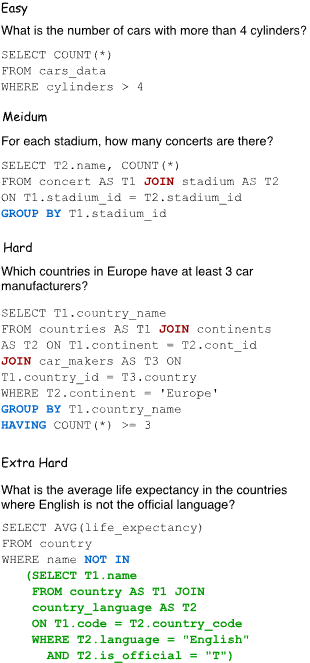
\includegraphics[width=0.35\textwidth]{image.png}
\caption{SQL query examples in 4 hardness levels. Credit: Spider [1]}
\label{fig:hardness-levels}
\end{figure}

\subsection{Prompting and Input}
\label{sec:prompting}

Each model receives three pieces of information in a single zero-shot user turn: a system instruction explaining its role as a Text-to-SQL generator, the database schema (table names, column names, primary keys, and foreign-key relationships, with no example rows), and the natural-language question. No few-shot examples are provided, so that the experiment measures each model's ability to generate SQL from instructions and schema information alone, without the confound of examples steering its output style. The prompt template is identical across all three models, so that differences in performance can be attributed to the models rather than to differences in prompting.

\textbf{Prompt template:}
\begin{verbatim}
Given the following SQLite database schema, write a SQL query that answers
the question.

{schema}

Question: {question}

Respond with only the SQL query in a ```sql code block.
\end{verbatim}

See \hyperref[sec:appendix1]{Appendix 1} for a worked example: a full schema, a question, and the resulting filled prompt.

\subsection{SQL Extraction}
\label{sec:sql-extraction}

For each sample, we decode the model's generated tokens into text using the model-specific tokenizer, and check for the presence of a \texttt{</think>} token. If \texttt{</think>} was generated, we take all text generated before \texttt{</think>} as the reasoning trace and all text to the right as the output SQL; DeepSeek-R1-Distill-Qwen-1.5B is the only model of the three that can emit this token. The SQL is then extracted from the first \texttt{```sql} code block in that remaining text. The extracted SQL is passed to the evaluation script as-is. Outputs that cannot be extracted or parsed are counted as incorrect on every metric rather than excluded from the evaluation, as unusable output is a task failure (see \ref{sec:evaluation-metrics} and \ref{sec:invalid-outputs}).

\subsection{Inference Settings}
\label{sec:inference-settings}

All models are evaluated using the same decoding configuration: greedy decoding (temperature and top-p are not applicable) for consistent, reproducible results between runs. The maximum output length differs by model: 256 tokens for Qwen3-0.6B, and 4096 tokens for both Qwen3-4B and DeepSeek-R1-Distill-Qwen-1.5B. For DeepSeek, the larger budget is needed because its output also has to contain a full reasoning trace rather than only the SQL query; Qwen3-4B is given the same, larger budget as DeepSeek so that a tighter token limit can be ruled out as the reason for any difference between them on invalid-output rate (\ref{sec:invalid-outputs}) or inference time (\ref{sec:efficiency}). Qwen3-0.6B and Qwen3-4B are both run with thinking mode off (both support it). DeepSeek-R1-Distill-Qwen-1.5B always produces a reasoning trace and has no documented way to disable thinking mode, so it is evaluated as the reasoning condition against the two non-reasoning Qwen3 models. All inference runs on the same 1x RTX 4090 GPU described in \ref{sec:models}, with batch size 1.

\subsection{Evaluation}
\label{sec:evaluation-metrics}

We evaluate the output using the same metrics as the Spider paper [1]. These are:

\begin{enumerate}
\item Component Matching
    \begin{itemize}
        \item For each of the following components:
        \begin{itemize}
            \item SELECT
            \item WHERE
            \item GROUP BY
            \item ORDER BY
            \item KEYWORDS (including all SQL keywords without column names and operators)
        \end{itemize}
        \item Decompose each component in the prediction and ground truth as bags of several sub-components and check whether or not these two sets of components match completely.
        \item Checks accuracy, recall, and F1
    \end{itemize}
\item Exact Matching Accuracy
    \begin{itemize}
        \item We measure whether the generated query as a whole is equivalent to the last section
        \item The generated query is correct only if all components are correct
        \item Checks only accuracy
    \end{itemize}
\item Execution Accuracy
    \begin{itemize}
        \item A list of gold values for each question is given
        \item We measure how many gold values the generated query extracts when executed
        \item Checks only accuracy
    \end{itemize}
\end{enumerate}

If output is invalid or unparsable, then it fails all 3 dimensions (component matching, exact matching, execution accuracy), consistent with how \ref{sec:sql-extraction} extracts and passes SQL to this evaluation script. This is reasonable as invalid/unparsable output cannot be applied to SQL and thus must be avoided and penalized heavily; Results~\ref{sec:invalid-outputs} reports how often this happens for each model.

\section{Task 1 -- RQ1: Results}
\label{sec:rq1-results}

\subsection{Overall Model Performance}
\label{sec:overall-performance}

Below we report how Qwen3-0.6B, Qwen3-4B, and Deepseek-R1-Distill-Qwen3-1.5B perform on the Spider benchmark across all 3 metrics (Component Matching, Exact Matching Accuracy, Execution Accuracy). We calculate the values per problem difficulty as well as overall, and display them in the below tables.

\begin{table}[H]
\centering
\footnotesize
\caption{Overall performance summary, aggregated across all difficulties (all 1034 problems). Component matching is accuracy / recall / F1 (macro-averaged, see the note on table~\ref{tab:difficulty-component} in \ref{sec:rq1-interpretation}). Per-difficulty breakdowns are in tables~\ref{tab:difficulty-component}--\ref{tab:difficulty-execution}.}
\label{tab:overall-performance}
\resizebox{\textwidth}{!}{%
\begin{tabular}{lllccc}
\toprule
Model & Parameters & Category & Component matching & Exact matching & Execution accuracy \\
\midrule
Qwen3-0.6B & 0.6B & Decoder-only & 0.628 / 0.209 / 0.314 & 0.099 & 0.209 \\
Qwen3-4B & 4B & Decoder-only & 0.797 / 0.306 / 0.442 & 0.256 & 0.353 \\
DeepSeek-R1-Distill-Qwen-1.5B & 1.5B & Reasoning & 0.661 / 0.174 / 0.275 & 0.085 & 0.121 \\
\bottomrule
\end{tabular}}
\end{table}

All models are evaluated zero-shot with the same prompt on the 20 databases of the Spider dev set. Aggregated across all difficulties and databases, every model is still far from solving the task: execution accuracy ranges from 0.121 (DeepSeek) to 0.353 (Qwen3-4B) and exact matching accuracy from 0.085 (DeepSeek) to 0.256 (Qwen3-4B). Execution accuracy is higher than exact matching accuracy for all three models (for example 0.353 vs.\ 0.256 for Qwen3-4B), which suggests that at least some of the queries that return the correct result are written differently from the gold SQL (see \ref{sec:rq1-interpretation} for more on this relationship). Of the three models, Qwen3-4B is now the best on almost every metric, database, and difficulty level; \ref{sec:by-database} and \ref{sec:rq1-interpretation} quantify how consistently. Table~\ref{tab:inference-time} reports the efficiency side of this comparison: inference time per example.

\subsection{Performance by Query Difficulty}
\label{sec:by-difficulty}

\begin{table}[H]
\centering
\footnotesize
\caption{Component matching (accuracy / recall / F1) by difficulty.}
\label{tab:difficulty-component}
\begin{tabular}{lcc}
\toprule
Model & easy & medium \\
\midrule
Problems (n) & 248 & 446 \\
Qwen3-0.6B & 0.675 / 0.308 / 0.423 & 0.582 / 0.235 / 0.334 \\
Qwen3-4B & 0.838 / 0.574 / 0.681 & 0.670 / 0.306 / 0.420 \\
DeepSeek-R1-Distill-Qwen-1.5B & 0.566 / 0.288 / 0.382 & 0.642 / 0.185 / 0.287 \\
\bottomrule
\end{tabular}

\vspace{0.5em}

\begin{tabular}{lccc}
\toprule
Model & hard & extra & all \\
\midrule
Problems (n) & 174 & 166 & 1034 \\
Qwen3-0.6B & 0.540 / 0.141 / 0.223 & 0.578 / 0.160 / 0.250 & 0.628 / 0.209 / 0.314 \\
Qwen3-4B & 0.796 / 0.262 / 0.394 & 0.485 / 0.150 / 0.229 & 0.797 / 0.306 / 0.442 \\
DeepSeek-R1-Distill-Qwen-1.5B & 0.543 / 0.113 / 0.187 & 0.389 / 0.104 / 0.164 & 0.661 / 0.174 / 0.275 \\
\bottomrule
\end{tabular}
\end{table}

\begin{table}[H]
\centering
\footnotesize
\caption{Exact matching accuracy by difficulty.}
\label{tab:difficulty-exact}
\begin{tabular}{lccccc}
\toprule
Model & easy & medium & hard & extra & all \\
\midrule
Problems (n) & 248 & 446 & 174 & 166 & 1034 \\
Qwen3-0.6B & 0.157 & 0.137 & 0.006 & 0.006 & 0.099 \\
Qwen3-4B & 0.508 & 0.262 & 0.115 & 0.012 & 0.256 \\
DeepSeek-R1-Distill-Qwen-1.5B & 0.214 & 0.078 & 0.000 & 0.000 & 0.085 \\
\bottomrule
\end{tabular}
\end{table}

\begin{table}[H]
\centering
\footnotesize
\caption{Execution accuracy by difficulty.}
\label{tab:difficulty-execution}
\begin{tabular}{lccccc}
\toprule
Model & easy & medium & hard & extra & all \\
\midrule
Problems (n) & 248 & 446 & 174 & 166 & 1034 \\
Qwen3-0.6B & 0.210 & 0.276 & 0.126 & 0.114 & 0.209 \\
Qwen3-4B & 0.565 & 0.345 & 0.276 & 0.139 & 0.353 \\
DeepSeek-R1-Distill-Qwen-1.5B & 0.258 & 0.128 & 0.017 & 0.006 & 0.121 \\
\bottomrule
\end{tabular}
\end{table}

We break every metric down by the Spider Hardness Criteria (\ref{sec:eval-data}) as query difficulty is a first-order driver of Text-to-SQL performance; comparing models only in aggregate would hide whether a model's advantage holds up as queries get harder.

Performance decreases with difficulty for every model, but the decrease is steepest for Qwen3-0.6B and DeepSeek: their exact matching and execution accuracy are both at most 0.034 and 0.126 respectively on hard and extra problems, down from as high as 0.210-0.258 (easy execution) on the easiest problems (table~\ref{tab:difficulty-exact} and table~\ref{tab:difficulty-execution}). Qwen3-4B degrades on the same relative scale but from a much higher starting point, from 0.508 easy exact matching / 0.565 easy execution accuracy down to 0.012 extra exact matching / 0.139 extra execution accuracy. Despite the degredation, it remains the best of the three models at every single difficulty level on both metrics (tables~\ref{tab:difficulty-exact}--\ref{tab:difficulty-execution}).

\subsection{Performance by Database}
\label{sec:by-database}

We also break execution and exact matching accuracy down by each of the 20 Spider dev databases. Qwen3-4B has the highest execution accuracy on 17 of the 20 databases outright (plus a tie on one more) and the highest exact matching accuracy on 18 of 20, while DeepSeek-R1-Distill-Qwen-1.5B is never highest on either metric; Qwen3-0.6B wins outright only on orchestra and battle\_death. Databases with few problems (real\_estate\_properties with n=4, voter\_1 with n=15, battle\_death with n=16, and museum\_visit with n=18) are too small to rank the models reliably, since a single problem changes a score by 6 to 25 percentage points. Execution accuracy ranges from 0.10 (course\_teach) to 0.53 (singer) for Qwen3-0.6B, from 0.19 (battle\_death) to 0.60 (singer) for Qwen3-4B, and from 0.00 (concert\_singer) to 0.27 (singer and voter\_1) for DeepSeek-R1-Distill-Qwen-1.5B (\hyperref[tab:db-execution]{Table 5}). The pattern on exact matching accuracy is just as one-sided (\hyperref[tab:db-exact]{Table 6}): Qwen3-4B is highest on 18 of 20 databases, ties Qwen3-0.6B on orchestra, and loses only on battle\_death; DeepSeek's exact matching accuracy is never the highest of the three, coming closest on flight\_2 (0.200 vs.\ Qwen3-4B's 0.350 and Qwen3-0.6B's 0.075). The full per-database tables and discussion are in \hyperref[sec:appendix2]{Appendix 2}.

\subsection{Invalid and Unparseable Outputs}
\label{sec:invalid-outputs}

We also count how often each model's output cannot be used as SQL at all: it either never produces a usable query within the token budget (\ref{sec:inference-settings}) or is truncated before finishing one. Per \ref{sec:evaluation-metrics}, these count as failures on every metric rather than being excluded, and this is a direct measure of how reliably each model follows the ``respond with only a SQL query'' instruction, independent of whether the SQL it does produce is correct. Qwen3-0.6B's invalid rate is 2.2\%, Qwen3-4B's is 0.0\%, and DeepSeek-R1-Distill-Qwen-1.5B's is 9.7\%, about 4x higher than Qwen3-0.6B's despite having the same 4096-token budget as Qwen3-4B (\ref{sec:inference-settings}), i.e. a larger token budget did not cause Qwen3-4B to run on or produce unusable output the way it does for DeepSeek. \ref{sec:rq1-interpretation} breaks DeepSeek's failures down further by difficulty and by why the generation failed (tables~\ref{tab:deepseek-outcome}--\ref{tab:deepseek-unfinished-by-difficulty}).

\subsection{Efficiency Measures}
\label{sec:efficiency}

\begin{table}[H]
\centering
\footnotesize
\caption{Output tokens per example}
\label{tab:tokens-per-example}
\begin{tabular}{lccccc}
\toprule
Model & easy & medium & hard & extra & all \\
\midrule
Qwen3-0.6B & 27.5 & 44.7 & 53.7 & 69.9 & 46.1 \\
Qwen3-4B & 23.6 & 37.3 & 46.2 & 59.0 & 39.0 \\
DeepSeek-R1-Distill-Qwen-1.5B & 610.8 & 768.4 & 1096.0 & 1176.9 & 851.3 \\
\bottomrule
\end{tabular}
\end{table}

Inference time is measured from the start of generation to the complete batch output, per batch of 1 example, excluding tokenization, model loading, and warm-up.

\begin{table}[H]
\centering
\footnotesize
\caption{Inference time.}
\label{tab:inference-time}
\begin{tabular}{lcc}
\toprule
Model & Total wall time (s) & Avg.\ time per example (s) \\
\midrule
Qwen3-0.6B & 123.9 & 0.120 \\
Qwen3-4B & 109.1 & 0.106 \\
DeepSeek-R1-Distill-Qwen-1.5B & 3059.8 & 2.959 \\
\bottomrule
\end{tabular}
\end{table}

DeepSeek is about 25x slower per example than Qwen3-0.6B and 28x slower than Qwen3-4B, consistent with its much higher average token count (table~\ref{tab:tokens-per-example}). Qwen3-4B, despite having about 7x as many parameters as Qwen3-0.6B, is marginally faster per example (0.106s vs.\ 0.120s), consistent with it generating fewer tokens on average (39.0 vs.\ 46.1, table~\ref{tab:tokens-per-example}) despite having the same 16x larger token budget as DeepSeek (\ref{sec:inference-settings}).

\begin{table}[H]
\centering
\footnotesize
\caption{DeepSeek-R1-Distill-Qwen-1.5B by generation outcome. ``Cut'' means the generation reached the 4096-token limit.}
\label{tab:deepseek-outcome}
\begin{tabular}{lccccc}
\toprule
Outcome & Problems (n) & Share & Avg.\ tokens & Exact match & Component F1 \\
\midrule
Finished with SQL & 934 & 90.3\% & 512 & 0.094 & 0.286 \\
Finished, no usable SQL & 2 & 0.2\% & 284 & 0.000 & 0.100 \\
Cut while answering (after \texttt{</think>}) & 13 & 1.3\% & 4096 & 0.000 & 0.096 \\
Cut while thinking (no \texttt{</think>}) & 85 & 8.2\% & 4096 & 0.000 & 0.093 \\
All & 1034 & 100\% & 851 & 0.085 & 0.275 \\
\bottomrule
\end{tabular}
\end{table}

\begin{table}[H]
\centering
\footnotesize
\caption{The same 934 questions that DeepSeek finished, for all three models.}
\label{tab:deepseek-finished-934}
\begin{tabular}{lcc}
\toprule
Model & Exact match & Component F1 \\
\midrule
DeepSeek-R1-Distill-Qwen-1.5B & 0.094 & 0.286 \\
Qwen3-0.6B & 0.103 & 0.317 \\
Qwen3-4B & 0.257 & 0.440 \\
\bottomrule
\end{tabular}
\end{table}

\begin{table}[H]
\centering
\footnotesize
\caption{Are the cut-off DeepSeek generations infinite self-repetition loops? A text that repeats itself compresses well, so a low compression ratio of the last 3000 characters indicates a loop.}
\label{tab:deepseek-repetition}
\begin{tabular}{lcccc}
\toprule
Generations & n & Median compression ratio & Ratio $<$ 0.15 & Last 150 characters repeat 3 or more times \\
\midrule
Cut off & 98 & 0.095 & 95.9\% & 96.9\% \\
Finished & 936 & 0.418 & 0.0\% & 0.2\% \\
\bottomrule
\end{tabular}
\end{table}

\begin{table}[H]
\centering
\footnotesize
\caption{Share of DeepSeek generations that did not finish with SQL, by difficulty.}
\label{tab:deepseek-unfinished-by-difficulty}
\begin{tabular}{lccccc}
\toprule
 & easy & medium & hard & extra & all \\
\midrule
Problems (n) & 248 & 446 & 174 & 166 & 1034 \\
Not finished with SQL (n) & 15 & 33 & 25 & 27 & 100 \\
Share & 6.0\% & 7.4\% & 14.4\% & 16.3\% & 9.7\% \\
\bottomrule
\end{tabular}
\end{table}

\section{Interpretation and Answer to Research Question (RQ1)}
\label{sec:rq1-interpretation}

\textbf{RQ1:} How do (selected) LLMs perform on cross-domain Text-to-SQL?

\vspace{10px}

All three models are still far from solving the task in this zero-shot setting: exact matching accuracy ranges from 0.085 to 0.256 and execution accuracy from 0.121 to 0.353 (table~\ref{tab:overall-performance}). Difficulty and database effects are discussed in \ref{sec:by-difficulty} and \ref{sec:by-database}; here we interpret the effects of model size and reasoning architecture and the exact-match/execution-accuracy relationship, and state the answer to RQ1 as three findings.

\textbf{First, within the Qwen family, scale is a strong and almost uniform predictor of performance, but an intermediate-size reasoning model from the Deepseek family still loses to the smallest model in the Qwen family.} Aggregated across all difficulties, Qwen3-4B has the best component matching (0.797 / 0.306 / 0.442), exact matching (0.256), and execution accuracy (0.353) of the three (table~\ref{tab:overall-performance}), and it beats Qwen3-0.6B on exact matching and execution accuracy at every individual difficulty level, including hard (0.115 vs.\ 0.006) and extra (0.012 vs.\ 0.006), where the smaller model solves almost nothing (tables~\ref{tab:difficulty-exact}--\ref{tab:difficulty-execution}). This is the largest, most consistent effect in the RQ1 results. The one exception is component matching on extra-hard problems, where Qwen3-0.6B's accuracy, recall, and F1 (0.578 / 0.160 / 0.250) are all slightly higher than Qwen3-4B's (0.485 / 0.150 / 0.229), the only point in the RQ1 results where the smaller Qwen3 model wins outright (table~\ref{tab:difficulty-component}). DeepSeek-R1-Distill-Qwen-1.5B sits between the two Qwen3 models in parameter count (1.5B) and is the only one that reasons, yet it is the lowest of the three on every aggregate metric (0.275 component F1, 0.085 exact matching, 0.121 execution accuracy) except its own component-matching accuracy (0.661 vs.\ 0.628 for Qwen3-0.6B). Thus, scale predicts performance well within a family, but does not transfer across the reasoning/non-reasoning boundary: having more parameters than Qwen3-0.6B did not help DeepSeek catch up to it.

\textbf{Second, the reasoning architecture itself, not parameter count, is the main driver of DeepSeek's low score.} Its invalid-output rate (9.7\%) is markedly higher than Qwen3-0.6B's (2.2\%) and Qwen3-4B's (0.0\% in this run) (\ref{sec:invalid-outputs}). In tables~\ref{tab:deepseek-outcome}--\ref{tab:deepseek-unfinished-by-difficulty}, 100 of 1034 generations (9.7\%) end without usable SQL. 85 never leave the reasoning phase, 13 are cut while writing the answer, and 2 finish without SQL. The number of unusable SQL generations also grows with difficulty, from 6.0\% on easy to 16.3\% on extra problems. These are not cases of long productive reasoning either: 95.9\% of the cut-off generations are highly self-repetitive (compression ratio below 0.15, median compression ratio 0.095, vs.\ 0.418 for finished generations), rewriting the same query and repeating phrases like ``So the final query is:'' without converging. Finishing does not make it better either: on the 934 questions DeepSeek does finish, its exact matching (0.094) and component F1 (0.286) are still below Qwen3-0.6B's on the same questions (0.103 / 0.317) and far below Qwen3-4B's (0.257 / 0.440), despite generating 512 tokens per question on average there, against 46 and 39 tokens overall for Qwen3-0.6B and Qwen3-4B (about 18x and 22x fewer). This extra length also costs time: DeepSeek is 25-28x slower per example than either Qwen3 model (\ref{sec:efficiency}). The reasoning trace mostly lengthens the output and sometimes never terminates, without improving the SQL when it does, and size alone is not the explanation, since Qwen3-4B is both bigger than DeepSeek and the best model in the comparison. Thus, reasoning architecture itself, not the parameter count, is the main driver of DeepSeek's low score.

\textbf{Third, query difficulty has a substantial, consistent effect on every model, including the best one.} Exact matching and execution accuracy both fall sharply from easy to extra-hard problems for all three models (\ref{sec:by-difficulty}). Qwen3-4B's drop is from a much higher base (0.508 to 0.012 exact matching, 0.565 to 0.139 execution accuracy) and it remains the best model at every difficulty level on both metrics, but the drop itself is just as steep in relative terms as for the other two models, and the hardest problems remain largely unsolved even for it.

\textbf{Exact match vs.\ execution accuracy.} For all three models, execution accuracy aggregated across all difficulties exceeds exact matching accuracy (table~\ref{tab:overall-performance}): 0.209 vs.\ 0.099 for Qwen3-0.6B, 0.353 vs.\ 0.256 for Qwen3-4B, and 0.121 vs.\ 0.085 for DeepSeek. Since exact matching requires every SQL component to match the gold query while execution accuracy only requires the same result set, this gap indicates each model writes some queries that are valid and correct but phrased differently from the gold SQL (e.g.\ a different but equivalent join order, or an explicit column list where the gold query uses \texttt{SELECT *}). The gap is widest for Qwen3-0.6B (11.0 points), close behind for Qwen3-4B (9.7 points), and narrowest for DeepSeek (3.6 points); DeepSeek's narrower gap reflects it producing fewer alternative-but-valid queries. Qwen3-4B's gap is almost as wide as Qwen3-0.6B's despite much higher absolute accuracy, so scaling up within the Qwen3 family raises both Exact Match Accuracy and Execution Accuracy together rather than closing the gap between them.

\textbf{Limitations.} Our working hypothesis is that Text-to-SQL at this scale does not benefit from an explicit reasoning trace, and that a non-reasoning model is sufficient, with performance instead scaling with parameter count within a fixed model family. The results are consistent with this hypothesis. However, they do not establish that Text-to-SQL is too simple for reasoning models in general due to several factors:

\begin{itemize}
\item \textbf{Truncation and failed outputs for DeepSeek.} These count as failures on every metric and lower its recall, exact matching, and execution scores, but table~\ref{tab:deepseek-finished-934} shows removing them would not change the ranking (DeepSeek is also lower on the questions it finished), and table~\ref{tab:deepseek-repetition} shows the cut-off generations are repetition loops, so a larger token budget is unlikely to rescue them.
\item \textbf{Model differences beyond reasoning.} Qwen3-0.6B and Qwen3-4B share a model family, isolating the effect of scale between them, but DeepSeek differs from both in family, size, and pretraining/post-training, not only in whether it reasons; it is also a distilled model, so the effect of reasoning cannot be fully separated from distillation quality.
\item \textbf{Aggregated component matching.} The component matching figures in table~\ref{tab:difficulty-component} (and in table~\ref{tab:overall-performance}) are our own macro-average (mean of the 10 per-component accuracy and recall scores, with F1 computed from these two means), not a number reported by Spider.
\end{itemize}

Overall, in this zero-shot, cross-domain setting, a larger non-reasoning decoder-only model (Qwen3-4B, 4B) clearly outperforms both a same-family model at under a sixth its size (Qwen3-0.6B) and a reasoning model of intermediate size from a different family (DeepSeek-R1-Distill-Qwen-1.5B, 1.5B), while also being faster per example than either. None of the three models solve more than half of even the easiest problems or more than a small fraction of hard or extra-hard queries. This answers RQ1 for the three models evaluated.
 into REPORT.tex in place of the current inline
% "Task 1 -- RQ1: Methodology & Results" / "Task 1 -- RQ1: Results" content.
% REPORT.tex already loads every package this fragment needs (booktabs, array,
% graphicx, float, caption, hyperref), so no extra preamble is required.
%
% Annotations made while converting this to reference-based numbering:
%  - All \subsection*{N.M ...} / \section*{...} became real, numbered
%    \section/\subsection commands with the leading "N.M" stripped from the
%    title text (LaTeX now generates it), each with a \label. The former
%    \subsection*{3. Interpretation...} is promoted to a top-level \section,
%    since it was already numbered as a peer of Parts 1 and 2, not a child
%    of Part 2.
%  - Every table/figure got a \label right after its \caption, and every
%    in-text "table 1", "tables 2-4", "2.2", "Appendix 2", etc. became a
%    \ref (or \hyperref for Appendix 2/3, which live outside this file --
%    see note below). Because the Models table (1.1) is now counted and the
%    Appendix 2/3 tables are not part of this file's sequential numbering,
%    the printed table numbers shift versus the pasted draft (e.g. "table 1"
%    -> Table 2, "table 8" -> Table 6); every mention uses \ref, so this is
%    self-consistent and will stay correct if tables move again.
%  - Fixed a leftover inconsistency in 1.5: the draft's 1.1 and 2.5 both
%    state batch size 1 (confirmed correct), but 1.5 still said "batch size
%    128" (leftover from an earlier draft) -- corrected to 1.
%  - Both TODOs in the pasted draft are resolved inline: 2.2 now cites
%    Tables 4-5 directly instead of a placeholder, and 2.3 now cites the
%    concrete per-database numbers from Appendix 2 (pulled from REPORT.tex's
%    existing Appendix 2 prose) instead of a placeholder.
%  - The Overall Performance table's caption promises "the note on table 2
%    in 3" (i.e. a note about macro-averaged component matching, to appear
%    in the Interpretation section), but the pasted draft's Limitations list
%    dropped that bullet (it only kept "Truncation" and "Model differences").
%    Restored the "Aggregated component matching" bullet from the prior
%    REPORT.tex draft so the caption's forward reference resolves to real
%    content; this is a content restoration, not just a labeling change,
%    so flagging it here. The other previously-present bullet ("Single run
%    and sample size") was NOT restored, since nothing in the new draft
%    points to it -- worth confirming with the author whether that drop was
%    intentional.
%  - Appendix 1/2/3 and their tables (5, 6, 7) live in REPORT.tex, outside
%    this file. REPORT.tex's appendix tables keep their existing manual
%    "Table 5/6/7:" caption numbering (renumbering them would require
%    restructuring the whole document's table order, which is out of scope
%    here); \label{tab:db-execution}, \label{tab:db-exact} and
%    \label{tab:invalid-outputs} were added to those tables in REPORT.tex
%    (additive only, no visible change) so this file can link to them.
%    Since their printed numbers are not auto-generated, this file links to
%    them with \hyperref[label]{5}-style calls (a real clickable link, with
%    text matching the manual number already in their caption) rather than
%    \ref (which would print whatever their true document-order table
%    number is, not 5/6/7).

\section{Task 1 -- RQ1: Methodology \& Results}
\label{sec:rq1-methods}

\textbf{RQ1:} How do (selected) LLMs perform on cross-domain Text-to-SQL?

In this report we evaluate the performance of decoder-only language models as well as reasoning LLMs on cross-domain SQL.

\subsection{Models}
\label{sec:models}

We compare two decoder-only LLMs from the same model family at different scales (Qwen3-0.6B and Qwen3-4B) against one reasoning LLM, so that the comparison isolates the effect of scale within a fixed family from the effect of an explicit reasoning trace, as much as a 3-model study can. All three are accessed as local inference over their bf16 Huggingface checkpoints on 1x NVIDIA GeForce RTX 4090 GPU (no API-based models), so that inference parameters are fully under our control (see \ref{sec:inference-settings}). We evaluate using batch sizes of 1.

\begin{table}[H]
\centering
\footnotesize
\caption{Models compared in RQ1.}
\label{tab:models}
\resizebox{\textwidth}{!}{%
\begin{tabular}{llllll}
\toprule
Model & Category & Parameters & Quantization & Access & Thinking mode \\
\midrule
Qwen3-0.6B [2] & Decoder-only & 0.6B & bf16 (none beyond release precision) & Local, Huggingface checkpoint & Disabled \\
Qwen3-4B [2] & Decoder-only & 4B & bf16 (none beyond release precision) & Local, Huggingface checkpoint & Disabled \\
DeepSeek-R1-Distill-Qwen-1.5B [4] & Reasoning & 1.5B & bf16 (none beyond release precision) & Local, Huggingface checkpoint & Always on (no disable option) \\
\bottomrule
\end{tabular}}
\end{table}

All three are dense (non-MoE) models, so no distinction between total and active parameters applies.

\subsection{Evaluation Data}
\label{sec:eval-data}

We use all 1034 examples in the Spider [1] development split, with no subsampling and therefore no sampling seed to report; every example is included, so the per-database counts below and the per-database results tables (\hyperref[tab:db-execution]{5} and \hyperref[tab:db-exact]{6}) enumerate exactly which examples are used. To evaluate cross-domain performance, we additionally report results separately for each of the 20 databases in the Spider dev set: world\_1 (120 problems), car\_1 (92), cre\_Doc\_Template\_Mgt (84), dog\_kennels (82), flight\_2 (80), student\_transcripts\_tracking (78), wta\_1 (62), tvshow (62), network\_1 (56), concert\_singer (45), pets\_1 (42), poker\_player (40), orchestra (40), employee\_hire\_evaluation (38), course\_teach (30), singer (30), museum\_visit (18), battle\_death (16), voter\_1 (15), and real\_estate\_properties (4).

We also use the Spider Hardness Criteria, where queries are assigned difficulties based on the number of SQL components, selections, and conditions, so that queries that contain more SQL keywords are considered harder.

\begin{figure}[H]
\centering
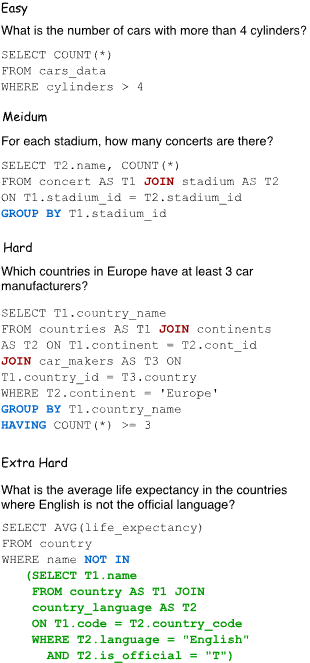
\includegraphics[width=0.35\textwidth]{image.png}
\caption{SQL query examples in 4 hardness levels. Credit: Spider [1]}
\label{fig:hardness-levels}
\end{figure}

\subsection{Prompting and Input}
\label{sec:prompting}

Each model receives three pieces of information in a single zero-shot user turn: a system instruction explaining its role as a Text-to-SQL generator, the database schema (table names, column names, primary keys, and foreign-key relationships, with no example rows), and the natural-language question. No few-shot examples are provided, so that the experiment measures each model's ability to generate SQL from instructions and schema information alone, without the confound of examples steering its output style. The prompt template is identical across all three models, so that differences in performance can be attributed to the models rather than to differences in prompting.

\textbf{Prompt template:}
\begin{verbatim}
Given the following SQLite database schema, write a SQL query that answers
the question.

{schema}

Question: {question}

Respond with only the SQL query in a ```sql code block.
\end{verbatim}

See \hyperref[sec:appendix1]{Appendix 1} for a worked example: a full schema, a question, and the resulting filled prompt.

\subsection{SQL Extraction}
\label{sec:sql-extraction}

For each sample, we decode the model's generated tokens into text using the model-specific tokenizer, and check for the presence of a \texttt{</think>} token. If \texttt{</think>} was generated, we take all text generated before \texttt{</think>} as the reasoning trace and all text to the right as the output SQL; DeepSeek-R1-Distill-Qwen-1.5B is the only model of the three that can emit this token. The SQL is then extracted from the first \texttt{```sql} code block in that remaining text. The extracted SQL is passed to the evaluation script as-is. Outputs that cannot be extracted or parsed are counted as incorrect on every metric rather than excluded from the evaluation, as unusable output is a task failure (see \ref{sec:evaluation-metrics} and \ref{sec:invalid-outputs}).

\subsection{Inference Settings}
\label{sec:inference-settings}

All models are evaluated using the same decoding configuration: greedy decoding (temperature and top-p are not applicable) for consistent, reproducible results between runs. The maximum output length differs by model: 256 tokens for Qwen3-0.6B, and 4096 tokens for both Qwen3-4B and DeepSeek-R1-Distill-Qwen-1.5B. For DeepSeek, the larger budget is needed because its output also has to contain a full reasoning trace rather than only the SQL query; Qwen3-4B is given the same, larger budget as DeepSeek so that a tighter token limit can be ruled out as the reason for any difference between them on invalid-output rate (\ref{sec:invalid-outputs}) or inference time (\ref{sec:efficiency}). Qwen3-0.6B and Qwen3-4B are both run with thinking mode off (both support it). DeepSeek-R1-Distill-Qwen-1.5B always produces a reasoning trace and has no documented way to disable thinking mode, so it is evaluated as the reasoning condition against the two non-reasoning Qwen3 models. All inference runs on the same 1x RTX 4090 GPU described in \ref{sec:models}, with batch size 1.

\subsection{Evaluation}
\label{sec:evaluation-metrics}

We evaluate the output using the same metrics as the Spider paper [1]. These are:

\begin{enumerate}
\item Component Matching
    \begin{itemize}
        \item For each of the following components:
        \begin{itemize}
            \item SELECT
            \item WHERE
            \item GROUP BY
            \item ORDER BY
            \item KEYWORDS (including all SQL keywords without column names and operators)
        \end{itemize}
        \item Decompose each component in the prediction and ground truth as bags of several sub-components and check whether or not these two sets of components match completely.
        \item Checks accuracy, recall, and F1
    \end{itemize}
\item Exact Matching Accuracy
    \begin{itemize}
        \item We measure whether the generated query as a whole is equivalent to the last section
        \item The generated query is correct only if all components are correct
        \item Checks only accuracy
    \end{itemize}
\item Execution Accuracy
    \begin{itemize}
        \item A list of gold values for each question is given
        \item We measure how many gold values the generated query extracts when executed
        \item Checks only accuracy
    \end{itemize}
\end{enumerate}

If output is invalid or unparsable, then it fails all 3 dimensions (component matching, exact matching, execution accuracy), consistent with how \ref{sec:sql-extraction} extracts and passes SQL to this evaluation script. This is reasonable as invalid/unparsable output cannot be applied to SQL and thus must be avoided and penalized heavily; Results~\ref{sec:invalid-outputs} reports how often this happens for each model.

\section{Task 1 -- RQ1: Results}
\label{sec:rq1-results}

\subsection{Overall Model Performance}
\label{sec:overall-performance}

Below we report how Qwen3-0.6B, Qwen3-4B, and Deepseek-R1-Distill-Qwen3-1.5B perform on the Spider benchmark across all 3 metrics (Component Matching, Exact Matching Accuracy, Execution Accuracy). We calculate the values per problem difficulty as well as overall, and display them in the below tables.

\begin{table}[H]
\centering
\footnotesize
\caption{Overall performance summary, aggregated across all difficulties (all 1034 problems). Component matching is accuracy / recall / F1 (macro-averaged, see the note on table~\ref{tab:difficulty-component} in \ref{sec:rq1-interpretation}). Per-difficulty breakdowns are in tables~\ref{tab:difficulty-component}--\ref{tab:difficulty-execution}.}
\label{tab:overall-performance}
\resizebox{\textwidth}{!}{%
\begin{tabular}{lllccc}
\toprule
Model & Parameters & Category & Component matching & Exact matching & Execution accuracy \\
\midrule
Qwen3-0.6B & 0.6B & Decoder-only & 0.628 / 0.209 / 0.314 & 0.099 & 0.209 \\
Qwen3-4B & 4B & Decoder-only & 0.797 / 0.306 / 0.442 & 0.256 & 0.353 \\
DeepSeek-R1-Distill-Qwen-1.5B & 1.5B & Reasoning & 0.661 / 0.174 / 0.275 & 0.085 & 0.121 \\
\bottomrule
\end{tabular}}
\end{table}

All models are evaluated zero-shot with the same prompt on the 20 databases of the Spider dev set. Aggregated across all difficulties and databases, every model is still far from solving the task: execution accuracy ranges from 0.121 (DeepSeek) to 0.353 (Qwen3-4B) and exact matching accuracy from 0.085 (DeepSeek) to 0.256 (Qwen3-4B). Execution accuracy is higher than exact matching accuracy for all three models (for example 0.353 vs.\ 0.256 for Qwen3-4B), which suggests that at least some of the queries that return the correct result are written differently from the gold SQL (see \ref{sec:rq1-interpretation} for more on this relationship). Of the three models, Qwen3-4B is now the best on almost every metric, database, and difficulty level; \ref{sec:by-database} and \ref{sec:rq1-interpretation} quantify how consistently. Table~\ref{tab:inference-time} reports the efficiency side of this comparison: inference time per example.

\subsection{Performance by Query Difficulty}
\label{sec:by-difficulty}

\begin{table}[H]
\centering
\footnotesize
\caption{Component matching (accuracy / recall / F1) by difficulty.}
\label{tab:difficulty-component}
\begin{tabular}{lcc}
\toprule
Model & easy & medium \\
\midrule
Problems (n) & 248 & 446 \\
Qwen3-0.6B & 0.675 / 0.308 / 0.423 & 0.582 / 0.235 / 0.334 \\
Qwen3-4B & 0.838 / 0.574 / 0.681 & 0.670 / 0.306 / 0.420 \\
DeepSeek-R1-Distill-Qwen-1.5B & 0.566 / 0.288 / 0.382 & 0.642 / 0.185 / 0.287 \\
\bottomrule
\end{tabular}

\vspace{0.5em}

\begin{tabular}{lccc}
\toprule
Model & hard & extra & all \\
\midrule
Problems (n) & 174 & 166 & 1034 \\
Qwen3-0.6B & 0.540 / 0.141 / 0.223 & 0.578 / 0.160 / 0.250 & 0.628 / 0.209 / 0.314 \\
Qwen3-4B & 0.796 / 0.262 / 0.394 & 0.485 / 0.150 / 0.229 & 0.797 / 0.306 / 0.442 \\
DeepSeek-R1-Distill-Qwen-1.5B & 0.543 / 0.113 / 0.187 & 0.389 / 0.104 / 0.164 & 0.661 / 0.174 / 0.275 \\
\bottomrule
\end{tabular}
\end{table}

\begin{table}[H]
\centering
\footnotesize
\caption{Exact matching accuracy by difficulty.}
\label{tab:difficulty-exact}
\begin{tabular}{lccccc}
\toprule
Model & easy & medium & hard & extra & all \\
\midrule
Problems (n) & 248 & 446 & 174 & 166 & 1034 \\
Qwen3-0.6B & 0.157 & 0.137 & 0.006 & 0.006 & 0.099 \\
Qwen3-4B & 0.508 & 0.262 & 0.115 & 0.012 & 0.256 \\
DeepSeek-R1-Distill-Qwen-1.5B & 0.214 & 0.078 & 0.000 & 0.000 & 0.085 \\
\bottomrule
\end{tabular}
\end{table}

\begin{table}[H]
\centering
\footnotesize
\caption{Execution accuracy by difficulty.}
\label{tab:difficulty-execution}
\begin{tabular}{lccccc}
\toprule
Model & easy & medium & hard & extra & all \\
\midrule
Problems (n) & 248 & 446 & 174 & 166 & 1034 \\
Qwen3-0.6B & 0.210 & 0.276 & 0.126 & 0.114 & 0.209 \\
Qwen3-4B & 0.565 & 0.345 & 0.276 & 0.139 & 0.353 \\
DeepSeek-R1-Distill-Qwen-1.5B & 0.258 & 0.128 & 0.017 & 0.006 & 0.121 \\
\bottomrule
\end{tabular}
\end{table}

We break every metric down by the Spider Hardness Criteria (\ref{sec:eval-data}) as query difficulty is a first-order driver of Text-to-SQL performance; comparing models only in aggregate would hide whether a model's advantage holds up as queries get harder.

Performance decreases with difficulty for every model, but the decrease is steepest for Qwen3-0.6B and DeepSeek: their exact matching and execution accuracy are both at most 0.034 and 0.126 respectively on hard and extra problems, down from as high as 0.210-0.258 (easy execution) on the easiest problems (table~\ref{tab:difficulty-exact} and table~\ref{tab:difficulty-execution}). Qwen3-4B degrades on the same relative scale but from a much higher starting point, from 0.508 easy exact matching / 0.565 easy execution accuracy down to 0.012 extra exact matching / 0.139 extra execution accuracy. Despite the degredation, it remains the best of the three models at every single difficulty level on both metrics (tables~\ref{tab:difficulty-exact}--\ref{tab:difficulty-execution}).

\subsection{Performance by Database}
\label{sec:by-database}

We also break execution and exact matching accuracy down by each of the 20 Spider dev databases. Qwen3-4B has the highest execution accuracy on 17 of the 20 databases outright (plus a tie on one more) and the highest exact matching accuracy on 18 of 20, while DeepSeek-R1-Distill-Qwen-1.5B is never highest on either metric; Qwen3-0.6B wins outright only on orchestra and battle\_death. Databases with few problems (real\_estate\_properties with n=4, voter\_1 with n=15, battle\_death with n=16, and museum\_visit with n=18) are too small to rank the models reliably, since a single problem changes a score by 6 to 25 percentage points. Execution accuracy ranges from 0.10 (course\_teach) to 0.53 (singer) for Qwen3-0.6B, from 0.19 (battle\_death) to 0.60 (singer) for Qwen3-4B, and from 0.00 (concert\_singer) to 0.27 (singer and voter\_1) for DeepSeek-R1-Distill-Qwen-1.5B (\hyperref[tab:db-execution]{Table 5}). The pattern on exact matching accuracy is just as one-sided (\hyperref[tab:db-exact]{Table 6}): Qwen3-4B is highest on 18 of 20 databases, ties Qwen3-0.6B on orchestra, and loses only on battle\_death; DeepSeek's exact matching accuracy is never the highest of the three, coming closest on flight\_2 (0.200 vs.\ Qwen3-4B's 0.350 and Qwen3-0.6B's 0.075). The full per-database tables and discussion are in \hyperref[sec:appendix2]{Appendix 2}.

\subsection{Invalid and Unparseable Outputs}
\label{sec:invalid-outputs}

We also count how often each model's output cannot be used as SQL at all: it either never produces a usable query within the token budget (\ref{sec:inference-settings}) or is truncated before finishing one. Per \ref{sec:evaluation-metrics}, these count as failures on every metric rather than being excluded, and this is a direct measure of how reliably each model follows the ``respond with only a SQL query'' instruction, independent of whether the SQL it does produce is correct. Qwen3-0.6B's invalid rate is 2.2\%, Qwen3-4B's is 0.0\%, and DeepSeek-R1-Distill-Qwen-1.5B's is 9.7\%, about 4x higher than Qwen3-0.6B's despite having the same 4096-token budget as Qwen3-4B (\ref{sec:inference-settings}), i.e. a larger token budget did not cause Qwen3-4B to run on or produce unusable output the way it does for DeepSeek. \ref{sec:rq1-interpretation} breaks DeepSeek's failures down further by difficulty and by why the generation failed (tables~\ref{tab:deepseek-outcome}--\ref{tab:deepseek-unfinished-by-difficulty}).

\subsection{Efficiency Measures}
\label{sec:efficiency}

\begin{table}[H]
\centering
\footnotesize
\caption{Output tokens per example}
\label{tab:tokens-per-example}
\begin{tabular}{lccccc}
\toprule
Model & easy & medium & hard & extra & all \\
\midrule
Qwen3-0.6B & 27.5 & 44.7 & 53.7 & 69.9 & 46.1 \\
Qwen3-4B & 23.6 & 37.3 & 46.2 & 59.0 & 39.0 \\
DeepSeek-R1-Distill-Qwen-1.5B & 610.8 & 768.4 & 1096.0 & 1176.9 & 851.3 \\
\bottomrule
\end{tabular}
\end{table}

Inference time is measured from the start of generation to the complete batch output, per batch of 1 example, excluding tokenization, model loading, and warm-up.

\begin{table}[H]
\centering
\footnotesize
\caption{Inference time.}
\label{tab:inference-time}
\begin{tabular}{lcc}
\toprule
Model & Total wall time (s) & Avg.\ time per example (s) \\
\midrule
Qwen3-0.6B & 123.9 & 0.120 \\
Qwen3-4B & 109.1 & 0.106 \\
DeepSeek-R1-Distill-Qwen-1.5B & 3059.8 & 2.959 \\
\bottomrule
\end{tabular}
\end{table}

DeepSeek is about 25x slower per example than Qwen3-0.6B and 28x slower than Qwen3-4B, consistent with its much higher average token count (table~\ref{tab:tokens-per-example}). Qwen3-4B, despite having about 7x as many parameters as Qwen3-0.6B, is marginally faster per example (0.106s vs.\ 0.120s), consistent with it generating fewer tokens on average (39.0 vs.\ 46.1, table~\ref{tab:tokens-per-example}) despite having the same 16x larger token budget as DeepSeek (\ref{sec:inference-settings}).

\begin{table}[H]
\centering
\footnotesize
\caption{DeepSeek-R1-Distill-Qwen-1.5B by generation outcome. ``Cut'' means the generation reached the 4096-token limit.}
\label{tab:deepseek-outcome}
\begin{tabular}{lccccc}
\toprule
Outcome & Problems (n) & Share & Avg.\ tokens & Exact match & Component F1 \\
\midrule
Finished with SQL & 934 & 90.3\% & 512 & 0.094 & 0.286 \\
Finished, no usable SQL & 2 & 0.2\% & 284 & 0.000 & 0.100 \\
Cut while answering (after \texttt{</think>}) & 13 & 1.3\% & 4096 & 0.000 & 0.096 \\
Cut while thinking (no \texttt{</think>}) & 85 & 8.2\% & 4096 & 0.000 & 0.093 \\
All & 1034 & 100\% & 851 & 0.085 & 0.275 \\
\bottomrule
\end{tabular}
\end{table}

\begin{table}[H]
\centering
\footnotesize
\caption{The same 934 questions that DeepSeek finished, for all three models.}
\label{tab:deepseek-finished-934}
\begin{tabular}{lcc}
\toprule
Model & Exact match & Component F1 \\
\midrule
DeepSeek-R1-Distill-Qwen-1.5B & 0.094 & 0.286 \\
Qwen3-0.6B & 0.103 & 0.317 \\
Qwen3-4B & 0.257 & 0.440 \\
\bottomrule
\end{tabular}
\end{table}

\begin{table}[H]
\centering
\footnotesize
\caption{Are the cut-off DeepSeek generations infinite self-repetition loops? A text that repeats itself compresses well, so a low compression ratio of the last 3000 characters indicates a loop.}
\label{tab:deepseek-repetition}
\begin{tabular}{lcccc}
\toprule
Generations & n & Median compression ratio & Ratio $<$ 0.15 & Last 150 characters repeat 3 or more times \\
\midrule
Cut off & 98 & 0.095 & 95.9\% & 96.9\% \\
Finished & 936 & 0.418 & 0.0\% & 0.2\% \\
\bottomrule
\end{tabular}
\end{table}

\begin{table}[H]
\centering
\footnotesize
\caption{Share of DeepSeek generations that did not finish with SQL, by difficulty.}
\label{tab:deepseek-unfinished-by-difficulty}
\begin{tabular}{lccccc}
\toprule
 & easy & medium & hard & extra & all \\
\midrule
Problems (n) & 248 & 446 & 174 & 166 & 1034 \\
Not finished with SQL (n) & 15 & 33 & 25 & 27 & 100 \\
Share & 6.0\% & 7.4\% & 14.4\% & 16.3\% & 9.7\% \\
\bottomrule
\end{tabular}
\end{table}

\section{Interpretation and Answer to Research Question (RQ1)}
\label{sec:rq1-interpretation}

\textbf{RQ1:} How do (selected) LLMs perform on cross-domain Text-to-SQL?

\vspace{10px}

All three models are still far from solving the task in this zero-shot setting: exact matching accuracy ranges from 0.085 to 0.256 and execution accuracy from 0.121 to 0.353 (table~\ref{tab:overall-performance}). Difficulty and database effects are discussed in \ref{sec:by-difficulty} and \ref{sec:by-database}; here we interpret the effects of model size and reasoning architecture and the exact-match/execution-accuracy relationship, and state the answer to RQ1 as three findings.

\textbf{First, within the Qwen family, scale is a strong and almost uniform predictor of performance, but an intermediate-size reasoning model from the Deepseek family still loses to the smallest model in the Qwen family.} Aggregated across all difficulties, Qwen3-4B has the best component matching (0.797 / 0.306 / 0.442), exact matching (0.256), and execution accuracy (0.353) of the three (table~\ref{tab:overall-performance}), and it beats Qwen3-0.6B on exact matching and execution accuracy at every individual difficulty level, including hard (0.115 vs.\ 0.006) and extra (0.012 vs.\ 0.006), where the smaller model solves almost nothing (tables~\ref{tab:difficulty-exact}--\ref{tab:difficulty-execution}). This is the largest, most consistent effect in the RQ1 results. The one exception is component matching on extra-hard problems, where Qwen3-0.6B's accuracy, recall, and F1 (0.578 / 0.160 / 0.250) are all slightly higher than Qwen3-4B's (0.485 / 0.150 / 0.229), the only point in the RQ1 results where the smaller Qwen3 model wins outright (table~\ref{tab:difficulty-component}). DeepSeek-R1-Distill-Qwen-1.5B sits between the two Qwen3 models in parameter count (1.5B) and is the only one that reasons, yet it is the lowest of the three on every aggregate metric (0.275 component F1, 0.085 exact matching, 0.121 execution accuracy) except its own component-matching accuracy (0.661 vs.\ 0.628 for Qwen3-0.6B). Thus, scale predicts performance well within a family, but does not transfer across the reasoning/non-reasoning boundary: having more parameters than Qwen3-0.6B did not help DeepSeek catch up to it.

\textbf{Second, the reasoning architecture itself, not parameter count, is the main driver of DeepSeek's low score.} Its invalid-output rate (9.7\%) is markedly higher than Qwen3-0.6B's (2.2\%) and Qwen3-4B's (0.0\% in this run) (\ref{sec:invalid-outputs}). In tables~\ref{tab:deepseek-outcome}--\ref{tab:deepseek-unfinished-by-difficulty}, 100 of 1034 generations (9.7\%) end without usable SQL. 85 never leave the reasoning phase, 13 are cut while writing the answer, and 2 finish without SQL. The number of unusable SQL generations also grows with difficulty, from 6.0\% on easy to 16.3\% on extra problems. These are not cases of long productive reasoning either: 95.9\% of the cut-off generations are highly self-repetitive (compression ratio below 0.15, median compression ratio 0.095, vs.\ 0.418 for finished generations), rewriting the same query and repeating phrases like ``So the final query is:'' without converging. Finishing does not make it better either: on the 934 questions DeepSeek does finish, its exact matching (0.094) and component F1 (0.286) are still below Qwen3-0.6B's on the same questions (0.103 / 0.317) and far below Qwen3-4B's (0.257 / 0.440), despite generating 512 tokens per question on average there, against 46 and 39 tokens overall for Qwen3-0.6B and Qwen3-4B (about 18x and 22x fewer). This extra length also costs time: DeepSeek is 25-28x slower per example than either Qwen3 model (\ref{sec:efficiency}). The reasoning trace mostly lengthens the output and sometimes never terminates, without improving the SQL when it does, and size alone is not the explanation, since Qwen3-4B is both bigger than DeepSeek and the best model in the comparison. Thus, reasoning architecture itself, not the parameter count, is the main driver of DeepSeek's low score.

\textbf{Third, query difficulty has a substantial, consistent effect on every model, including the best one.} Exact matching and execution accuracy both fall sharply from easy to extra-hard problems for all three models (\ref{sec:by-difficulty}). Qwen3-4B's drop is from a much higher base (0.508 to 0.012 exact matching, 0.565 to 0.139 execution accuracy) and it remains the best model at every difficulty level on both metrics, but the drop itself is just as steep in relative terms as for the other two models, and the hardest problems remain largely unsolved even for it.

\textbf{Exact match vs.\ execution accuracy.} For all three models, execution accuracy aggregated across all difficulties exceeds exact matching accuracy (table~\ref{tab:overall-performance}): 0.209 vs.\ 0.099 for Qwen3-0.6B, 0.353 vs.\ 0.256 for Qwen3-4B, and 0.121 vs.\ 0.085 for DeepSeek. Since exact matching requires every SQL component to match the gold query while execution accuracy only requires the same result set, this gap indicates each model writes some queries that are valid and correct but phrased differently from the gold SQL (e.g.\ a different but equivalent join order, or an explicit column list where the gold query uses \texttt{SELECT *}). The gap is widest for Qwen3-0.6B (11.0 points), close behind for Qwen3-4B (9.7 points), and narrowest for DeepSeek (3.6 points); DeepSeek's narrower gap reflects it producing fewer alternative-but-valid queries. Qwen3-4B's gap is almost as wide as Qwen3-0.6B's despite much higher absolute accuracy, so scaling up within the Qwen3 family raises both Exact Match Accuracy and Execution Accuracy together rather than closing the gap between them.

\textbf{Limitations.} Our working hypothesis is that Text-to-SQL at this scale does not benefit from an explicit reasoning trace, and that a non-reasoning model is sufficient, with performance instead scaling with parameter count within a fixed model family. The results are consistent with this hypothesis. However, they do not establish that Text-to-SQL is too simple for reasoning models in general due to several factors:

\begin{itemize}
\item \textbf{Truncation and failed outputs for DeepSeek.} These count as failures on every metric and lower its recall, exact matching, and execution scores, but table~\ref{tab:deepseek-finished-934} shows removing them would not change the ranking (DeepSeek is also lower on the questions it finished), and table~\ref{tab:deepseek-repetition} shows the cut-off generations are repetition loops, so a larger token budget is unlikely to rescue them.
\item \textbf{Model differences beyond reasoning.} Qwen3-0.6B and Qwen3-4B share a model family, isolating the effect of scale between them, but DeepSeek differs from both in family, size, and pretraining/post-training, not only in whether it reasons; it is also a distilled model, so the effect of reasoning cannot be fully separated from distillation quality.
\item \textbf{Aggregated component matching.} The component matching figures in table~\ref{tab:difficulty-component} (and in table~\ref{tab:overall-performance}) are our own macro-average (mean of the 10 per-component accuracy and recall scores, with F1 computed from these two means), not a number reported by Spider.
\end{itemize}

Overall, in this zero-shot, cross-domain setting, a larger non-reasoning decoder-only model (Qwen3-4B, 4B) clearly outperforms both a same-family model at under a sixth its size (Qwen3-0.6B) and a reasoning model of intermediate size from a different family (DeepSeek-R1-Distill-Qwen-1.5B, 1.5B), while also being faster per example than either. None of the three models solve more than half of even the easiest problems or more than a small fraction of hard or extra-hard queries. This answers RQ1 for the three models evaluated.
 (this
% file's cross-references into Task 1 -- table~\ref{tab:deepseek-outcome},
% \ref{tab:tokens-per-example}, \ref{sec:sql-extraction}, etc. -- rely on
% RQ1.tex's labels already being defined earlier in the same document).
%
% Structure: Methodology is organized per-feature (Feature 1: Token Count,
% Feature 2: Information Retention), each with its own Definition / Why it's
% relevant / How we computed it. Results is organized as descriptive
% statistics, differences by correctness, differences by difficulty, and
% relationship with Text-to-SQL correctness (the correlation analysis).

\section{Task 2 -- RQ2: Methodology}
\label{sec:rq2-methodology}

\textbf{RQ2:} How do characteristics of reasoning traces (of reasoning LLM) relate to Text-to-SQL performance?

To answer this question, we examine two features of each reasoning trace: Token Count and Information Retention. We compute both for all 1034 generations in DeepSeek-R1-Distill-Qwen-1.5B's main Task 1 run, then relate each to difficulty and to Text-to-SQL correctness.

\subsection{Feature 1: Token Count}
\label{sec:rq2-feature-tokencount}

\textbf{Definition.} Token Count is the number of tokens in the reasoning segment of a generation, i.e.\ everything the model generates before \texttt{</think>}, excluding the final SQL answer. We split each generation into a reasoning segment and an answer segment using the same \texttt{</think>} split used in Task 1 (\ref{sec:sql-extraction}).

\textbf{Why it's relevant.} We expect Token Count to scale positively with the difficulty of the related Text-to-SQL problem: easy questions should require fewer thinking tokens, while extra-hard questions should require significantly more. Any question that disobeys this relation, or where more tokens associate with worse rather than better answers, is given special attention in Results. Token Count is also the most direct, model-agnostic proxy we have for how much deliberation went into an answer, so it is a natural first feature to test against correctness.

\textbf{How we computed it.} Token Count is the number of tokens in the reasoning segment only, re-tokenized with the model's own tokenizer (not the \texttt{new\_tokens} field logged during generation, which counts the whole generation, reasoning plus SQL). For generations that never emit \texttt{</think>} (truncated at the 4096-token generation limit, see Task 1's table~\ref{tab:deepseek-outcome}), the entire generated text is treated as the reasoning segment, so Token Count for these rows is effectively capped at the generation limit rather than reflecting a completed thought. This is intentional: these cases are exactly the repetition loops Task 1 identified (table~\ref{tab:deepseek-repetition}), and dropping them would hide, rather than explain, the heavy right tail in Token Count. We keep them in the Token Count analysis and flag wherever they drive a result (see finding~\ref{item:rq2-finding-tokencount-difficulty} in Results).

\begin{table}[H]
\centering
\footnotesize
\caption{Token Count: definition and computation summary.}
\label{tab:rq2-feature-tokencount-summary}
\begin{tabular}{p{0.22\textwidth}p{0.7\textwidth}}
\toprule
Property & Detail \\
\midrule
Unit & Tokens (model's own tokenizer) \\
Scope & Reasoning segment only, i.e.\ text before \texttt{</think>} \\
Range & Non-negative integer, long right tail (observed 103--4166) \\
Truncated traces & Treated as reasoning segment in full; capped at the 4096-token generation limit \\
Hypothesis & Increases with difficulty; should not correlate with worse correctness \\
Test & Spearman's rank correlation vs.\ difficulty and vs.\ 32 per-question performance submetrics \\
\bottomrule
\end{tabular}
\end{table}

\subsection{Feature 2: Information Retention}
\label{sec:rq2-feature-retention}

\textbf{Definition.} Information Retention is the share of schema-shaped identifiers mentioned in a reasoning trace that actually exist as a table or column name in that question's schema. Equivalently, $1 - $ Information Retention is the hallucination rate of the trace: the fraction of mentioned identifiers that are not grounded in the prompt.

\textbf{Why it's relevant.} We expect reasoning traces with low Information Retention (frequent hallucination of schema elements) to produce lower-performing answers than traces that stay grounded in the given schema, since inventing a table or column that doesn't exist is very likely to propagate into an incorrect query. We also expect harder problems to not cause lower Information Retention on their own; if they do, this points to the model introducing more assumptions as questions get harder, which is itself worth investigating as a bias rather than attributing the accuracy drop to difficulty alone.

\textbf{How we computed it.} We regex-extract every schema-shaped identifier the trace mentions, either quoted (e.g.\ \texttt{"Singer\_ID"}) or underscore-joined (e.g.\ \texttt{concert\_id}), and take the share of those identifiers that match a table or column name in that question's schema. An identifier that matches neither is treated as a fact the model introduced on its own, i.e., a hallucination. Traces that mention no schema identifiers at all are excluded from Information Retention (but kept for Token Count), since a 0-of-0 ratio is undefined rather than evidence of perfect or zero retention; this drops the usable sample from 1034 to 1017. Truncated traces are scored the same way, over whatever partial text was generated.

\begin{table}[H]
\centering
\footnotesize
\caption{Information Retention: definition and computation summary.}
\label{tab:rq2-feature-retention-summary}
\begin{tabular}{p{0.22\textwidth}p{0.7\textwidth}}
\toprule
Property & Detail \\
\midrule
Unit & Ratio, bounded in $[0,1]$ \\
Numerator & Schema identifiers mentioned in the trace that match a real table/column name \\
Denominator & All schema-shaped identifiers mentioned in the trace (quoted or underscore-joined) \\
Exclusions & Traces mentioning zero schema identifiers (1034 $\rightarrow$ 1017 usable rows) \\
Truncated traces & Scored over the partial text generated before truncation \\
Hypothesis & Higher retention associates with better correctness; should not fall with difficulty \\
Test & Spearman's rank correlation vs.\ difficulty and vs.\ 32 per-question performance submetrics \\
\bottomrule
\end{tabular}
\end{table}

\subsection{Statistical approach}
\label{sec:rq2-statistical-approach}

We relate both Token Count and Information Retention to correctness and difficulty with Spearman's Rank Correlation throughout. Both of our hypotheses are about monotonic relationships, not linear relationships (performance should not decrease as Token Count or Information Retention increase, and Token Count should increase with difficulty), which is exactly what Spearman's Rank Correlation tests for. It also suits the distribution of our two reasoning metrics: Token Count is a non-negative count with a long right tail (DeepSeek alone ranges from 611 tokens on easy problems to 1177 on extra, table~\ref{tab:tokens-per-example}), and Information Retention is a bounded ratio, so neither is likely to be symmetric and unbounded; the $\geq$90\% trace completion rate gives us enough data per stratum to check this on histograms rather than assume it. For correctness, we correlate each reasoning metric against the continuous, per-question component matching accuracy, recall, and F1 for all ten Spider components individually, plus exact matching and execution accuracy, rather than collapsing them into one pass/fail label, which keeps the per-question variance in performance a binary cutoff would discard and sidesteps splitting by correctness directly, which is not viable per difficulty level: DeepSeek's exact matching accuracy falls to at most 0.034 on hard and extra problems, leaving as few as four to six correct traces in those strata. This gives 32 submetrics per reasoning metric per difficulty level. We chose this rank-based, continuous-correlation approach over a parametric correlation or a correct/incorrect group comparison because our data is too skewed for the former and our correct-answer strata too sparse for the latter. With 169 correlation tests run in total, we correct for multiple comparisons with the Benjamini-Hochberg procedure rather than a stricter family-wise correction like Bonferroni: we are screening many related, non-independent submetrics for the strongest associations to report and discuss, not making a small number of pre-registered confirmatory claims, so controlling the expected false-discovery rate is a better fit than controlling the probability of any single false positive at the cost of statistical power.

The Results below report Token Count and Information Retention broken down two ways: by difficulty, since that is the primary hypothesis under test, and by exact-match correctness (correct/incorrect), used for the descriptive statistics and the boxplots (figure~\ref{fig:rq2-boxplots}) because a binary split is easier to read in a table or figure than 32 continuous submetrics. The correlation analysis itself (table~\ref{tab:rq2-correlations}) still uses the continuous submetrics described above, for the statistical-power reasons given there; the binary-correctness view and the continuous-submetric view are two presentations of the same underlying data, not two different analyses.

\textbf{Verification.} To check that the Spearman findings above are not artifacts of one particular rank-based method or of an unmodeled confound, we add two further layers of testing, reported in \ref{sec:rq2-verification} and \ref{sec:rq2-robustness}. First, we run two confirmatory, feature-specific significance tests directly on the binary/ordinal views used for the descriptive statistics: a Mann-Whitney U test for each feature against exact-match correctness (overall and within each difficulty stratum), and Kendall's tau-b for each feature against difficulty (overall and within each correctness stratum). We prefer Kendall's tau-b over a second Spearman run here because it is the standard choice when one variable has many ties (difficulty has only four distinct values, and Information Retention has a large tied mass at 1.0), and it is the ordered-groups analogue of the Jonckheere-Terpstra trend test. Second, because Token Count, Information Retention and difficulty are all correlated with one another, a bivariate relationship between one feature and an outcome could simply be riding on the other two variables rather than reflecting an independent association. We fit two regression models to check this: a logistic regression of exact-match correctness on standardized log Token Count, standardized Information Retention, and standardized difficulty, all entered jointly; and a proportional-odds (ordinal) regression of difficulty on standardized log Token Count and standardized Information Retention, entered jointly. Token Count is log-transformed before standardizing given its heavy right skew (see above); difficulty enters the logistic model as a single linear control on the log-odds scale, which is a simplification rather than a full categorical treatment, and the ordinal model assumes proportional odds across the three difficulty thresholds, which we did not separately test -- both are limitations of this robustness check, not of the primary Spearman analysis. All four verification tests and both regression models are implemented in \texttt{eval/evalpipeline/reasoning\_verification.py}, run on the same per-question table as the Spearman analysis.

\section{Task 2 -- RQ2: Results}
\label{sec:rq2-results}

We compute Token Count and Information Retention for all 1034 generations in DeepSeek-R1-Distill-Qwen-1.5B's main Task 1 run, and correlate each against difficulty and against all 32 per-question performance submetrics as described in the Methodology. Table~\ref{tab:rq2-descriptive-stats-tokencount} and table~\ref{tab:rq2-descriptive-stats-retention} give descriptive statistics for each feature by difficulty and by exact-match correctness; figure~\ref{fig:rq2-boxplots} shows the resulting distributions; table~\ref{tab:rq2-correlations} lists the strongest correlations.

\subsection{Descriptive statistics}
\label{sec:rq2-descriptive-stats}

\begin{table}[H]
\centering
\footnotesize
\caption{Token Count descriptive statistics, by difficulty and by exact-match correctness (1 = exact match, 0 = not). Full results in \texttt{eval/results/task2\_analysis/descriptive\_stats.csv}.}
\label{tab:rq2-descriptive-stats-tokencount}
\begin{tabular}{lcccccc}
\toprule
Group & n & mean & median & std & min & max \\
\midrule
easy & 248 & 542.3 & 329.0 & 845.2 & 103 & 4096 \\
medium & 446 & 648.2 & 374.0 & 925.7 & 191 & 4166 \\
hard & 174 & 939.2 & 425.0 & 1246.2 & 226 & 4096 \\
extra & 166 & 901.6 & 434.5 & 1199.9 & 222 & 4096 \\
\midrule
exact match = 0 & 946 & 748.1 & 394.0 & 1065.6 & 103 & 4166 \\
exact match = 1 & 88 & 329.3 & 314.5 & 97.7 & 195 & 849 \\
\midrule
all & 1034 & 712.4 & 383.0 & 1026.2 & 103 & 4166 \\
\bottomrule
\end{tabular}
\end{table}

\begin{table}[H]
\centering
\footnotesize
\caption{Information Retention descriptive statistics, by difficulty and by exact-match correctness (1 = exact match, 0 = not). Excludes traces that mention no schema identifiers (n drops from 1034 to 1017 overall). Full results in \texttt{eval/results/task2\_analysis/descriptive\_stats.csv}.}
\label{tab:rq2-descriptive-stats-retention}
\begin{tabular}{lcccccc}
\toprule
Group & n & mean & median & std & min & max \\
\midrule
easy & 246 & 0.915 & 1.0 & 0.146 & 0.0 & 1.0 \\
medium & 441 & 0.905 & 1.0 & 0.148 & 0.0 & 1.0 \\
hard & 172 & 0.877 & 1.0 & 0.163 & 0.0 & 1.0 \\
extra & 158 & 0.861 & 1.0 & 0.215 & 0.0 & 1.0 \\
\midrule
exact match = 0 & 931 & 0.893 & 1.0 & 0.166 & 0.0 & 1.0 \\
exact match = 1 & 86 & 0.924 & 1.0 & 0.123 & 0.5 & 1.0 \\
\midrule
all & 1017 & 0.896 & 1.0 & 0.163 & 0.0 & 1.0 \\
\bottomrule
\end{tabular}
\end{table}

\begin{figure}[H]
\centering
\includegraphics[width=0.95\textwidth]{boxplots.png}
\caption{Token Count and Information Retention by difficulty and by exact-match correctness, for DeepSeek-R1-Distill-Qwen-1.5B's 1034 Task 1 generations. Green triangles are means, orange lines are medians. Means sit well above medians throughout, confirming the right-skewed, bounded distributions the Methodology assumes rather than normal ones.}
\label{fig:rq2-boxplots}
\end{figure}

\subsection{Differences by correctness}
\label{sec:rq2-by-correctness}

Correct generations (exact match = 1) have a much lower mean and tighter spread of Token Count (329.3, std 97.7) than incorrect ones (748.1, std 1065.6, table~\ref{tab:rq2-descriptive-stats-tokencount}), and a slightly higher mean Information Retention (0.924 vs.\ 0.893, table~\ref{tab:rq2-descriptive-stats-retention}). Both differences point the same direction as the correlation findings in \ref{sec:rq2-relationship-correctness}: more reasoning tokens and lower retention associate with worse performance. The gap is far larger for Token Count than for Information Retention: incorrect generations' Token Count std (1065.6) is more than ten times that of correct generations (97.7), driven by the truncated, repetition-loop traces described in \ref{sec:rq2-feature-tokencount}, almost none of which are exact matches. Information Retention's median is 1.0 in both correctness groups, so the correctness gap in retention lives entirely in the mean and the lower tail, not in a shift of the typical trace.

\subsection{Differences by difficulty}
\label{sec:rq2-by-difficulty}

\begin{enumerate}
\item \label{item:rq2-finding-tokencount-difficulty} \textbf{Token Count increases with difficulty, as hypothesized, but the increase is driven by a heavy tail.} Median token count rises from 329 (easy) to 374 (medium) to 425 (hard) to 434 (extra), and the correlation with difficulty is positive and significant ($\rho=0.313$, $q<0.001$). The mean rises faster than the median at every level (for example 542 vs.\ 329 on easy), because generations hitting the 4096-token limit occur at every difficulty (figure~\ref{fig:rq2-boxplots}, top row); these are the same repetition loops Task 1 identified, not productive extra reasoning on harder problems.
\item \label{item:rq2-finding-retention-difficulty} \textbf{Information Retention decreases slightly with difficulty.} Median retention is 1.0 at every difficulty level, but the mean falls from 0.915 (easy) to 0.861 (extra), and the correlation with difficulty is negative and significant ($\rho=-0.107$, $q=0.013$). Per the Methodology, this is the case that calls for examining the model's introduced assumptions on harder problems rather than attributing the accuracy drop to difficulty alone.
\end{enumerate}

\subsection{Relationship with Text-to-SQL correctness}
\label{sec:rq2-relationship-correctness}

\begin{enumerate}
\item \label{item:rq2-finding-tokencount-disobey} \textbf{On easy and medium problems, more Token Count tracks worse performance, the ``disobeying'' case flagged in the Methodology.} Token Count correlates negatively with \texttt{keywords} F1 on easy ($\rho=-0.42$, $q<0.001$) and medium ($\rho=-0.19$, $q=0.001$) problems, and with \texttt{where} and \texttt{where(no OP)} F1 on easy problems ($\rho=-0.32$ and $-0.33$, $q<0.001$). Combined with finding~\ref{item:rq2-finding-tokencount-difficulty}, the extra tokens on these problems look like run-away generation rather than helpful deliberation.
\item \label{item:rq2-finding-retention-performance} \textbf{Where Information Retention does relate to performance, it is positive, as hypothesized.} On medium problems, Information Retention correlates positively with \texttt{where} and \texttt{where(no OP)} F1 ($\rho=0.345$, $q<0.001$ for both), consistent with higher-retention traces producing more accurate WHERE clauses. Of the 169 tests run, 26 remain significant after Benjamini-Hochberg correction; the strongest are in table~\ref{tab:rq2-correlations}.
\end{enumerate}

\begin{table}[H]
\centering
\footnotesize
\caption{Strongest Spearman correlations between reasoning metrics and performance submetrics, Benjamini-Hochberg corrected, top 8 of 169 tests by q-value. Full results in \texttt{eval/results/task2\_analysis/spearman\_correlations.csv}.}
\label{tab:rq2-correlations}
\begin{tabular}{llcccc}
\toprule
Metric & Submetric & Difficulty & n & $\rho$ & $q$ \\
\midrule
Token Count & difficulty (overall) & all & 1034 & 0.313 & $<$0.001 \\
Information Retention & where F1 & medium & 441 & 0.345 & $<$0.001 \\
Information Retention & where(no OP) F1 & medium & 441 & 0.345 & $<$0.001 \\
Token Count & keywords F1 & easy & 248 & -0.417 & $<$0.001 \\
Token Count & where(no OP) F1 & easy & 248 & -0.332 & $<$0.001 \\
Token Count & where F1 & easy & 248 & -0.322 & $<$0.001 \\
Token Count & keywords F1 & medium & 446 & -0.194 & $<$0.001 \\
Information Retention & difficulty (overall) & all & 1017 & -0.107 & 0.013 \\
\bottomrule
\end{tabular}
\end{table}

\subsection{Verification: Mann-Whitney U and Kendall's tau-b}
\label{sec:rq2-verification}

\begin{table}[H]
\centering
\footnotesize
\caption{Mann-Whitney U test: Token Count by exact-match correctness, overall and within each difficulty stratum. $r$ is the rank-biserial correlation (negative = higher Token Count associates with incorrect answers). Full results in \texttt{eval/results/task2\_analysis/mann\_whitney\_tokencount.csv}.}
\label{tab:rq2-mw-tokencount}
\begin{tabular}{lccccc}
\toprule
Stratum & n(incorrect) & n(correct) & $U$ & $p$ & $r$ \\
\midrule
all & 946 & 88 & 60406.5 & $<$0.001 & -0.451 \\
easy & 195 & 53 & 6423.0 & 0.007 & -0.243 \\
medium & 411 & 35 & 9644.0 & 0.001 & -0.341 \\
hard & 174 & 0 & --- & --- & --- \\
extra & 166 & 0 & --- & --- & --- \\
\bottomrule
\end{tabular}
\end{table}

\begin{table}[H]
\centering
\footnotesize
\caption{Mann-Whitney U test: Information Retention by exact-match correctness, overall and within each difficulty stratum. Full results in \texttt{eval/results/task2\_analysis/mann\_whitney\_retention.csv}.}
\label{tab:rq2-mw-retention}
\begin{tabular}{lccccc}
\toprule
Stratum & n(incorrect) & n(correct) & $U$ & $p$ & $r$ \\
\midrule
all & 931 & 86 & 36583.5 & 0.136 & 0.086 \\
easy & 194 & 52 & 5245.0 & 0.601 & -0.040 \\
medium & 407 & 34 & 5989.0 & 0.137 & 0.134 \\
hard & 172 & 0 & --- & --- & --- \\
extra & 158 & 0 & --- & --- & --- \\
\bottomrule
\end{tabular}
\end{table}

\begin{table}[H]
\centering
\footnotesize
\caption{Kendall's tau-b: Token Count vs.\ difficulty, overall and within each correctness stratum. Full results in \texttt{eval/results/task2\_analysis/kendall\_tokencount.csv}.}
\label{tab:rq2-kendall-tokencount}
\begin{tabular}{lccc}
\toprule
Group & n & $\tau_b$ & $p$ \\
\midrule
all & 1034 & 0.239 & $<$0.001 \\
incorrect & 946 & 0.207 & $<$0.001 \\
correct & 88 & 0.130 & 0.141 \\
\bottomrule
\end{tabular}
\end{table}

\begin{table}[H]
\centering
\footnotesize
\caption{Kendall's tau-b: Information Retention vs.\ difficulty, overall and within each correctness stratum. Full results in \texttt{eval/results/task2\_analysis/kendall\_retention.csv}.}
\label{tab:rq2-kendall-retention}
\begin{tabular}{lccc}
\toprule
Group & n & $\tau_b$ & $p$ \\
\midrule
all & 1017 & -0.091 & $<$0.001 \\
incorrect & 931 & -0.093 & $<$0.001 \\
correct & 86 & 0.110 & 0.279 \\
\bottomrule
\end{tabular}
\end{table}

Token Count's relationship with correctness is confirmed by the Mann-Whitney test: the overall gap is highly significant ($p<0.001$) with a moderate rank-biserial effect ($r=-0.451$), and it holds up within both the easy ($p=0.007$) and medium ($p=0.001$) strata individually. Hard and extra cannot be tested at all, because this run has zero exact matches in either stratum (table~\ref{tab:rq2-mw-tokencount}) -- a direct, concrete confirmation of the Methodology's reason for using continuous correlation instead of a correctness split per difficulty level. Information Retention's correctness gap, by contrast, is \emph{not} statistically significant overall ($p=0.136$, table~\ref{tab:rq2-mw-retention}): the descriptive mean difference noted in \ref{sec:rq2-by-correctness} (0.924 vs.\ 0.893) is not large enough relative to the within-group spread to rule out chance at this sample size.

Kendall's tau-b replicates the Spearman difficulty trend for both features using a method that does not rely on an equal-interval difficulty scale and is designed for heavily tied data: Token Count's $\tau_b=0.239$ ($p<0.001$) is consistent in sign and significance with its Spearman $\rho=0.313$, and Information Retention's $\tau_b=-0.091$ ($p<0.001$) is consistent with its Spearman $\rho=-0.107$ (tables~\ref{tab:rq2-kendall-tokencount}--\ref{tab:rq2-kendall-retention}). Both trends replicate within the much larger incorrect stratum (931--946 rows) but are not significant within the sparse correct stratum (86--88 rows, $p=0.141$ and $0.279$), which is expected given the large drop in sample size rather than evidence against the trend.

\subsection{Robustness: controlling for confounds}
\label{sec:rq2-robustness}

\begin{table}[H]
\centering
\footnotesize
\caption{Logistic regression: exact match on standardized log Token Count, standardized Information Retention, and standardized difficulty, fit jointly ($n=1017$, pseudo $R^2=0.188$). OR is the odds ratio per one-SD increase in the predictor. Full results in \texttt{eval/results/task2\_analysis/logistic\_regression.csv}.}
\label{tab:rq2-logistic}
\begin{tabular}{lccccc}
\toprule
Predictor & coef & SE & $z$ & $p$ & OR [95\% CI] \\
\midrule
Intercept & -3.351 & 0.227 & -14.76 & $<$0.001 & 0.035 [0.022, 0.055] \\
log Token Count ($z$) & -1.087 & 0.300 & -3.62 & $<$0.001 & 0.337 [0.187, 0.607] \\
Information Retention ($z$) & 0.091 & 0.139 & 0.65 & 0.514 & 1.095 [0.834, 1.437] \\
Difficulty ($z$) & -1.278 & 0.201 & -6.35 & $<$0.001 & 0.279 [0.188, 0.413] \\
\bottomrule
\end{tabular}
\end{table}

\begin{table}[H]
\centering
\footnotesize
\caption{Proportional-odds (ordinal) regression: difficulty on standardized log Token Count and standardized Information Retention, fit jointly ($n=1017$). OR is the odds ratio per one-SD increase in the predictor. Full results in \texttt{eval/results/task2\_analysis/ordinal\_regression.csv}.}
\label{tab:rq2-ordinal}
\begin{tabular}{lccccc}
\toprule
Predictor & coef & SE & $z$ & $p$ & OR [95\% CI] \\
\midrule
log Token Count ($z$) & 0.398 & 0.059 & 6.78 & $<$0.001 & 1.489 [1.327, 1.670] \\
Information Retention ($z$) & -0.177 & 0.059 & -2.99 & 0.003 & 0.837 [0.746, 0.941] \\
\bottomrule
\end{tabular}
\end{table}

Controlling for the other feature and for difficulty changes which bivariate relationship survives. Token Count's association with correctness holds up: each one-SD increase in log Token Count is associated with 66\% lower odds of an exact match (OR$=0.337$, $p<0.001$), holding Information Retention and difficulty fixed (table~\ref{tab:rq2-logistic}) -- consistent with, and strengthening, finding~\ref{item:rq2-finding-tokencount-disobey}. Information Retention's association with correctness does not survive the same control (OR$=1.095$, $p=0.514$): once Token Count and difficulty are accounted for, Retention has no detectable independent effect on correctness, so the positive finding in \ref{item:rq2-finding-retention-performance} should be read as a submetric-specific, not a global, relationship. Both features' difficulty relationships, in contrast, are independent of one another: the ordinal regression finds Token Count still predicts higher difficulty (OR$=1.489$ per SD, $p<0.001$) and Information Retention still predicts lower difficulty (OR$=0.837$ per SD, $p=0.003$) when controlling for each other (table~\ref{tab:rq2-ordinal}), so neither difficulty trend in \ref{sec:rq2-by-difficulty} is simply a byproduct of the other feature's trend.
